
\documentclass{article}

% if you need to pass options to natbib, use, e.g.:
%     \PassOptionsToPackage{numbers, compress}{natbib}
% before loading neurips_2026

% The authors should use one of these tracks.
% Before accepting by the NeurIPS conference, select one of the options below.
% 0. "default" for submission
\usepackage[eandd,final]{neurips_2026}


% the "default" option is equal to the "main" option, which is used for the Main Track with double-blind reviewing.
% 1. "main" option is used for the Main Track
%  \usepackage[main]{neurips_2026}
% 2. "position" option is used for the Position Paper Track
%  \usepackage[position]{neurips_2026}
% 3. "eandd" option is used for the Evaluations & Datasets Track
 % \usepackage[eandd]{neurips_2026}
 % if you need to opt-in for a single-blind submission in the E&D track:
 %\usepackage[eandd, nonanonymous]{neurips_2026}
% 4. "creativeai" option is used for the Creative AI Track
%  \usepackage[creativeai]{neurips_2026}
% 5. "sglblindworkshop" option is used for the Workshop with single-blind reviewing
 % \usepackage[sglblindworkshop]{neurips_2026}
% 6. "dblblindworkshop" option is used for the Workshop with double-blind reviewing
%  \usepackage[dblblindworkshop]{neurips_2026}

% After being accepted, the authors should add "final" behind the track to compile a camera-ready version.
% 1. Main Track
 % \usepackage[main, final]{neurips_2026}
% 2. Position Paper Track
%  \usepackage[position, final]{neurips_2026}
% 3. Evaluations & Datasets Track
 % \usepackage[eandd, final]{neurips_2026}
% 4. Creative AI Track
%  \usepackage[creativeai, final]{neurips_2026}
% 5. Workshop with single-blind reviewing
%  \usepackage[sglblindworkshop, final]{neurips_2026}
% 6. Workshop with double-blind reviewing
%  \usepackage[dblblindworkshop, final]{neurips_2026}
% Note. For the workshop paper template, both \title{} and \workshoptitle{} are required, with the former indicating the paper title shown in the title and the latter indicating the workshop title displayed in the footnote.
% For workshops (5., 6.), the authors should add the name of the workshop, "\workshoptitle" command is used to set the workshop title.
% \workshoptitle{WORKSHOP TITLE}

% "preprint" option is used for arXiv or other preprint submissions
 % \usepackage[preprint]{neurips_2026}

% to avoid loading the natbib package, add option nonatbib:
%    \usepackage[nonatbib]{neurips_2026}

% \usepackage[utf8]{inputenc} % allow utf-8 input
% \usepackage[T1]{fontenc}    % use 8-bit T1 fonts
\usepackage{hyperref}       % hyperlinks
\usepackage{url}            % simple URL typesetting
\usepackage{booktabs}       % professional-quality tables
\usepackage{amsmath}
\usepackage{amssymb}
\usepackage{amsfonts}
\usepackage{amsthm}
\usepackage{bm}      % blackboard math symbols
\usepackage{nicefrac}       % compact symbols for 1/2, etc.
\usepackage{microtype}      % microtypography
\usepackage{xcolor}      
\usepackage[table]{xcolor}
% colors
\usepackage{graphicx}
\usepackage{fontawesome5} % first-page resource icons
\newtheorem{theorem}{定理}[section]
\newtheorem{proposition}{命题}
\newtheorem{lemma}{引理}
\newtheorem{corollary}{推论}
\renewcommand{\proofname}{证明}
\renewcommand{\refname}{参考文献}
\renewcommand{\figurename}{图}
\renewcommand{\tablename}{表}
\renewenvironment{abstract}%
{%
  \vskip 0.075in%
  \centerline%
  {\large\bf 摘要}%
  \vspace{0.5ex}%
  \begin{quote}%
}
{
  \par%
  \end{quote}%
  \vskip 1ex%
}
\usepackage{enumitem}
\usepackage{algorithm}
\usepackage{algpseudocode}
\floatname{algorithm}{算法}
\algrenewcommand\algorithmicrequire{\textbf{输入：}}
\algrenewcommand\algorithmicensure{\textbf{输出：}}
\algrenewcommand\algorithmicfor{\textbf{对于}}
\algrenewcommand\algorithmicdo{\textbf{执行}}
\algrenewcommand\algorithmicend{\textbf{结束}}
\algrenewcommand\algorithmicif{\textbf{若}}
\algrenewcommand\algorithmicthen{\textbf{则}}
\algrenewcommand\algorithmicelse{\textbf{否则}}
\algrenewcommand\algorithmicreturn{\textbf{返回}}
\usepackage{adjustbox}
\usepackage{tabularx}
\usepackage{placeins}
\usepackage{multirow}
\definecolor{highlightcell}{RGB}{255,248,220}
\hypersetup{hidelinks}
\usepackage[most]{tcolorbox}

\newcommand{\huan}[1]{\textcolor{blue}{Huan: #1}}
\newcommand{\naicheng}[1]{\textbf{\textcolor{red}{Naicheng: #1}}}
\newcommand{\jiawen}[1]{\textbf{\textcolor{purple}{Jiawen: #1}}}
\newcommand{\yifan}[1]{\textbf{\textcolor{orange}{Yifan: #1}}}
\newcolumntype{C}[1]{>{\centering\arraybackslash}p{#1}}

\newcommand{\highddm}[1]{\cellcolor{red!15}#1}
% Note. For the workshop paper template, both \title{} and \workshoptitle{} are required, with the former indicating the paper title shown in the title and the latter indicating the workshop title displayed in the footnote. 
\title{你的基准是难度上的一个经验测度
}


% The \author macro works with any number of authors. There are two commands
% used to separate the names and addresses of multiple authors: \And and \AND.
%
% Using \And between authors leaves it to LaTeX to determine where to break the
% lines. Using \AND forces a line break at that point. So, if LaTeX puts 3 of 4
% authors names on the first line, and the last on the second line, try using
% \AND instead of \And before the third author name.

\author{%
  Yifan Sun\textsuperscript{\dag*}
  \quad~
  Naicheng Yu\textsuperscript{\ddag*}
  \quad~
  Jiawen Gong\textsuperscript{\dag*}
  \quad~
  Jingyan Shen\textsuperscript{\S}
  \quad~
  Huan Zhang\textsuperscript{\dag}
  \\[4pt]
  \textsuperscript{\dag}University of Illinois Urbana-Champaign
  \quad
  \textsuperscript{\ddag}University of California San Diego
  \\
  \textsuperscript{\S}New York University
}


\usepackage{fontspec}
\usepackage{luatexja}
\usepackage{luatexja-fontspec}
\setmainjfont{Noto Serif CJK SC}[%
  BoldFont=Noto Serif CJK SC,AutoFakeBold=2,%
  ItalicFont=Noto Serif CJK SC,ItalicFeatures={FakeSlant=0.2},%
  BoldItalicFont=Noto Serif CJK SC,BoldItalicFeatures={FakeSlant=0.2}%
]
\setsansjfont{Noto Sans CJK SC}[%
  BoldFont=Noto Sans CJK SC,AutoFakeBold=2,%
  ItalicFont=Noto Sans CJK SC,ItalicFeatures={FakeSlant=0.2},%
  BoldItalicFont=Noto Sans CJK SC,BoldItalicFeatures={FakeSlant=0.2}%
]
\IfFontExistsTF{Iosevka}{\setmonofont{Iosevka}}{}
\setmonojfont{Noto Sans Mono CJK SC}[%
  BoldFont=Noto Sans Mono CJK SC,AutoFakeBold=2%
]
\begin{document}


\maketitle

% First-page project resources (icons and labels are clickable).
\vspace{-1.9em}
\begin{center}
  \small
  \href{https://benchmark-difficulty-measure.github.io/}{\textbf{项目网站：}\enspace\texttt{benchmark-difficulty-measure.github.io}}\\[4pt]
  \href{https://github.com/ASTRAL-Group/benchmark-difficulty-measure}{\textbf{GitHub 代码：}\enspace\texttt{https://github.com/ASTRAL-Group/benchmark-difficulty-measure}}\\[4pt]
  \href{https://huggingface.co/datasets/Yifan99/BenchFill}{\raisebox{-0.2em}{
\includegraphics[height=1.15em]{Sec/hf-logo.png}}\enspace\textbf{BenchFill 数据集：}\enspace\texttt{https://huggingface.co/datasets/Yifan99/BenchFill}}
\end{center}
\vspace{0.5em}
\begingroup
\renewcommand{\thefootnote}{\fnsymbol{footnote}}
\footnotetext[1]{%
\begin{tabular}[t]{@{}l@{}}
同等贡献。\\
通讯作者：Yifan Sun
<\texttt{yifan50@illinois.edu}> 与 Huan Zhang
<\texttt{huan@huan-zhang.com}>。
\end{tabular}%
}
\endgroup




\begin{abstract}
  基准并非仅仅是一组测试题目的集合；它自然地在难度上诱导出一个经验测度。本文建立这种基于测度的基准评测观点。这一视角使我们能够识别并形式化两种核心失效模式：\emph{测度失配}，即基准的难度分布不同于预期的难度分布；以及\emph{覆盖缺口}，即难度轴上未被覆盖的区域使基准无法检测有意义的局部训练进展。我们提出两个诊断指标来刻画这两种失效模式，并给出严格的理论保证。在实验上，我们利用仔细估计的题目难度，分析了涵盖 \textbf{7} 个领域的 \textbf{25} 个常用基准。结果表明，许多基准隐含地过度加权某些难度区域，因此其排行榜结论应谨慎解读；另一些基准则在难度轴上留下大段未覆盖区间，从而限制了它们监测模型改进过程的能力。最后，我们将诊断转化为行动，提出 \textsc{BenchFill}，一种面向目标难度的简单题目改写算法，能够有效缩小局部覆盖缺口。
\end{abstract}

\section{引言}

基准评测看起来很简单：我们在一组题目上运行模型并取平均。所得分数主要有两种用途：在排行榜上比较模型~\citep{alzahrani2024benchmarks,wang2018glue,liang2022holistic,myrzakhan2024open}，以及在训练过程中监测进展~\citep{liu2025prorl,hu2025open,he2025skywork,bercovich2025llama,luo2025deepscaler}。但这种简单性掩盖了一个基本问题：结论不仅取决于模型表现如何，也取决于基准题目如何分布~\cite{siska2024examining,zhang2026rankllm}。


首先考虑图~\ref{fig:teaser}(a) 中的排行榜设定，我们希望比较两个模型。假设它们在简单题上表现相近，但在难题上差异很大。若基准把大部分权重放在简单题上，而我们关心的难度分布把更多权重放在更难的题目上，则同对模型的两次评测可能得出不同结论：基准可能表明两个模型几乎打平，但在期望的难度分布下它们明显分开。再考虑图~\ref{fig:teaser}(b) 中的训练设定，我们希望追踪模型是否在改进。假设模型在某个局部难度区间上有\textit{显著}提升。若基准在该区域几乎没有或完全没有题目，基准分数可能几乎不变，尽管模型已经取得了真实进展。

这两个失效情形表明，基准结论关键取决于题目如何分布。为系统地研究这一结构，我们把基准题目排列在一条\textbf{难度}轴上，它提供了从较易到较难问题的自然递进。关键的概念步骤是用难度来定义基准自身的分布结构。这一观点将基准从一组测试题目，重构为难度上的一个\textbf{经验测度}，每道题在其难度水平上贡献相等的评测质量。


这种测度论形式化之所以有用，是因为它把上述两种失效情形转化为关于基准所诱导难度测度的精确、可分析问题。第一个是\textbf{测度失配}问题：基准分配质量的方式可能不同于代表预期评测目标的目标难度分布，因此基准结论可以不同于目标难度分布下的结论。第二个是\textbf{覆盖缺口}问题。由于基准是仅支撑在有限个难度点上的经验测度，可能存在几乎没有或完全没有基准质量的难度区间。集中在这样一个区间内的显著性能增益，因此可能几乎不改变、甚至完全不改变基准分数。据我们所知，这是首次将测度失配与覆盖缺口识别并形式化为基准评测的两种基本失效模式的工作。

这两个问题自然引出两个简单的诊断指标：基准测度与目标难度分布之间的 Wasserstein 距离~\cite{villani2009optimal}，以及相邻基准难度点之间的最大间隔。我们给出理论结果，表明这些量直接刻画分布失配以及局部改进的可检测性。在实验上，我们分析了涵盖 \textbf{7} 个领域的 \textbf{25} 个常用基准。我们用项目反应理论（Item Response Theory, IRT）估计题目难度并计算所提出的指标。结果表明，这两个问题在各类基准中普遍存在。

\textbf{我们的主要贡献概括如下：}
\vspace{0.2cm}
\begin{itemize}[wide, labelwidth=!, noitemsep, labelindent=0pt,topsep=-\parskip]
    \item 我们提出一种基于测度的基准评测新视角，将基准表示为难度上的经验测度。该视角形式化了测度失配与覆盖缺口，引出两个诊断指标，并给出严格的理论保证。

    \item 我们在涵盖 \textbf{7} 个领域的 \textbf{25} 个基准上开展实证研究，表明难度分布失配与大覆盖缺口在当前基准中广泛存在。

    \item 我们提出 \textsc{BenchFill}，一种面向目标难度的缺口填补算法。每个基准仅插入三道题，\textsc{BenchFill} 就将前三大难度间隔之和降低 $21.09\%$--$38.88\%$。
\end{itemize}

\begin{figure}[t]
    \centering
    \resizebox{\textwidth}{!}{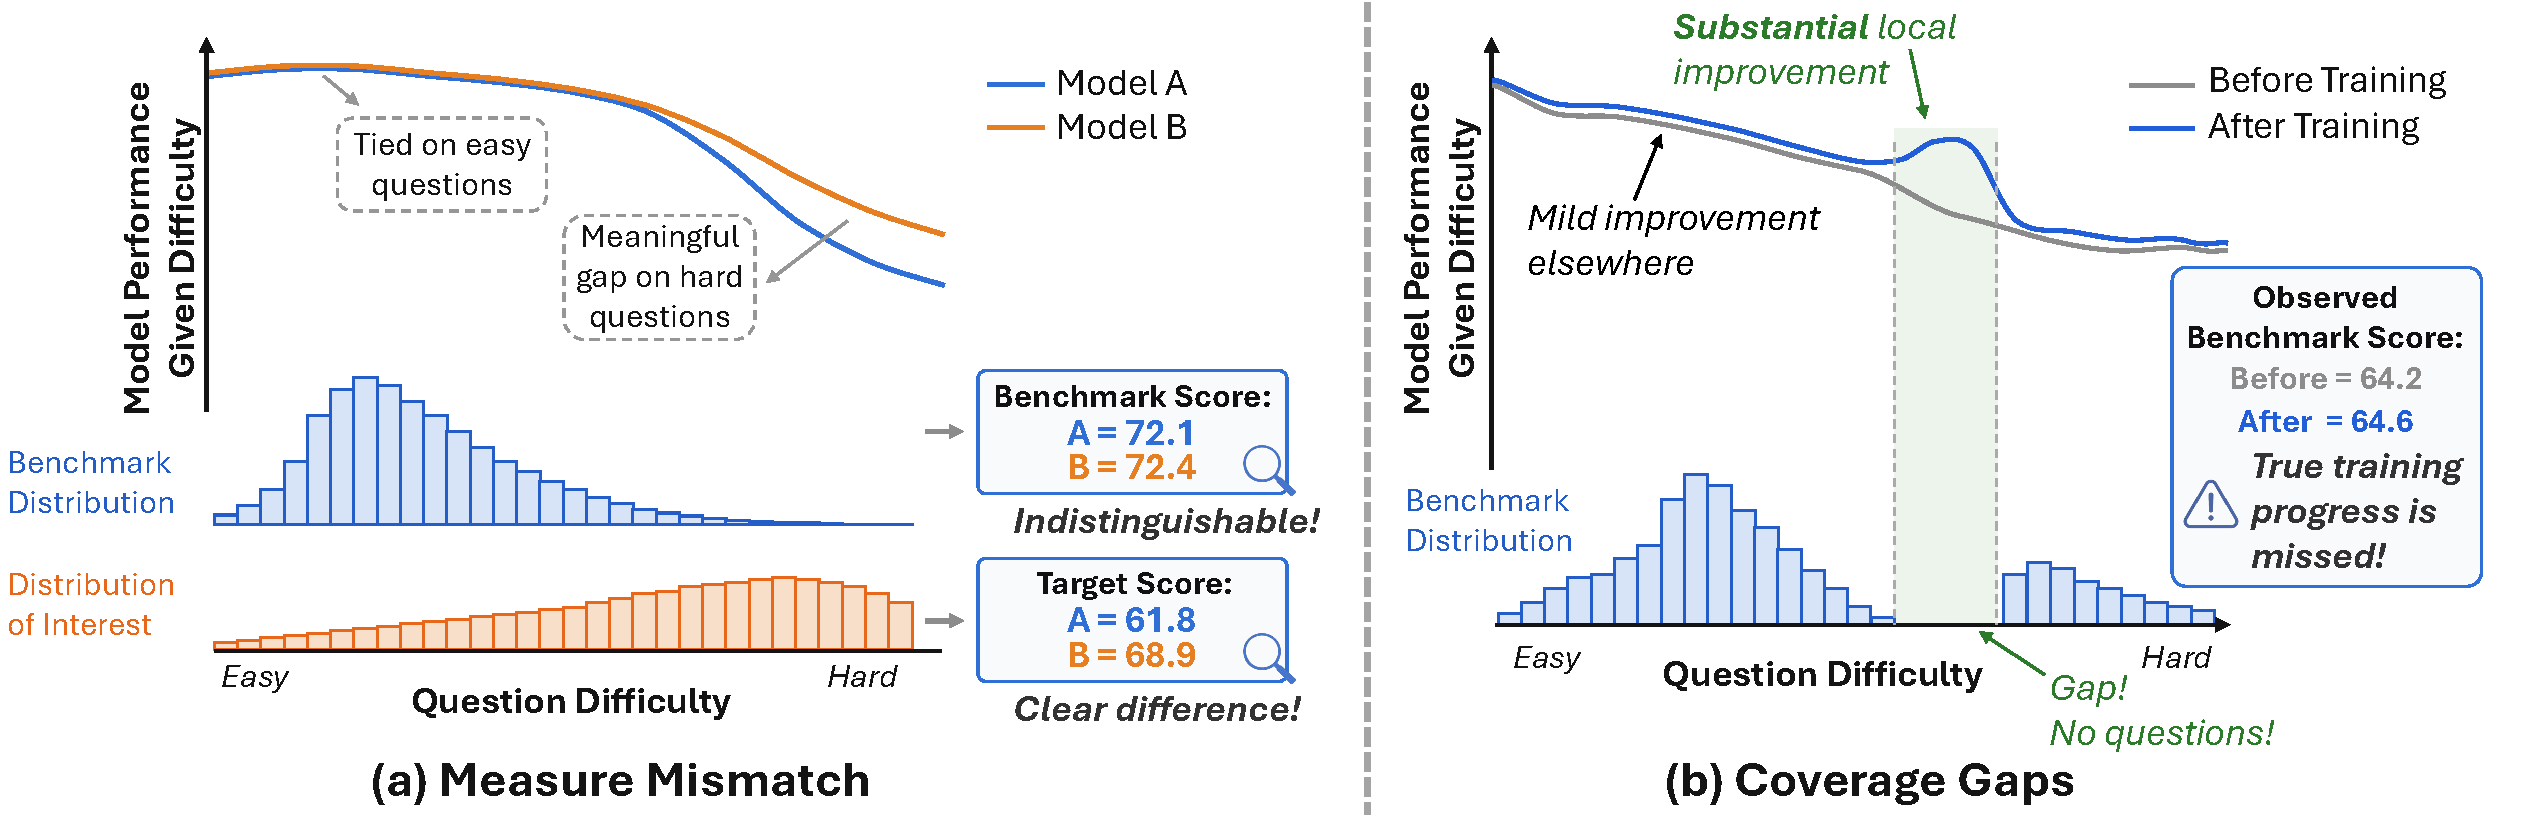
\includegraphics{Fig/teaser.pdf}}
      \vspace{-4mm}
    \caption{\textbf{两种基准失效情形。} 两幅图中的曲线均表示真实模型的\textit{条件}性能，即\textit{作为题目难度的函数}。
    (a) \textbf{测度失配。}
    基准强调简单题，而模型在简单题上表现相近；我们关心的难度分布则把更多权重放在更难的题目上，模型在这些题目上差异很大。
    由于基准与目标分布对难度轴的加权不同，它们对同一对模型给出不同结论。
    % As a result, the benchmark suggests a near tie, whereas the target evaluation shows a clear separation.
    (b) \textbf{覆盖缺口。} 模型实际上在某个局部难度区域上有\textit{显著}提升。由于基准在该区域没有题目，这一提升没有反映在观测到的基准分数中，导致有意义的训练进展被遗漏。}
    \label{fig:teaser}
  \vspace{-6mm}
\end{figure}

\section{形式化与理论}

\paragraph{难度空间与模型性能函数。}
我们用连续变量 $z\in[0,1]$ 表示基准题目（例如一道题）的难度，较大的值对应较难的题目。对模型 $\theta$，令 $s_\theta(z)\in[0,1]$ 表示其在难度为 $z$ 的题目上的条件期望性能，例如 pass@1。
  \vspace{-2mm}
\paragraph{基准分布与分数。}
设基准 $B=\{x_i\}_{i=1}^n$ 由 $n$ 道题组成，并令
$z_i\in[0,1]$ 表示题目 $x_i$ 的难度。基准分数为 $S_B(\theta):=\frac{1}{n}\sum_{i=1}^n s_\theta(z_i)$。这一平均隐式地在难度轴上诱导出一个经验测度，
\[
\nu_B=\frac{1}{n}\sum_{i=1}^n \delta_{z_i},
\]
其中 $\delta_z$ 表示位于难度 $z$ 处的点质量。在这一表示下，基准分数恰好是关于基准所诱导难度测度的积分，$S_B(\theta)=\int s_\theta(z)\,d\nu_B(z)$。

\paragraph{两个模型之间的性能差。}
对两个模型 $\theta$ 与 $\theta'$，定义\emph{难度条件下的性能差}为 $\Delta(z):=s_{\theta'}(z)-s_\theta(z)$，为记号简便，省略 $\Delta$ 对 $(\theta',\theta)$ 的依赖。\textit{在基准 $B$ 上观测到的}性能差为
\[
D_B(\theta',\theta)
:= S_B(\theta')-S_B(\theta)
= \frac{1}{n}\sum_{i=1}^n \Delta(z_i)
= \int \Delta(z)\,d\nu_B(z).
\]

\subsection{测度失配}
\paragraph{基准诱导的耦合。}
量 $D_B(\theta',\theta)$ 隐式地耦合了两个不同对象：\textit{依赖模型的函数} $\Delta(z)$ 与\textit{依赖基准的测度} $\nu_B$。因此，排行榜比较并非仅由模型之间难度条件下的性能差决定；它还取决于基准如何在难度轴上分配质量。若这一分配不同于我们关心的难度分布，基准就会在失配的测度下聚合同一模型差异。这种失配可能扭曲观测到的模型差距，在严重情形下还会改变所诱导的排序。

\paragraph{目标分布。}
形式上，我们引入目标分布
$
\mu \in \mathcal{P}([0,1]),
$
它表示难度空间上预期的评测分布。该目标分布可以编码期望的应用组合。在 $\mu$ 下，模型 $\theta$ 的目标分数以及 $\theta'$ 与 $\theta$ 之间的目标性能差定义为
\[
S_\mu(\theta)
:=
\int s_\theta(z)\, d\mu(z),
\qquad
D_\mu(\theta',\theta)
:=
S_\mu(\theta') - S_\mu(\theta)
=
\int \Delta(z)\, d\mu(z).
\]

$D_B(\theta',\theta)$ 与 $D_\mu(\theta',\theta)$ 之间的差异来自基准测度 $\nu_B$ 与目标分布 $\mu$ 的失配。这一观点使我们可以把排行榜比较中的扭曲作为分布失配问题来研究。

\paragraph{分布失配的度量。}
我们用 1-Wasserstein 距离衡量基准的难度分布与目标难度分布的匹配程度。具体地，对经验难度测度为 $\nu_B$ 的基准 \(B\) 以及 \([0,1]\) 上的目标分布 \(\mu\)，我们将其\emph{难度分布失配（Difficulty Distribution Mismatch, DDM）}定义为
\[
\mathrm{DDM}(B;\mu) := W_1(\nu_B,\mu)
=
\inf_{\pi \in \Pi(\nu_B,\mu)}
\int_{[0,1]^2} |u-v|\, d\pi(u,v),
\]
其中 $\Pi(\nu_B,\mu)$ 表示 $\nu_B$ 与 $\mu$ 的所有耦合构成的集合。直观上，$W_1(\nu_B,\mu)$ 衡量要把基准难度分布变换成目标分布，需要搬运多少概率质量、以及搬运多远。下面的定理表明，这种失配直接控制基于基准与基于目标的性能差之间的扭曲。



\begin{theorem}[分布失配控制分数扭曲与排名稳定性]
\label{thm:w1_rank_stability}
设性能差函数 $\Delta$ 是 $L$-Lipschitz 的。则
\[
\bigl|D_B(\theta',\theta) - D_\mu(\theta',\theta)\bigr|
\le
L\, W_1(\nu_B,\mu).
\]
因此，若 $|D_\mu(\theta',\theta)| > L\, W_1(\nu_B,\mu)$，则
\[
\operatorname{sign}\bigl(D_B(\theta',\theta)\bigr)
=
\operatorname{sign}\bigl(D_\mu(\theta',\theta)\bigr),
\]
从而基准所诱导的排序与目标排序一致，即不会发生排名翻转。
\end{theorem}



定理~\ref{thm:w1_rank_stability} 表明，$W_1(\nu_B,\mu)$ 界定了基准所诱导的分数差与目标分数差之间可以相差多少。较小的 $W_1(\nu_B,\mu)$ 意味着基准是目标评测的忠实近似，而较大的 $W_1(\nu_B,\mu)$ 表明基准可能过度强调某些难度区域、同时低估另一些区域，从而可能扭曲模型比较，甚至改变其诱导排名。附录~\ref{sec:app_proof_mismatch} 给出完整证明，并将该结果推广到有限样本设定。



\paragraph{无先验信息时有原则的目标分布。}
当已有先验信息时，自然应选择 $\mu$ 以反映难度空间上预期的评测目标。然而在许多设定中，此类先验知识不可得。此时，选择非均匀目标会在没有证据的情况下隐含地偏袒某些难度区域。为刻画一个有原则的默认选择，我们考虑一种不可知设定：性能差沿难度轴出现的位置完全未知。我们考虑函数类
\[
\mathcal{F}_{\rho}
:=
\left\{
\Delta:[0,1]\to[-1,1]\ \text{可测} :
\int_0^1 \Delta(z)\,dz = \rho
\right\},
\qquad \rho\in(-1,1).
\]
该类编码一个不确定性集合：带符号的性能差在难度轴上具有固定的平均水平 $\rho$，但其位置除此之外不受限制。

对任意候选目标分布 $\mu \in \mathcal P([0,1])$，定义其最坏情形保留差为
\[
V_{\rho}(\mu)
:=
\inf_{\Delta \in \mathcal{F}_{\rho}}
\int \Delta(z)\, d\mu(z).
\]
下面的定理表明，当对性能差沿难度轴出现的位置完全不确定时，均匀分布是\textit{唯一}的极大极小（maximin）目标，并且是唯一使最坏情形保留差仍等于平均差 $\rho$ 的选择。

\begin{theorem}[均匀目标是唯一的极大极小选择]
\label{thm:uniform_maximin}
对 $\rho \in (-1,1)$，我们有
\[
\sup_{\mu \in \mathcal P([0,1])} V_{\rho}(\mu) = \rho,
\]
且唯一的最大化子是均匀分布 $\lambda=\mathrm{Unif}[0,1]$。
\end{theorem}
定理~\ref{thm:uniform_maximin} 并不声称均匀分布在一切情形下都最优。它只是在难度空间上没有先验信息时，为把均匀分布作为有原则的默认目标提供依据。此时，采用均匀目标避免了对难度区域引入额外偏好，并为基准评测提供一条中性准则：评测并不先验地偏袒任何难度区域。完整证明见附录~\ref{sec:app_proof_mismatch}。


\subsection{覆盖缺口}

\paragraph{离散的基准测度可能无法监测局部训练改进。}
基准不仅常用于最终的模型比较，也用于监测训练进展~\citep{he2025skywork,yu2025dapo,luo2025deepscaler}。然而，训练改进往往是局部的而非均匀的：模型可能在某一特定难度范围内大幅提升，而在其他地方仅有适度改进。

回想基准分数是关于基准经验测度 $\nu_B$ 的积分。由于 $\nu_B$ 是\textit{离散}测度，仅支撑在有限个基准难度点上，它对每一个不含基准题目的区间都赋予零质量。因此，即使模型在一段非平凡的连续难度区域上有显著改进，只要该区域不含基准题目，基准分数也可能反映不出这一改进。在这个意义上，当局部分辨率不足时，基准作为进展监测器会失效。

% This raises a natural question: when a model improves over a contiguous difficulty region, under what conditions can a benchmark detect that improvement? To study this, we first characterize the local resolution of a benchmark through its \emph{maximum gap}.

% This motivates the following question: when a model improves on a contiguous region of the difficulty axis, under what conditions is that improvement statistically detectable from benchmark evaluations? To formalize this question, we first characterize the local resolution of a benchmark through its \emph{maximum gap}, which measures the largest uncovered region of the difficulty axis. We then study statistical detectability through a hypothesis testing framework, where the null hypothesis corresponds to no performance change and the alternative corresponds to a localized improvement of a given width and magnitude.

\paragraph{最大间隔。}
我们首先用\emph{最大间隔}刻画基准的局部分辨率。令 $0 \le z_{(1)} \le \cdots \le z_{(n)} \le 1$ 为有序的基准难度点，并定义 $z_{(0)}:=0$ 与 $z_{(n+1)}:=1$。基准 $B$ 的\emph{最大间隔}为
\begin{equation}
G(B):=\max_{0\le j\le n}\bigl(z_{(j+1)}-z_{(j)}\bigr)
\label{eq:max_gap}
\end{equation}
即难度轴上不含任何基准点的最大区间的长度。

\paragraph{假设检验表述。}
为形式化基准能否可靠检测局部训练改进，我们将该问题表述为假设检验。在原假设下没有改进。在备择假设下，改进后的性能在某个宽度为 $w$ 的连续难度区间上，至少比改进前高出 $a$。下面的定理表明，基准最大间隔 $G(B)$ 正是精确的渐近极小极大检测边界。

\begin{theorem}[最大间隔作为精确的渐近极小极大检测边界]
\label{thm:max-gap-detection-boundary}
固定检验水平 $\alpha\in(0,1)$ 与 $a\in(0,1]$。令 $s^-,s^+:[0,1]\to[0,1]$ 分别表示改进前与改进后的性能曲线。对基准 $B$，令 $\Pi_\alpha^*(B;w,a,k)$ 表示：基于每道基准题 $k$ 次重复样本、用于检验
\[
H_0:\ s^-=s^+
\qquad\text{对}\qquad
H_1:\ \exists\ \text{区间 } I\subset[0,1],\ |I|=w,\  s^+(z)-s^-(z)\ge a\ \ \forall z\in I.
\]
的水平 $\alpha$ 检验的极小极大最坏情形功效。
\begin{enumerate}
    \item 若 $w \le G(B)$，则对每个 $k\in\mathbb N$，有 $\Pi_\alpha^*(B;w,a,k)=\alpha$。
    \item 若 $w > G(B)$，则 $\lim_{k\to\infty}\Pi_\alpha^*(B;w,a,k)=1$。
\end{enumerate}
因此，$G(B)$ 精确刻画了基准 $B$ 的渐近极小极大检测边界。
\end{theorem}




定理~\ref{thm:max-gap-detection-boundary} 表明，基准的离散几何诱导出一个尖锐的可检测性相变。若局部改进的宽度不超过相邻难度点的最大间隔，则无论重复评测多少次，任何水平 $\alpha$ 的检验都无法取得非平凡的最坏情形功效。换言之，在最坏情形下，这样的改进对基准可以完全不可见。一旦改进宽度超过最大间隔，重复评测最终可以使该信号可检测。在这个意义上，$G(B)$ 刻画了基准 $B$ 固有的局部分辨率极限。
完整证明见附录~\ref{sec:app_proof_missed}。
% The full proof along with two additional geometric interpretations of the maximum gap are given in App.~\ref{sec:app_proof_missed}: a deterministic lower bound on benchmark response to a localized improvement, and a random-location formula for complete-miss probability.

\section{当前基准的实证诊断}

\begin{figure}[t]
    \centering
    \resizebox{\textwidth}{!}{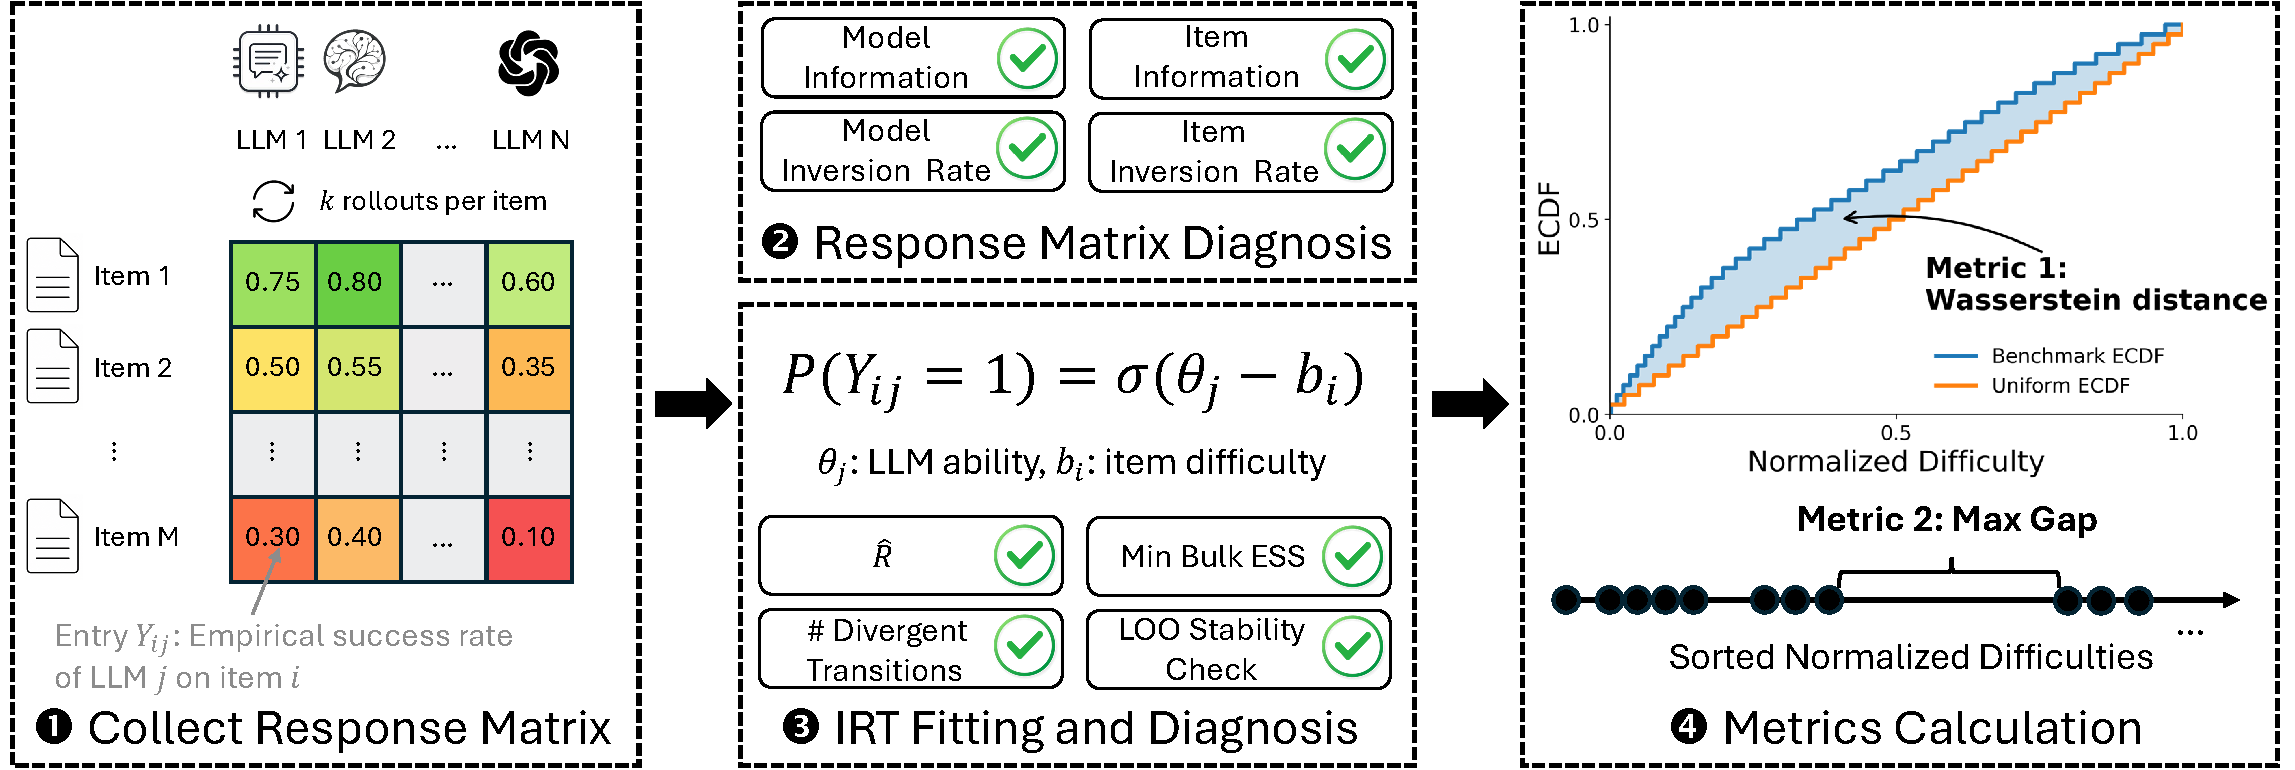
\includegraphics{Fig/pipeline.pdf}}
      \vspace{-4mm}
    \caption{\textbf{基准难度估计与指标计算流程概览。} 我们收集多个 LLM 在基准题目上的经验成功率，诊断响应矩阵，拟合 1PL IRT 模型以估计题目难度，进行拟合后的 IRT 诊断，并在归一化难度分布上计算两个指标。
    % Wasserstein-based distribution mismatch and the maximum adjacent difficulty gap.
    }
    \label{fig:pipeline}
  \vspace{-4mm}
\end{figure}
我们用前文提出的两个指标，分析一组来自不同领域、被广泛使用的基准。图~\ref{fig:pipeline} 给出难度估计与指标计算流程的概览。具体而言，我们考虑涵盖数学、编程、智能体任务、逻辑、科学、指令遵循与医学的 \textbf{25} 个常用基准。这些基准的详细信息见附录~\ref{sec:app_benchmark_details}。

\subsection{难度估计与指标计算}

\paragraph{方法：项目反应理论。}
为估计基准题目难度，人们可能会直接使用每道题在各模型上的平均失败率~\citep{yu2025dapo,sun2026improving,wen2025light}。然而，题目难度本质上相对于模型能力：它不仅应取决于有多少模型答错该题，还应取决于答错或答对该题的模型有多强。
% Average failure rate ignores the abilities of the models behind these successes and failures. 
因此我们使用项目反应理论（IRT）。它是一个成熟的心理测量框架~\citep{lord1952theory, rasch1993probabilistic}，已被广泛用于 LLM 基准分析中的难度估计~\citep{ding2024easy2hard, rodriguez2021evaluation, hofmann2025fluid, kipnis2024metabench, polo2024tinybenchmarks, zhou2026lost}。IRT 将模型解出一道题的概率建模为模型能力与题目难度的函数。在常用的单参数 logistic 模型（1PL）中，每个模型 $j$ 被赋予能力参数 $\theta_j$，每道题 $i$ 被赋予难度参数 $b_i$。模型 $j$ 正确解出题目 $i$ 的概率建模为
\[
\Pr(Y_{ij}=1)=\sigma(\theta_j-b_i),
\]
其中 $\sigma(\cdot)$ 为 logistic 函数。直观上，$b_i$ 越大的题目需要越高的模型能力才能被正确解出，因此估计得到的 $b_i$ 提供了题目难度的自然度量。对选择题基准，上述模型可以自然地用猜测参数加以扩展。

实践中，难度估计首先收集多个模型在基准题目上的表现，形成响应矩阵 $Y \in \mathbb{R}^{n \times m}$，其中 $Y_{ij}$ 表示模型 $j$ 在题目 $i$ 上的经验成功率。随后通过拟合 IRT 模型所诱导的似然，估计潜在能力 $\{\theta_j\}_{j=1}^m$ 与题目难度 $\{b_i\}_{i=1}^n$。
% This is typically done via maximum likelihood or Bayesian estimation methods (e.g., Markov chain Monte Carlo (MCMC) or variational inference). 
为确保难度估计可靠，我们采取若干实际措施，包括\textbf{审慎的模型选择}与\textbf{严格的 IRT 拟合诊断}。

\paragraph{模型选择。}
准确的难度估计需要能力水平多样的模型。为确保充分的能力覆盖，我们有意选择跨越宽能力范围的模型。对非智能体基准，我们依据 Text Arena 的公开排行榜\footnote{\url{https://arena.ai/leaderboard}} 选择 $12$ 个 LLM，参数规模从 $1.7$B 到 $397$B。模型首先按跨多个领域汇总的总体能力排序，再沿该排名划分为若干近似等长的区间。我们通过从每个区间选取一个模型进行分层抽样，并额外纳入排名顶部与底部的若干模型，以更好地覆盖能力谱的两端。每个被选模型在每道基准题上最多进行 $32$ 次 rollout，使用模型推荐的 temperature 与 top-$p$。对智能体基准，任务通常需要较强的专有模型。因此我们依赖 HAL~\cite{hal} 的评测结果，它报告了 $15$--$66$ 个最先进闭源 LLM 在智能体任务基准上的表现。模型的详细信息见附录~\ref{sec:app_model_details}。

\paragraph{IRT 拟合与诊断。}
我们通过 MCMC 进行贝叶斯推断来估计 IRT 参数。为确保难度估计可靠，我们在 IRT 拟合\textit{之前}与\textit{之后}都进行一系列诊断。拟合前，我们用 $4$ 个指标检查响应矩阵的信息量与结构一致性。拟合后，我们用 $3$ 个标准贝叶斯诊断评估收敛性与采样质量，包括 Gelman--Rubin 统计量（$\hat{R}$）、有效样本量（ESS）以及发散转移的次数。所有基准都通过了全部 $7$ 项诊断检查。
对非智能体基准，我们进一步进行留一法（leave-one-out, LOO）稳健性分析。结果表明，我们选择的 $12$ 个模型足以得到稳定的难度估计。为支持后续工作，我们还公开发布了这 $25$ 个基准经过仔细整理的难度估计\footnote{\url{https://github.com/ASTRAL-Group/benchmark-difficulty-measure/tree/main/data/benchmarks}}。详细定义与诊断结果见附录~\ref{sec:app_irt}。我们还在附录~\ref{app:irt_model_comparison} 中提供了与 2PL 及多维 IRT 模型的额外模型比较分析。

% For non-agentic benchmarks, we further conduct a leave-one-out (LOO) robustness analysis. Specifically, we refit IRT after removing each model in turn, and measure the consistency between the resulting item difficulties and the original estimates. Averaged over the $12$ LOO refits within each benchmark, both the Spearman and Pearson correlations are at least $0.97$ for every benchmark, indicating that our choice of $12$ models is sufficient for stable difficulty estimation. To support future work, we will open-source the carefully curated difficulty estimates for the $25$ benchmarks. Detailed definitions and results are provided in App.~\ref{sec:app_irt}.

% For non-agentic benchmarks, we also perform a leave-one-out robustness analysis over the selected model set; averaged over leave-one-out refits and benchmarks, both the Pearson and Spearman correlations with the original difficulty estimates exceed $0.97$, indicating highly stable difficulty estimation (App.~\ref{sec:app_irt}).

\paragraph{所提出指标的计算。}
对每个基准，在估计题目难度后，我们首先将其归一化到 $[0,1]$，并计算其经验累积分布函数（ECDF）。由于一般情况下难度空间上没有额外先验信息，我们通过计算基准经验测度与 $[0,1]$ 上同规模经验\textit{均匀参照}之间的 1-Wasserstein 距离来量化分布失配。在一维情形下，这等价于它们 ECDF 之间的 $L_1$ 距离。我们按式~\eqref{eq:max_gap} 计算最大间隔，并同时报告五个最大相邻间隔之和作为参照指标。两个指标的后验不确定性分析见附录~\ref{app:metric_uncertainty}。

\subsection{结果与分析}

\paragraph{若干基准相对中性均匀目标存在较大偏离。} 表~\ref{tab:main_result} 显示，25 个基准中有 10 个满足 $\mathrm{DDM}\ge 0.10$，表明其经验难度分布平均至少需要搬运整个难度范围的 10\%，才能与同规模均匀参照相匹配。因此这些基准编码了很强的隐含难度加权：其汇总分数对过度代表的难度区域更敏感，对代表不足的区域更不敏感。当非均匀性与预期评测目标一致时，它本身并非问题。然而，若未指定这样的目标，高 DDM 的排行榜结果不应被解读为难度中性的比较。相反，它们反映的是在该基准经验难度加权下的比较，因此使用者应检查这一加权是否与其使用场景相关的难度分布相符。附录~\ref{sec:app_benchmark_cal} 给出一个简单的基准校准算法，用于使基准分布更接近选定的目标。

\paragraph{许多基准存在较大的局部覆盖缺口。}
表~\ref{tab:main_result} 显示，25 个基准中有 8 个满足 $\mathrm{Max\ Gap}\ge 0.10$。因此，一次训练可能在未被覆盖的难度区域取得有意义的局部进展，而汇总基准分数几乎不变。这会导致有用的训练进展被低估，有希望的运行被过早放弃，计算资源被错误分配。此外，问题并不限于单一的最大间隔。我们发现 25 个基准中有 9 个满足 $\mathrm{Top\text{-}5\ Sum}\ge 0.30$。例如，图~\ref{fig:main_result} 显示 AIME24 与 AIME25 的前 5 大间隔之和接近 $0.5$，尽管它们被广泛用于监测 RLVR 训练~\cite{luo2025deepscaler,liu2025prorl,guo2025deepseek,yue2025vapo}，难度轴上仍有大段局部未分辨。

我们指出，尽管 $\mathrm{Max\ Gap}$ 本质上依赖于基准规模，这反映的是真实的覆盖限制，而不仅仅是需要消除的干扰效应：即使小基准预期会有较大间隔，它仍然是一段未被覆盖的难度区间，并且由定理~\ref{thm:max-gap-detection-boundary}，落在该区间内的局部改进在最坏情形下可能不可检测。重要的是，我们发现覆盖缺口并非仅仅是小基准的产物：拥有数百道题的基准，例如 HumanEval 与 BBH-5 objects，也表现出可观的间隔指标。这促使我们将缺口填补作为提高基准局部分辨率的一种实用且必要的途径。

\begin{figure*}[t]
    \centering
    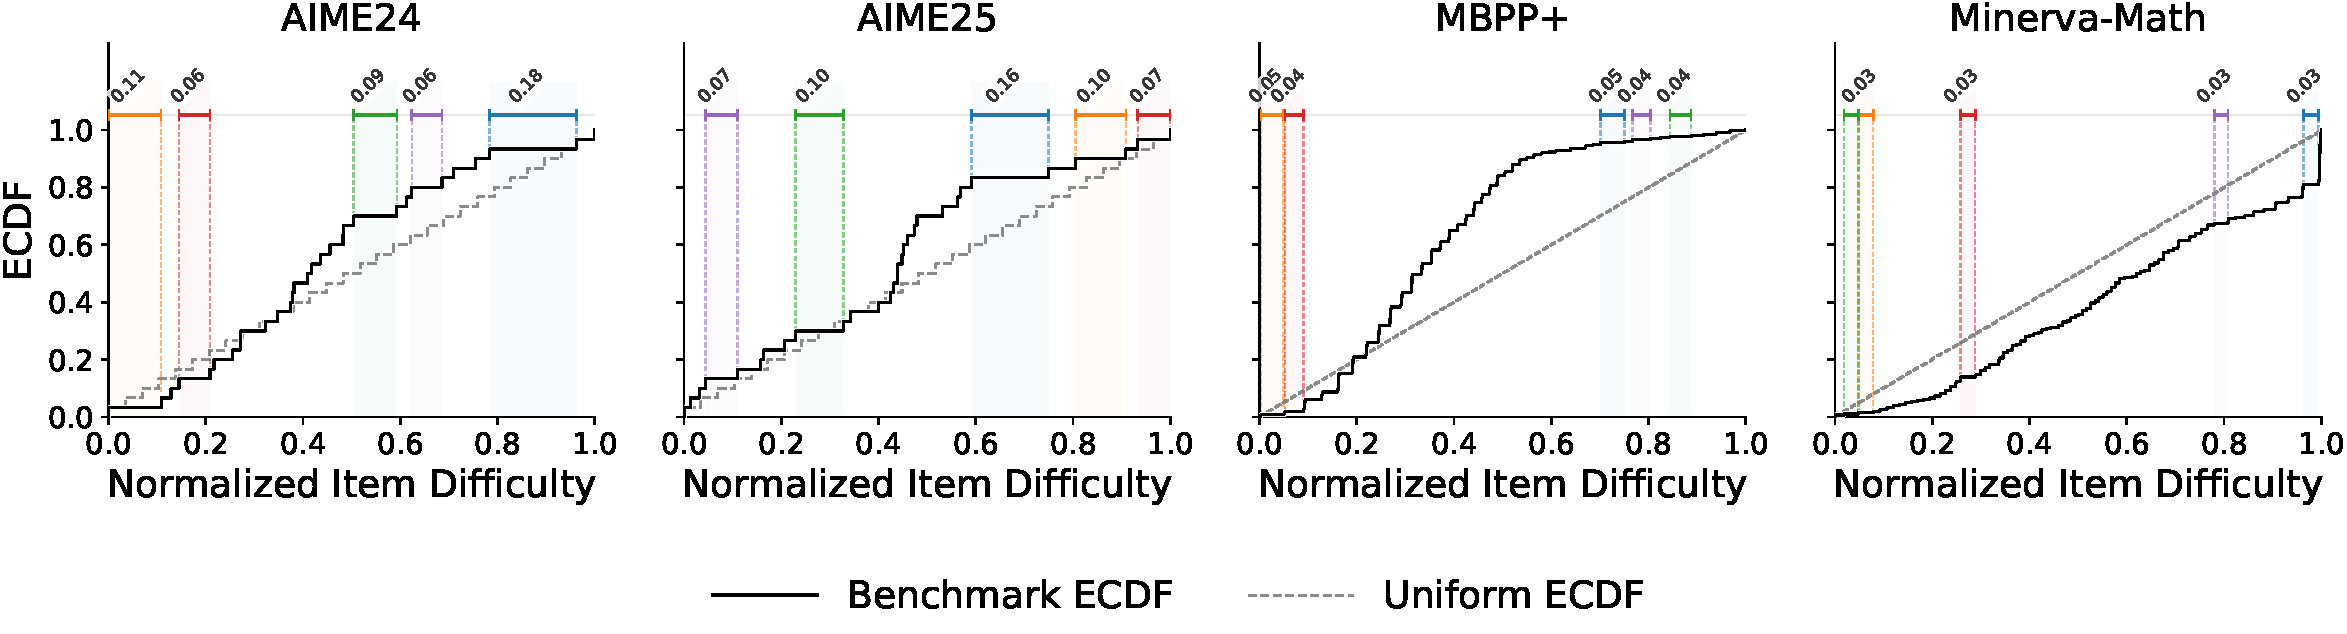
\includegraphics[width=\textwidth]{Fig/main_result.pdf}
  \vspace{-4mm}

    \caption{\textbf{基准难度分布。}
    每个面板展示一个基准归一化题目难度的 ECDF，以及中性均匀参照。彩色阴影区间标出五个最大的相邻难度间隔，标签为相应的间隔大小。更多基准示例见图~\ref{fig:appendix_result}。}
    \label{fig:main_result}
    \vspace{-4mm}
\end{figure*}

\begin{table*}[t]
\centering
\caption{\textbf{各基准上所提出指标的汇总。}
$\mathrm{DDM}$ 表示基准经验难度分布与 $[0,1]$ 上同规模经验均匀分布之间的 1-Wasserstein 距离。$\mathrm{Max\ Gap}$ 是归一化难度相邻点之间的最大间隔，$\mathrm{Top\text{-}5\ Sum}$ 是五个最大此类间隔之和。\# 表示基准题目数。三个指标均越低越好。高亮条目标出各指标相对较大的值：$\mathrm{DDM}\ge 0.10$，$\mathrm{Max\ Gap}$ $\ge 0.10$，或 $\mathrm{Top\text{-}5\ Sum}$ $\ge 0.30$。}
\label{tab:main_result}
\small
\begin{minipage}[t]{0.49\linewidth}
\vspace{0pt}
\centering
\resizebox{\linewidth}{!}{
\begin{tabular}{l r r r r}
\toprule
\textbf{基准} &
\textbf{$\mathrm{DDM}$} & \textbf{$\mathrm{Max\ Gap}$} & \textbf{$\mathrm{Top\text{-}5\ Sum}$} & \textbf{\#} \\
\midrule
MATH-500 & \highddm{0.164} & 0.058 & 0.175 & 500 \\
Minerva-Math & \highddm{0.122} & 0.031 & 0.149 & 272 \\
OlympiadBench & 0.064 & 0.048 & 0.142 & 675 \\
Gaokao2023en & 0.088 & 0.055 & 0.183 & 385 \\
AMC23 & 0.089 & \highddm{0.217} & \highddm{0.539} & 40 \\
AIME24 & 0.077 & \highddm{0.179} & \highddm{0.502} & 30 \\
AIME25 & 0.079 & \highddm{0.158} & \highddm{0.492} & 30 \\
AIME26 & 0.085 & \highddm{0.119} & \highddm{0.507} & 30 \\
MMLU-Pro-Biology & \highddm{0.125} & 0.045 & 0.151 & 717 \\
MMLU-Pro-Chemistry & \highddm{0.114} & 0.072 & 0.192 & 1132 \\
MMLU-Pro-Physics & \highddm{0.121} & 0.035 & 0.157 & 1299 \\
GPQA-Diamond & 0.080 & 0.066 & 0.263 & 198 \\
ScienceQA & \highddm{0.178} & 0.045 & 0.175 & 4241 \\
\bottomrule
\end{tabular}
}
\end{minipage}
\hfill
\begin{minipage}[t]{0.49\linewidth}
\vspace{0pt}
\centering
\resizebox{\linewidth}{!}{
\begin{tabular}{l r r r r}
\toprule
\textbf{基准} &
\textbf{$\mathrm{DDM}$} & \textbf{$\mathrm{Max\ Gap}$} & \textbf{$\mathrm{Top\text{-}5\ Sum}$} & \textbf{\#} \\
\midrule
HumanEval & \highddm{0.148} & \highddm{0.165} & \highddm{0.423} & 164 \\
MBPP+ & \highddm{0.163} & 0.049 & 0.214 & 378 \\
GAIA & 0.084 & 0.051 & 0.218 & 165 \\
CORE-Bench Hard & 0.036 & \highddm{0.113} & \highddm{0.363} & 45 \\
SWE-bench-Mini & 0.053 & \highddm{0.149} & \highddm{0.469} & 50 \\
USACO & 0.080 & 0.082 & \highddm{0.354} & 307 \\
IFEval & \highddm{0.159} & 0.046 & 0.189 & 541 \\
BBH-3 objects & 0.090 & 0.075 & 0.294 & 250 \\
BBH-5 objects & 0.099 & \highddm{0.128} & \highddm{0.332} & 250 \\
BBH-7 objects & 0.077 & 0.059 & 0.279 & 250 \\
ZebraLogic & 0.080 & 0.027 & 0.127 & 1000 \\
MedQA & \highddm{0.157} & 0.042 & 0.178 & 1273 \\
\bottomrule
\end{tabular}
}
\end{minipage}
    \vspace{-4mm}

\end{table*}

\section{\textsc{BenchFill}：面向难度的缺口填补}

\begin{figure*}[t]
    \centering
    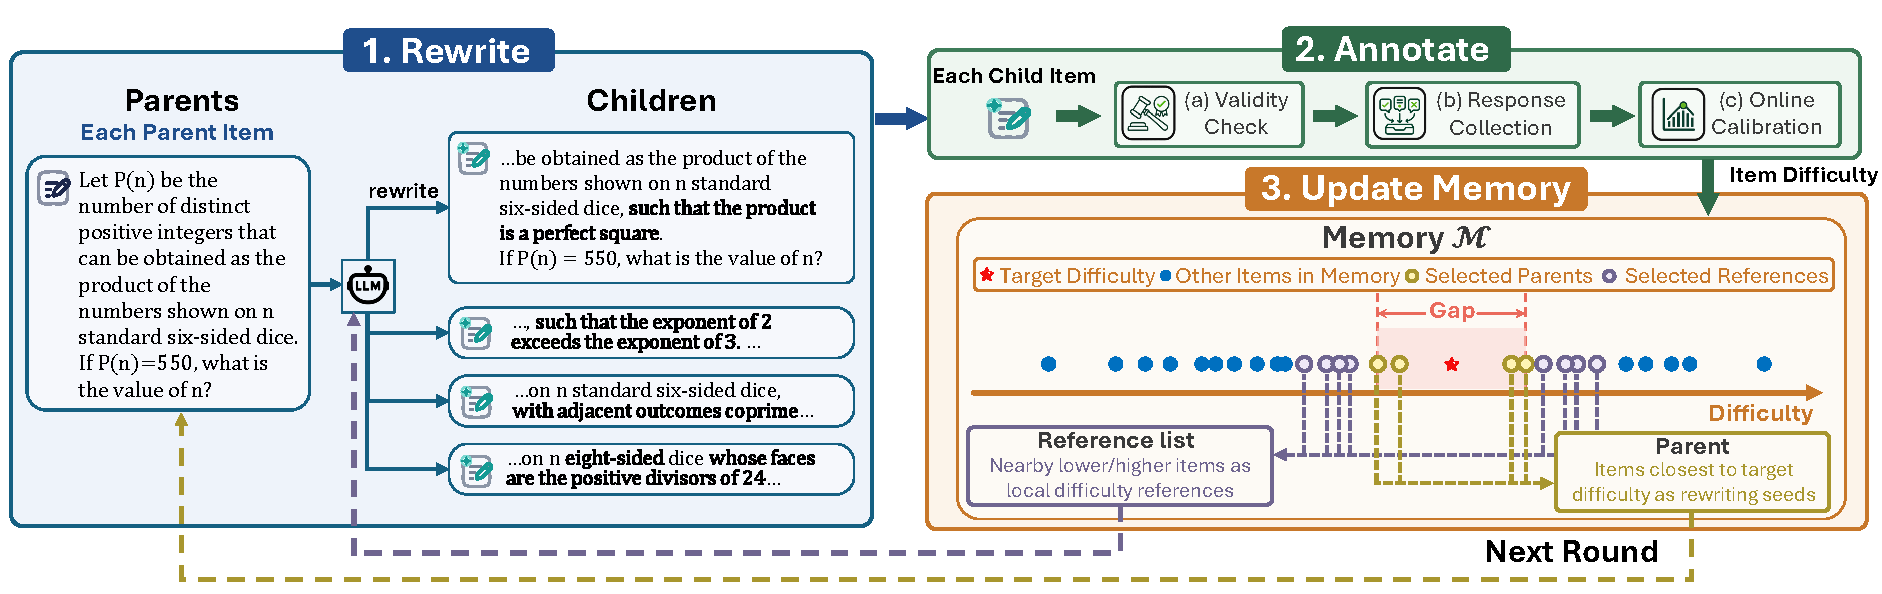
\includegraphics[width=\textwidth]{Fig/search.pdf}
      \vspace{-4mm}
    \caption{\textbf{\textsc{BenchFill} 概览。}
    \textsc{BenchFill} 迭代地将父题改写为子变体，标注其难度，并更新记忆以指导下一轮缺口填补。}
    \label{fig:benchfill_overview}
  \vspace{-4mm}
\end{figure*}

\subsection{问题设定与方法}

% As discussed above, large gaps in the difficulty distribution limit a benchmark's local resolution.
% By Theorem~\ref{thm:max-gap-detection-boundary}, reducing these gaps improves the benchmark's ability to capture localized model improvements. 
% As discussed above, reducing large gaps in the difficulty distribution improves a benchmark's local resolution and its ability to capture localized model improvements. In this section, we introduce \textsc{BenchFill}, a propose-and-annotate evolutionary search algorithm~\citep{sharma5openevolve,liu2026evox} for difficulty-targeted item rewriting. Rather than generating items from scratch, \textsc{BenchFill} iteratively rewrites existing benchmark items, estimates the difficulties of the rewritten variants, and stores the resulting item--difficulty pairs in a memory bank. This memory guides subsequent rewrites toward under-covered regions of the difficulty axis. The complete pseudocode is provided in Alg.~\ref{alg:gap_filling}.
% The algorithm proceeds iteratively. At each round, it proposes a set of candidate benchmark items, estimates their difficulties, and stores the resulting item--difficulty pairs in a memory bank for subsequent proposals. By conditioning new generations on previously observed item--difficulty pairs, the search gradually moves toward the target difficulty and produces items that effectively fill the identified gaps. 
% The complete pseudocode is provided in Alg.~\ref{alg:gap_filling}.

\paragraph{问题设定。}
令 $B=\{x_i\}_{i=1}^n$ 为当前基准，其中每道题 $x_i$ 具有估计难度 $z_i$。我们将难度排序，并考虑两道基准题之间的相邻间隔 $[z_L,z_R]$。缩小此类间隔可以提高基准的局部分辨率及其捕捉局部模型改进的能力。因此，我们的目标是得到一道有效的新题 $x_{\mathrm{new}}$，其难度尽可能接近目标难度 $z^\star=(z_L+z_R)/2$，即单次插入下最能缩小该间隔的中点。新题被加入基准，而不是替换任何已有题目。默认情况下，我们对该基准的\textit{最大}间隔应用这一过程。

一种直接做法是请人类专家按目标难度设计新题，但这一过程可能代价高昂~\cite{rein2024,phan2025humanity}。受近期关于 LLM 辅助基准扩充的工作启发~\cite{cheng2026vera,li2025ride,ying2024automating,xia2024top}，我们改为使用 LLM 将已有基准题\textit{改写}为针对目标难度的新变体。这种基于改写的方法可扩展，以已有题目作为局部参照来控制难度调整，并有助于保持原始基准的格式与风格。为确保题目质量，最终入选的题目还会由人类专家进一步验证。接下来我们介绍 \textsc{BenchFill}，一种用于自动、面向目标难度的题目改写的“改写并标注”进化搜索算法~\citep{sharma5openevolve,liu2026evox}。算法~\ref{alg:gap_filling} 给出伪代码，图~\ref{fig:benchfill_overview} 说明该过程。

\paragraph{\textsc{BenchFill}。}
给定目标难度 $z^\star$，算法维护一个由已标注题目--难度对组成的记忆 $\mathcal{M}$。记忆用难度最接近所选间隔的已有基准题初始化，并在搜索过程中更新。每一轮执行一步父--子改写。\emph{父题}是从 $\mathcal{M}$ 中选出、作为改写主要参照的已有题目或先前改写得到的题目，而\emph{子题}是由父题派生的新提议变体。


在第 $t$ 轮，我们从 $\mathcal{M}$ 中检索一小批标注难度最接近目标难度 $z^\star$ 的父题。对每个父题，改写 LLM 以该父题、目标难度以及附近题目--难度对的参照列表为条件。参照列表提供 $z^\star$ 附近的局部样例，通常包括略低于和略高于目标难度的题目，例如当 $z^\star=0.55$ 时，难度为 $0.48,0.50,0.60$ 与 $0.62$ 的题目。随后改写器将每个父题改写为一批子题，同时保持基准的格式与风格。


改写之后，每个子题被送入下文详述的难度标注模块，该模块返回估计难度 $\hat{z}$。我们只保留有效\footnote{我们使用 GPT-5.4 作为有效性评判器，核验每道改写题目所附答案是否正确。}的子题，并将其标注后的题目--难度对 $(x,\hat{z})$ 加回 $\mathcal{M}$。这一更新使搜索具有自适应性：每当某个改写子题比先前题目更接近 $z^\star$，它在后续轮次中就更可能被检索为父题或进入参照列表。因此，随着搜索推进，改写器以越来越与目标相关的样例为条件，而不是独立地改写每一批。经过 $T$ 轮后，我们选择使 $|\hat{z}-z^\star|$ 最小的有效子题作为提议的缺口填补题目。在插入基准之前，最终题目须经过人类专家的仔细人工审核。

\paragraph{难度标注模块的细节。}
对每道改写题目 $x$，我们在原始基准上拟合的 IRT 模型下，通过在线校准标注其难度。令 $\hat{\theta}_j$ 为模型 $j$ 预先估计的能力。我们对 $x$ 评估每个模型 $K_j$ 次试验，并观测到 $c_j$ 次正确回答。题目难度通过只拟合新题目参数来估计：
\[
\hat{b}(x)
=
\arg\max_b
\sum_{j=1}^{m}
\left[
c_j\log \sigma(\hat{\theta}_j-b)
+
\bigl(K_j-c_j\bigr)\log\bigl(1-\sigma(\hat{\theta}_j-b)\bigr)
\right],
\]
其中 $\sigma(\cdot)$ 为 logistic 函数\footnote{对选择题基准，我们额外纳入与原始 IRT 拟合相同的机会水平猜测参数，此处为记号简便而省略。}。这种在线校准把每道改写题目放到与原始基准相同的 IRT 标尺上，而无需重新拟合整个模型。




\subsection{实验设置与结果}

\paragraph{实验设置。}
我们在来自不同领域的 8 个代表性基准上进行缺口填补。对每个基准，我们针对三个最显著的覆盖缺口。我们使用 MiniMax-M2.7~\cite{chen2026minimax} 作为改写 LLM，temperature 设为 $1.0$。搜索最多进行 8 轮；每一轮检索 4 个父题，将每个父题改写为 4 个子题，并提供至多 16 个附近题目--难度对的参照列表。作为基线，我们使用预算匹配的 best-of-\(N\) 均匀父题改写变体。更多实现细节见附录~\ref{sec:app_gap}。

% \paragraph{Results.}
% % We evaluate the reduction in Top-5 Sum after gap filling.
% As shown in Tab.~\ref{tab:gap_filling_results}, with only three inserted items per benchmark, \textsc{BenchFill} reduces $\mathrm{Top\text{-}5\ Sum}$ by $18.11\%$--$27.71\%$. We also include the oracle result, but only as a reference upper bound, not as an implementable gap-filling method. The achieved reductions are close to this oracle reference. For example, on AIME25, the oracle reduction is $29.40\%$, while \textsc{BenchFill} achieves $27.71\%$ and the budget-matched uniform-parent baseline achieves only $15.90\%$. These reductions show that \textsc{BenchFill} improves coverage of the largest under-covered difficulty regions, which can strengthen a benchmark's ability to monitor localized training progress. We further report Target Dev. and \textsc{BenchFill} consistently achieves a Target Dev. below \(0.01\), indicating that the rewrite-and-annotate search can produce items close to the intended difficulty levels. Representative generated items are shown in Tab.~\ref{tab:gap_filling_examples}. We will release the gap-filling benchmark items to support future evaluation studies.

\paragraph{结果。}
如表~\ref{tab:gap_filling_results} 所示，每个基准仅插入三道题，\textsc{BenchFill} 就将 $\mathrm{Top\text{-}3\ Sum}$ 降低 $21.09\%$--$38.88\%$。我们也给出 oracle 结果，但仅作为参照上界，而不是可实施的缺口填补方法。所取得的降幅接近这一 oracle 参照：平均而言，\textsc{BenchFill} 达到 $32.67\%$ 的降幅，oracle 为 $35.06\%$，预算匹配的均匀父题基线为 $17.52\%$。在 AIME24、AIME25 与 AIME26 上，\textsc{BenchFill} 达到了 oracle 降幅。这些降幅表明，\textsc{BenchFill} 改善了最大未覆盖难度区域的覆盖，从而可以增强基准监测局部训练进展的能力。我们进一步报告目标偏差（Target Dev.），\textsc{BenchFill} 始终将 Target Dev. 控制在 \(0.01\) 以下，表明我们提出的算法能够产生接近预期难度水平的题目。有代表性的生成题目见表~\ref{tab:gap_filling_examples}。

\begin{table*}[!t]
\centering
\caption{\textbf{缺口填补结果。}
前 3 大间隔之和降幅报告相对于原始基准的相对降幅（\%），越大越好。Target Dev. 是三个被填补间隔上，所选题目难度与目标难度之间的平均绝对偏差，越低越好。基线使用预算匹配的 best-of-\(N\) 均匀父题改写策略。Oracle 是一个\textit{理想化上界}：它依次插入三道题，每道都位于当前最大间隔的中点，而不是一种实际的缺口填补方法。
}
\label{tab:gap_filling_results}
\small
\resizebox{0.8\textwidth}{!}{
\begin{tabular}{lccccc}
\toprule
\textbf{基准}
& \multicolumn{3}{c}{\textbf{前 3 大间隔之和降幅（\%）} $\uparrow$}
& \multicolumn{2}{c}{\textbf{Target Dev.} $\downarrow$} \\
\cmidrule(lr){2-4}
\cmidrule(lr){5-6}
& \textbf{基线} & \textbf{\textsc{BenchFill}} & \cellcolor{gray!15}\textbf{Oracle}
& \textbf{基线} & \textbf{\textsc{BenchFill}} \\
\midrule
AIME24 & 6.90 & 35.57 & \cellcolor{gray!15}{35.57} & 0.057 & 0.005 \\
AIME25 & 27.44 & 37.56 & \cellcolor{gray!15}{37.56} & 0.016 & 0.005 \\
AIME26 & 17.94 & 33.04 & \cellcolor{gray!15}{33.04} & 0.045 & 0.002 \\
AMC23 & 24.47 & 35.19 & \cellcolor{gray!15}{35.78} & 0.009 & 0.003 \\
Gaokao2023en & 11.45 & 38.88 & \cellcolor{gray!15}{45.47} & 0.152 & 0.004 \\
BBH-3 objects & 14.83 & 29.88 & \cellcolor{gray!15}{32.80} & 0.026 & 0.006 \\
MMLU-Pro-Biology & 22.23 & 30.13 & \cellcolor{gray!15}{36.84} & 0.046 & 0.006 \\
IFEval & 14.94 & 21.09 & \cellcolor{gray!15}{23.44} & 0.036 & 0.007 \\
\midrule
平均 & 17.52 & 32.67 & \cellcolor{gray!15}{35.06} & 0.048 & 0.005 \\
\bottomrule
\end{tabular}
}
    \vspace{-5mm}
\end{table*}

\begin{figure*}[!t]
    \centering
    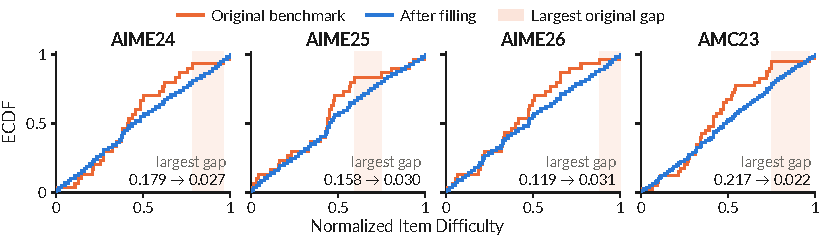
\includegraphics[width=\linewidth]{Fig/ecdf_paper.pdf}
      \vspace{-4mm}

    \caption{\textbf{四个基准在缺口填补前后的难度分布。} 橙色与蓝色曲线分别表示应用 \textsc{BenchFill} 之前与之后的经验难度分布。阴影区域标出原始的最大覆盖缺口。标注数值给出填补前后的最大间隔。}
    \label{fig:curated_benchmarks}
        \vspace{-5mm}
\end{figure*}

\subsection{经过整理的缺口填补基准}
\label{sec:curated_benchmarks}

为给未来模型与训练方法的更可靠评测提供社区资源，我们进一步将 \textsc{BenchFill} 应用于四个覆盖缺口显著、被广泛使用的数学基准，构造其缺口填补变体：AMC23、AIME24、AIME25 与 AIME26。我们将这些基准分别从 40、30、30 与 30 道题扩展到 80、50、52 与 53 道题。所有生成题目都经过人工审核，低质量或错误的题目被丢弃。我们将所得变体发布为 \textbf{AMC23-BenchFill}、\textbf{AIME24-BenchFill}、\textbf{AIME25-BenchFill} 与 \textbf{AIME26-BenchFill}\footnote{\url{https://huggingface.co/datasets/Yifan99/BenchFill}}。如图~\ref{fig:curated_benchmarks} 所示，这些变体大幅缩小了原始的最大覆盖缺口，并使经验难度分布更接近均匀分布，从而在难度谱上提供更全面的覆盖。


% \begin{table*}[t]
% \centering
% \caption{\textbf{Gap-filling results.}
% Target Dev. denotes the mean absolute deviation between the selected item difficulty and the target difficulty over three filled gaps. Top-5 Sum denotes the total size of the five largest adjacent difficulty gaps. Lower is better for both metrics.}
% \label{tab:gap_filling_results}
% \small

% \begin{minipage}[t]{0.49\linewidth}
% \vspace{0pt}
% \centering
% \resizebox{\linewidth}{!}{
% \begin{tabular}{lccccc}
% \toprule
% \textbf{Benchmark} 
% & \multicolumn{2}{c}{\textbf{Target Dev.} $\downarrow$}
% & \multicolumn{3}{c}{\textbf{Top-5 Sum} $\downarrow$} \\
% \cmidrule(lr){2-3}
% \cmidrule(lr){4-6}
% & \textbf{Rand.} & \textbf{\textsc{BenchFill}}
% & \textbf{Before} & \textbf{Rand.} & \textbf{\textsc{BenchFill}} \\
% \midrule
% AIME24 &  & 0.009 & 0.502 &  & 0.411 \\
% AIME25 &  & 0.007 & 0.492 &  & 0.355 \\
% AIME26 &  & 0.004 & 0.507 &  & 0.413 \\
% AMC23  &  & 0.005 & 0.528 &  & 0.397 \\
% \bottomrule
% \end{tabular}
% }
% \end{minipage}
% \hfill
% \begin{minipage}[t]{0.49\linewidth}
% \vspace{0pt}
% \centering
% \resizebox{\linewidth}{!}{
% \begin{tabular}{lccccc}
% \toprule
% \textbf{Benchmark} 
% & \multicolumn{2}{c}{\textbf{Target Dev.} $\downarrow$}
% & \multicolumn{3}{c}{\textbf{Top-5 Sum} $\downarrow$} \\
% \cmidrule(lr){2-3}
% \cmidrule(lr){4-6}
% & \textbf{Rand.} & \textbf{\textsc{BenchFill}}
% & \textbf{Before} & \textbf{Rand.} & \textbf{\textsc{BenchFill}} \\
% \midrule
% Gaokao2023en &  & 0.009 & 0.183 &  & 0.136 \\
% BBH-3 objects &  & 0.006 & 0.354 &  & 0.297 \\
% MMLU-Pro-Biology &  & 0.002 & 0.176 &  & 0.142 \\
% IFEval &  & 0.005 & 0.190 &  & 0.158 \\
% \bottomrule
% \end{tabular}
% }
% \end{minipage}

% \end{table*}

\section{相关工作}

\paragraph{基准评测的科学。}
近期一系列工作将注意力从提高排行榜分数，转向审视基准分数本身是否提供可靠的科学证据。除数据污染之外——即基准测试题出现在模型训练数据中、从而可能抬高评测分数~\cite{oren2024proving,sun2025emperor,zhu2024dynamic}——已有研究表明，基准结果对解码、提示与实现细节敏感~\cite{hochlehnert2025sober}，并且对表面措辞或数据集缺陷十分脆弱~\cite{mousavi2026garbage}。另有工作从信号与噪声的角度研究评测可靠性~\cite{heineman2025signal}，或提出更广泛的基准质量准则，并表明广泛使用的基准在质量上差异很大~\cite{qian2026benchmark}。我们的工作补充了这些努力：将基准表述为难度上的经验测度，从而能够严格形式化测度失配与覆盖缺口。

\paragraph{IRT 及其应用。} IRT 起源于心理测量学，是教育与心理测量的一个框架~\cite{embretson2013item,lord2012applications}。在 NLP 中，\cite{lalor2016building} 将 IRT 引入系统评测，\cite{rodriguez2021evaluation} 将这一视角扩展到排行榜分析。此后，IRT 成为 LLM 基准中难度感知评测的广泛基础。Easy2Hard-Bench~\cite{ding2024easy2hard} 使用 IRT 为基准题目赋予标准化的连续难度标签；它还将这些标签与人类成对判断进行验证，并报告其一致性优于基于 GPT-4 的难度标注器。\cite{zhou2026lost} 使用基于 IRT 的框架分析现有 LLM 基准的测量质量。
% Beyond benchmark analysis, IRT has also been used for efficient evaluation~\cite{kipnis2024metabench,polo2024tinybenchmarks,zhang2025benchmark}, whose goal is to preserve the information of much larger benchmarks using far fewer evaluation items, and for adaptive testing, whose goal is to select the most informative items for each model based on its estimated ability during evaluation~\cite{hofmann2025fluid}.

% \paragraph{Rethinking benchmark analysis.} A recent line of work has shifted attention from improving leaderboard scores to examining whether benchmark scores themselves provide reliable scientific evidence. \cite{hochlehnert2025sober} shows that reasoning benchmark results can vary substantially under seemingly minor evaluation choices, such as decoding settings, prompt format, or implementation details, and calls for more standardized and reproducible evaluation. \cite{heineman2025signal} studies benchmark quality through the lens of signal, the ability to separate models, and noise, the instability induced by random variation, and analyzes practical ways to improve reliability. \cite{mousavi2026garbage} further shows that reasoning benchmark scores can be brittle to surface wording and dataset flaws, motivating more diagnostic and interpretable evaluation. \cite{qian2026benchmark} proposes explicit criteria for benchmark quality, including ranking consistency, discriminability, and capability alignment, and shows that widely used benchmarks vary substantially along these dimensions. Our work differs by formulating a benchmark as an empirical measure over the difficulty axis, which enables us to analyze how measure mismatch distorts aggregate score comparisons and how discrete coverage gaps hide localized model improvements.


\section{结论}

本文将每个基准视为难度上的一个经验测度。这一视角使我们能够形式化测度失配与覆盖缺口，并由此得到理论结果与实用诊断。
% We encourage benchmark designers and users to use these diagnostics to inspect the difficulty structure of their benchmarks. 
我们相信，这种经验测度观点有潜力开辟新的途径，用以严格研究并重新思考基准评测。



\section*{致谢}
我们感谢 Modal 通过 Modal for Academics 计算资助支持本研究。我们亦感谢 Sirui Chen 与 Junsheng Huang 富有洞见的讨论和宝贵反馈，这些讨论与反馈帮助改进了本工作。



\bibliographystyle{plain}
\small\bibliography{neurips_2026}





%%%%%%%%%%%%%%%%%%%%%%%%%%%%%%%%%%%%%%%%%%%%%%%%%%%%%%%%%%%%

\appendix
\newpage
\section{讨论}


\subsection{更广泛的影响}
\label{sec:app_impact}

本工作旨在提高基准评测的可靠性与透明度。通过诊断分布失配与覆盖缺口，我们的方法可以帮助研究者更好地理解基准分数何时为模型比较和训练进展监测提供忠实证据。更可靠的评测可能支持更透明的模型比较和更有依据的基准设计。由于本工作聚焦于基准分析，而非模型部署或数据收集，我们预计不会产生直接的负面社会影响。

\subsection{局限性与未来工作}
\label{sec:app_limitation}

本工作建立基准评测的测度论观点，并用它刻画两个核心问题：测度失配与覆盖缺口。我们的目标不是穷尽这一观点的全部后果，而是表明基准评测可以通过基准所诱导的经验难度测度的几何来研究。我们相信，这一视角为研究基准评测开辟了更广阔的方向：额外的基准失效与设计目标都可以表述为所诱导难度测度的性质。

此外，我们当前的框架主要是事后的：给定一个已有基准，我们估计其难度分布，诊断测度失配与覆盖缺口，并通过有针对性的题目插入来缩小显著缺口。一个自然的下一步是把这一视角推进到基准构造阶段本身。与其只在基准建成之后审计失配与覆盖，基准开发者可以从一开始就主动设计所诱导的难度结构，目标是使基准测度与预期评测目标对齐，同时沿难度轴保持高局部分辨率。我们将此视为难度感知基准设计的一个有前景的方向。

\subsection{扩展相关工作}

\paragraph{难度估计。} 先前工作常常从人类判断或基准元数据中导出难度标签。例如，MATH~\cite{hendrycks2021measuring} 用五个难度级别标注问题，GPQA~\cite{rein2024gpqa} 收集事后的专家难度评分，LingOly~\cite{bean2024lingoly} 包含五个级别的人类难度。此类标签在大规模上获取代价高昂，而且它们主要反映人类感知的难度，而不是当前 LLM 在这些题目上表现出的难度。近期工作探索了其他估计策略。\citep{zhu2025llm} 从隐藏表示估计 LLM 所感知的题目难度。\cite{ballon2025estimating} 让 LLM 做成对难度判断，并用 Bradley–Terry 分数加以汇总。EIP~\cite{zhang2026rankllm} 则从模型–题目二部图上观测到的成功与失败，联合推断题目难度与模型能力。作为补充，LoRe~\cite{zhang2025reasoning} 研究内在问题复杂度，其定义为解决问题所需的最少计算步数。
在这些方法中，IRT 仍是难度感知评测的常见基础，因为它提供了一个有原则的概率框架，可以直接从响应数据联合建模题目难度与模型能力~\cite{chen2025item}。
% \subsection{Benchmark size and Max Gap}
% Max Gap is affected by benchmark size, since smaller benchmarks naturally tend to have larger adjacent gaps. This dependence should be interpreted as a real limitation of small benchmarks rather than merely a nuisance to normalize away. Even when a large gap is expected from finite sample size, it still represents an uncovered difficulty interval; by Theorem~\ref{thm:max-gap-detection-boundary}, localized improvements within such an interval may be undetectable in the worst case. 

\section{理论结果与证明}
\label{sec:app_proof}

\subsection{测度失配}
\label{sec:app_proof_mismatch}

我们首先重述定理~\ref{thm:w1_rank_stability} 并给出相应证明。

\begin{theorem}[分布失配控制分数扭曲与排名稳定性]
设性能差函数 $\Delta$ 是 $L$-Lipschitz 的，即
\[
|\Delta(z)-\Delta(y)| \le L |z-y|,
\qquad \forall z,y \in [0,1].
\]
则
\[
\bigl|D_B(\theta',\theta) - D_\mu(\theta',\theta)\bigr|
\le
L\, W_1(\nu_B,\mu).
\]
因此，若
\[
|D_\mu(\theta',\theta)| > L\, W_1(\nu_B,\mu),
\]
则
\[
\operatorname{sign}\bigl(D_B(\theta',\theta)\bigr)
=
\operatorname{sign}\bigl(D_\mu(\theta',\theta)\bigr),
\]
从而基准所诱导的排序与目标排序一致，即不会发生排名翻转。
\end{theorem}

\begin{proof}
任取耦合 $\pi \in \Pi(\nu_B,\mu)$。由于 $\pi$ 的边缘分布为 $\nu_B$ 与 $\mu$，可以写成
\[
D_B(\theta',\theta) - D_\mu(\theta',\theta)
=
\int \Delta(z)\, d\nu_B(z) - \int \Delta(y)\, d\mu(y)
=
\int_{[0,1]^2} \bigl(\Delta(z)-\Delta(y)\bigr)\, d\pi(z,y).
\]
取绝对值并利用 $\Delta$ 的 Lipschitz 性质，得到
\[
\bigl|D_B(\theta',\theta) - D_\mu(\theta',\theta)\bigr|
\le
\int_{[0,1]^2} |\Delta(z)-\Delta(y)|\, d\pi(z,y)
\le
L \int_{[0,1]^2} |z-y|\, d\pi(z,y).
\]
由于这对每个耦合 $\pi \in \Pi(\nu_B,\mu)$ 都成立，对 $\pi$ 取下确界得到
\[
\bigl|D_B(\theta',\theta) - D_\mu(\theta',\theta)\bigr|
\le
L\, W_1(\nu_B,\mu).
\]

若 $D_\mu(\theta',\theta) > 0$，则
\[
D_B(\theta',\theta)
\ge
D_\mu(\theta',\theta) - \bigl|D_B(\theta',\theta) - D_\mu(\theta',\theta)\bigr|
\ge
D_\mu(\theta',\theta) - L\,W_1(\nu_B,\mu)
>
0.
\]
因此 $D_B(\theta',\theta) > 0$。情形 $D_\mu(\theta',\theta) < 0$ 是对称的。故 $D_B(\theta',\theta)$ 与 $D_\mu(\theta',\theta)$ 必须同号，从而不会发生排名翻转。
\end{proof}


\paragraph{重复采样下的有限样本评测。}
实践中，条件均值 $s_\theta(z)$ 并不能被直接观测。相反，基准分数由模型输出的有限次重复样本估计。对难度水平为 $z_i$ 的第 $i$ 道基准题，以及每次独立试验 $r \in \{1,\dots,k\}$，令
\[
Y_{i,r}^{\theta} \in [0,1]
\]
表示模型 $\theta$ 在第 $r$ 次样本上的观测分数，且
\[
\mathbb{E}\!\left[Y_{i,r}^{\theta}\mid z_i\right] = s_\theta(z_i).
\]
定义 $k$ 样本基准分数为
\[
\widehat{S}_{B,k}(\theta)
:=
\frac{1}{nk}\sum_{i=1}^n \sum_{r=1}^k Y_{i,r}^{\theta},
\]
相应的观测性能差为
\[
\widehat{D}_{B,k}(\theta',\theta)
:=
\widehat{S}_{B,k}(\theta')-\widehat{S}_{B,k}(\theta).
\]

\begin{theorem}[重复采样下的有限样本分数扭曲与排序稳定性]
\label{thm:noisy_rank_stability}
设性能差函数 $\Delta$ 是 $L$-Lipschitz 的。假设在给定难度水平 $z_1,\dots,z_n$ 的条件下，随机变量族
\[
\left\{Y_{i,r}^{\theta},\, Y_{i,r}^{\theta'}\right\}_{i=1,\dots,n;\, r=1,\dots,k}
\]
相互独立，且每个变量取值于 $[0,1]$。则对任意 $\delta \in (0,1)$，以至少 $1-\delta$ 的概率，有
\[
\bigl|\widehat{D}_{B,k}(\theta',\theta)-D_\mu(\theta',\theta)\bigr|
\le
L\,W_1(\nu_B,\mu)
+
\sqrt{\frac{2\log(2/\delta)}{nk}}.
\]
因此，若
\[
|D_\mu(\theta',\theta)|
>
L\,W_1(\nu_B,\mu)
+
\sqrt{\frac{2\log(2/\delta)}{nk}},
\]
则以至少 $1-\delta$ 的概率，有
\[
\operatorname{sign}\!\bigl(\widehat{D}_{B,k}(\theta',\theta)\bigr)
=
\operatorname{sign}\!\bigl(D_\mu(\theta',\theta)\bigr),
\]
从而不会发生观测到的排名翻转。
\end{theorem}

\begin{proof}
我们首先将误差分解为
\[
\widehat{D}_{B,k}(\theta',\theta)-D_\mu(\theta',\theta)
=
\Bigl(\widehat{D}_{B,k}(\theta',\theta)-D_B(\theta',\theta)\Bigr)
+
\Bigl(D_B(\theta',\theta)-D_\mu(\theta',\theta)\Bigr).
\]
因此，
\[
\bigl|\widehat{D}_{B,k}(\theta',\theta)-D_\mu(\theta',\theta)\bigr|
\le
\bigl|\widehat{D}_{B,k}(\theta',\theta)-D_B(\theta',\theta)\bigr|
+
\bigl|D_B(\theta',\theta)-D_\mu(\theta',\theta)\bigr|.
\]

第二项是确定性的，并且由定理~\ref{thm:w1_rank_stability}，满足
\[
\bigl|D_B(\theta',\theta)-D_\mu(\theta',\theta)\bigr|
\le
L\,W_1(\nu_B,\mu).
\]

剩下的是界定第一项。定义
\[
Z_{i,r}
:=
Y_{i,r}^{\theta'}-Y_{i,r}^{\theta}.
\]
由于 $Y_{i,r}^{\theta'}, Y_{i,r}^{\theta}\in[0,1]$，我们有
\[
Z_{i,r}\in[-1,1].
\]
此外，在给定 $z_i$ 的条件下，
\[
\mathbb{E}[Z_{i,r}\mid z_i]
=
\mathbb{E}[Y_{i,r}^{\theta'}\mid z_i]
-
\mathbb{E}[Y_{i,r}^{\theta}\mid z_i]
=
s_{\theta'}(z_i)-s_\theta(z_i)
=
\Delta(z_i).
\]
因此
\[
\widehat{D}_{B,k}(\theta',\theta)-D_B(\theta',\theta)
=
\frac{1}{nk}\sum_{i=1}^n \sum_{r=1}^k \Bigl(Z_{i,r}-\Delta(z_i)\Bigr).
\]
在给定 $z_1,\dots,z_n$ 的条件下，变量 $\{Z_{i,r}\}$ 相互独立，且每个都落在 $[-1,1]$ 中。对任意 $t>0$，条件地应用 Hoeffding 不等式得到
\[
\mathbb{P}\!\left(
\left.
\bigl|\widehat{D}_{B,k}(\theta',\theta)-D_B(\theta',\theta)\bigr|
\ge t
\ \right|\ z_1,\dots,z_n
\right)
\le
2\exp\!\left(-\frac{nk\,t^2}{2}\right).
\]
取
\[
t=\sqrt{\frac{2\log(2/\delta)}{nk}}
\]
则以至少 $1-\delta$ 的概率给出
\[
\bigl|\widehat{D}_{B,k}(\theta',\theta)-D_B(\theta',\theta)\bigr|
\le
\sqrt{\frac{2\log(2/\delta)}{nk}}.
\]
将该界与上面的确定性界合并，即证
\[
\bigl|\widehat{D}_{B,k}(\theta',\theta)-D_\mu(\theta',\theta)\bigr|
\le
L\,W_1(\nu_B,\mu)
+
\sqrt{\frac{2\log(2/\delta)}{nk}}
\]
以至少 $1-\delta$ 的概率成立。

对第二个结论，若
\[
|D_\mu(\theta',\theta)|
>
L\,W_1(\nu_B,\mu)
+
\sqrt{\frac{2\log(2/\delta)}{nk}},
\]
则上述不等式意味着 $\widehat{D}_{B,k}(\theta',\theta)$ 不能越过零，因此它必须与 $D_\mu(\theta',\theta)$ 同号。故不会发生观测到的排名翻转。
\end{proof}

\paragraph{无先验信息时，均匀分布作为有原则的目标分布。}

下面的结果将均匀分布形式化为一种有原则的默认目标：当对性能差沿难度轴出现的位置没有先验知识时。我们考虑一种不可知设定，其中带符号的性能差 $\Delta$ 在 $[0,1]$ 上具有固定的平均水平 $\rho$，但其位置除此之外不受限制。对候选目标分布 $\mu$，量 $V_\rho(\mu)$ 衡量在 $\mu$ 下最坏情形所保留的差的大小。下面的定理表明，均匀分布是在最坏情形下仍保留完整平均差 $\rho$ 的唯一选择。

\begin{theorem}[完全不确定下，均匀目标是唯一的极大极小选择]
令
\[
\mathcal F_\rho
:=
\left\{
\Delta:[0,1]\to[-1,1]\ \text{可测} :
\int_0^1 \Delta(z)\,dz = \rho
\right\},
\qquad
V_\rho(\mu)
:=
\inf_{\Delta\in\mathcal F_\rho}\int \Delta(z)\,d\mu(z),
\]
其中 $\rho\in(-1,1)$ 且 $\mu\in\mathcal P([0,1])$。则
\[
\sup_{\mu\in\mathcal P([0,1])} V_\rho(\mu)=\rho\]
且唯一的最大化子是均匀分布 $\lambda=\mathrm{Unif}[0,1]$。
\end{theorem}

\begin{proof}
令
\[
\beta := \frac{1+\rho}{2}\in(0,1).
\]
对任意可测函数 $\Delta:[0,1]\to[-1,1]$，定义
\[
G(z):=\frac{\Delta(z)+1}{2}.
\]
则 $G:[0,1]\to[0,1]$ 可测，且
\[
\int_0^1 G(z)\,dz
=
\frac{1}{2}\int_0^1 \Delta(z)\,dz+\frac{1}{2}.
\]
因此，$\Delta \in \mathcal F_\rho$ 当且仅当
\[
G:[0,1]\to[0,1]
\qquad\text{且}\qquad
\int_0^1 G(z)\,dz=\beta.
\]
于是，对任意 $\mu\in\mathcal P([0,1])$，
\[
V_\rho(\mu)
=
\inf_{\Delta\in\mathcal F_\rho}\int \Delta(z)\, d\mu(z)
=
\inf_{G:\,[0,1]\to[0,1],\, \int_0^1 G(z)\,dz=\beta}
\int (2G(z)-1)\, d\mu(z).
\]
由于 $\mu$ 是概率测度，
\[
V_\rho(\mu)
=
2 \inf_{G:\,[0,1]\to[0,1],\, \int_0^1 G(z)\,dz=\beta}
\int G(z)\, d\mu(z)-1.
\]
定义
\[
U_\beta(\mu)
:=
\inf_{G:\,[0,1]\to[0,1],\, \int_0^1 G(z)\,dz=\beta}
\int G(z)\, d\mu(z).
\]
则
\[
V_\rho(\mu)=2U_\beta(\mu)-1.
\]

现在刻画 $\sup_{\mu\in\mathcal P([0,1])} U_\beta(\mu)$。

首先，若 $\mu=\lambda=\mathrm{Unif}[0,1]$，则对每个可允许的 $G$，
\[
\int G(z)\, d\mu(z)
=
\int_0^1 G(z)\,dz
=
\beta,
\]
故
\[
U_\beta(\lambda)=\beta.
\]
因此
\[
\sup_{\mu\in\mathcal P([0,1])} U_\beta(\mu)\ge \beta.
\]

接下来固定任意 $\mu\in\mathcal P([0,1])$。由 Lebesgue 分解定理，可以写成
\[
\mu = f(z)\,dz + \mu_s,
\]
其中 \(f\ge 0\) 可积且 \(\mu_s \perp dz\)。令
\[
m := \int_0^1 f(z)\,dz = \mu_{\mathrm{ac}}([0,1]) \le 1.
\]
由于 \(\mu_s\) 关于 Lebesgue 测度奇异，存在可测集 \(N\subseteq[0,1]\) 使得
\[
|N|=0
\qquad\text{且}\qquad
\mu_s([0,1]\setminus N)=0.
\]
于是，对任意在 \(N\) 上取零的可允许 \(G\)，我们有
\[
\int G(z)\, d\mu_s(z)=0.
\]
因此，
\[
U_\beta(\mu)
\le
\inf_{\substack{0\le G\le 1,\ \int_0^1 G(z)\,dz=\beta,\\ G=0\ \text{在 }N\text{ 上}}}
\int_0^1 G(z) f(z)\,dz.
\]
由于 \(N\) 的 Lebesgue 测度为零，附加约束“\(G=0\) 在 \(N\) 上”不影响下确界，故
\[
U_\beta(\mu)
\le
\inf_{0\le G\le 1,\ \int_0^1 G(z)\,dz=\beta}
\int_0^1 G(z) f(z)\,dz.
\]
由浴缸原理，右端等于
\[
\int_0^\beta f^\uparrow(u)\,du,
\]
其中 \(f^\uparrow\) 是 \(f\) 的非降重排。由于 \(f^\uparrow\) 非降且 $\beta \in (0,1)$，
\[
\frac{1}{\beta}\int_0^\beta f^\uparrow(u)\,du
\le
\int_0^1 f^\uparrow(u)\,du
=
\int_0^1 f(z)\,dz \le 1.
\]
因此
\[
U_\beta(\mu)\le \beta.
\]
由于这对每个 \(\mu\in\mathcal P([0,1])\) 都成立，我们得到
\[
\sup_{\mu\in\mathcal P([0,1])} U_\beta(\mu)=\beta.
\]
从而，
\[
\sup_{\mu\in\mathcal P([0,1])} V_\rho(\mu)
=
2\sup_{\mu\in\mathcal P([0,1])} U_\beta(\mu)-1
=
2\beta-1
=
\rho.
\]

剩下的是证明唯一性。设 \(V_\rho(\mu)=\rho\)。则必然有
\[
U_\beta(\mu)=\beta.
\]
由上面的论证，这蕴含
\[
\int_0^\beta f^\uparrow(u)\,du=\beta
\qquad\text{且}\qquad
\int_0^1 f(z)\,dz=1.
\]
第二个条件蕴含 \(\mu_s=0\)，因此 \(\mu\) 关于密度 \(f\) 绝对连续。此外，
\[
\frac{1}{\beta}\int_0^\beta f^\uparrow(u)\,du = 1
\]
等于 \(f^\uparrow\) 在整个区间 \([0,1]\) 上的平均值，该平均值同样为 \(1\)。由于 \(f^\uparrow\) 非降，这仅当
\[
f^\uparrow(u)=1
\qquad\text{对几乎处处 }u\in[0,1].
\]
因此对几乎处处 \(z\in[0,1]\) 有 \(f(z)=1\)，从而 \(\mu=\lambda\)。这证明了唯一性。
\end{proof}

\subsection{覆盖缺口}
\label{sec:app_proof_missed}

为分析局部改进能否从基准评测中被检测出来，我们将该问题表述为比较改进前后两条性能曲线的假设检验。我们考虑一对一般的改进前与改进后性能曲线
\[
s^{-},s^{+}:[0,1]\to[0,1].
\]
这里，$s^{-}(z)$ 与 $s^{+}(z)$ 分别表示改进前与改进后在难度水平 $z$ 上的期望模型性能（例如 pass@1）。它们的差为
\[
\Delta(z):=s^{+}(z)-s^{-}(z).
\]

对第 \(i\) 道基准题以及每次试验 \(r\in\{1,\dots,k\}\)，令
\[
Y_{i,r}^{-}\sim \mathrm{Bernoulli}(s^{-}(z_i)),
\qquad
Y_{i,r}^{+}\sim \mathrm{Bernoulli}(s^{+}(z_i)).
\]
我们假设，在给定难度水平与性能曲线的条件下，所有变量
\[
\{Y_{i,r}^{-},Y_{i,r}^{+}\}_{i=1,\dots,n;\ r=1,\dots,k}
\]
相互独立。
定义
\[
\widehat{S}_{B,k}(s^-)
:=
\frac{1}{nk}\sum_{i=1}^n\sum_{r=1}^k Y_{i,r}^{-},
\qquad
\widehat{S}_{B,k}(s^+)
:=
\frac{1}{nk}\sum_{i=1}^n\sum_{r=1}^k Y_{i,r}^{+},
\]
以及
\[
\widehat{D}_{B,k}(s^+,s^-)
:=
\widehat{S}_{B,k}(s^+)-\widehat{S}_{B,k}(s^-).
\]

固定 $w\in(0,1]$ 与 $a\in(0,1]$。我们定义局部化备择类
\[
\mathcal H_1(w,a)
:=
\Bigl\{
(s^-,s^+):
\exists \text{ 区间 } I\subset[0,1],\ |I|=w,
\ \text{使得 } s^{+}(z)-s^{-}(z)\ge a \ \ \forall z\in I
\Bigr\}.
\]

这里，参数 $(w,a)$ 刻画改进模式：
$w$ 表示改进发生的难度区域宽度，$a$ 表示该区域内改进的最小幅度。

原假设类为
\[
\mathcal H_0
:=
\{(s^-,s^+): s^-=s^+\}.
\]
于是我们考虑检验问题
\[
H_0:\ (s^-,s^+)\in\mathcal H_0
\qquad\text{对}\qquad
H_1:\ (s^-,s^+)\in\mathcal H_1(w,a).
\]

这一表述刻画的问题是：基准能否可靠地检测宽度为 $w$、幅度至少为 $a$ 的有意义局部改进。

一个（可能随机化的）检验 $\phi$ 的水平至多为 $\alpha\in(0,1)$，如果
\[
\sup_{(s^-,s^+)\in\mathcal H_0}\mathbb E_{s^-,s^+}[\phi]\le \alpha.
\]
它在 $\mathcal H_1(w,a)$ 上的最坏情形功效为
\[
\inf_{(s^-,s^+)\in\mathcal H_1(w,a)} \mathbb E_{s^-,s^+}[\phi].
\]
我们将极小极大最坏情形功效定义为
\[
\Pi_\alpha^*(B;w,a,k)
:=
\sup_{\phi:\ \sup_{(s^-,s^+)\in\mathcal H_0}\mathbb E_{s^-,s^+}[\phi]\le \alpha}
\ \inf_{(s^-,s^+)\in\mathcal H_1(w,a)} \mathbb E_{s^-,s^+}[\phi].
\]

\begin{theorem}[最大间隔作为精确的渐近极小极大检测边界]
固定 $\alpha\in(0,1)$ 与 $a\in(0,1]$。

\begin{enumerate}
\item 对每个 $k\in\mathbb N$，若 $w\le G(B)$，则
\[
\Pi_\alpha^*(B;w,a,k)=\alpha.
\]

\item 若 $w>G(B)$，则
\[
\lim_{k\to\infty}\Pi_\alpha^*(B;w,a,k)=1.
\]
\end{enumerate}

因此，$G(B)$ 是基准 $B$ 下区间局部化差异的精确渐近极小极大检测边界。
\end{theorem}

\begin{proof}
我们分别证明两部分。

\smallskip
\noindent\textbf{第一部分：若 $w\le G(B)$，则 $\Pi_\alpha^*(B;w,a,k)=\alpha$。}

由最大间隔的定义，存在指标 $j\in\{0,\dots,n\}$ 使得
\[
z_{(j+1)}-z_{(j)}\ge w.
\]
令
\[
J := (z_{(j)},z_{(j+1)}).
\]
由于
\[
|J| = z_{(j+1)} - z_{(j)} \ge w,
\]
我们可以选取一个区间
\[
I \subseteq J
\qquad\text{使得}\qquad
|I| = w .
\]
任取 \(c\in[0,1-a]\)，并定义
\[
s^{-,\star}(z)\equiv c,
\qquad
s^{+,\star}(z):=c+a\,\mathbf 1\{z\in I\}.
\]
由于 \(c\in[0,1-a]\) 且 \(a\in(0,1]\)，$s^{-,\star}$ 与 $s^{+,\star}$ 的取值都在 \([0,1]\) 中。此外，
\[
s^{+,\star}(z)-s^{-,\star}(z)=a
\qquad\forall z\in I,
\]
故
\[
(s^{-,\star},s^{+,\star})\in\mathcal H_1(w,a).
\]

因为区间 \(I\) 不含任何基准点，对每个 \(i=1,\dots,n\) 我们有
\[
s^{-,\star}(z_i)=c,
\qquad
s^{+,\star}(z_i)=c.
\]
因此，在 \((s^{-,\star},s^{+,\star})\) 下，基准观测与原假设对
\[
(\bar s,\bar s)\in\mathcal H_0
\qquad\text{其中}\qquad
\bar s(z)\equiv c
\]
具有完全相同的联合分布。
事实上，在每个被观测的基准点 \(z_i\) 上，改进前与改进后的 Bernoulli 成功概率都等于 \(c\)。

现令 $\phi$ 为任意水平至多为 $\alpha$ 的检验。则
\[
\mathbb E_{s^{-,\star},s^{+,\star}}[\phi]
=
\mathbb E_{\bar s,\bar s}[\phi]
\le
\sup_{(s^-,s^+)\in\mathcal H_0}\mathbb E_{s^-,s^+}[\phi]
\le \alpha.
\]
因此
\[
\inf_{(s^-,s^+)\in\mathcal H_1(w,a)}\mathbb E_{s^-,s^+}[\phi]
\le
\mathbb E_{s^{-,\star},s^{+,\star}}[\phi]
\le \alpha.
\]
对所有水平 $\alpha$ 的检验取上确界，得到
\[
\Pi_\alpha^*(B;w,a,k)\le \alpha.
\]

对反向不等式，考虑与数据无关、以概率 $\alpha$ 拒绝的平凡随机化检验。它的水平恰好为 $\alpha$，并且对每个备择其功效也恰好为 $\alpha$。因此
\[
\Pi_\alpha^*(B;w,a,k)\ge \alpha.
\]
合并两个不等式，我们得到
\[
\Pi_\alpha^*(B;w,a,k)=\alpha.
\]

\smallskip
\noindent\textbf{第二部分：若 $w>G(B)$，则 $\lim_{k\to\infty}\Pi_\alpha^*(B;w,a,k)=1$。}

我们构造一个显式的水平 $\alpha$ 检验，其最坏情形功效在 $k\to\infty$ 时趋于 $1$。

对每个基准点 $z_i$，定义经验差
\[
\widehat{\Delta}_{i,k}
:=
\frac{1}{k}\sum_{r=1}^k\bigl(Y_{i,r}^{+}-Y_{i,r}^{-}\bigr).
\]
考虑最大值检验
\[
\phi_{\max}
:=
\mathbf 1\left\{
\max_{1\le i\le n}\widehat{\Delta}_{i,k}
>
t_{k,\alpha}
\right\},
\qquad
t_{k,\alpha}
:=
\sqrt{\frac{2\log(n/\alpha)}{k}}.
\]

我们首先验证 $\phi_{\max}$ 的水平至多为 $\alpha$。在任意原假设对 $(s,s)\in\mathcal H_0$ 下，对每个固定的 $i$ 与 $r$，
\[
Y_{i,r}^{+}-Y_{i,r}^{-}\in[-1,1],
\qquad
\mathbb E_{s,s}[Y_{i,r}^{+}-Y_{i,r}^{-}]=0,
\]
并且这些随机变量关于 $r$ 相互独立。因此，由 Hoeffding 不等式，
\[
\mathbb P_{s,s}\!\left(\widehat{\Delta}_{i,k}>t\right)
\le
\exp\!\left(-\frac{k t^2}{2}\right).
\]
对 $i=1,\dots,n$ 应用并集界，得到
\[
\mathbb P_{s,s}(\phi_{\max}=1)
=
\mathbb P_{s,s}\!\left(\max_{1\le i\le n}\widehat{\Delta}_{i,k}>t_{k,\alpha}\right)
\le
\sum_{i=1}^n
\mathbb P_{s,s}\!\left(\widehat{\Delta}_{i,k}>t_{k,\alpha}\right)
\le
n\exp\!\left(-\frac{k t_{k,\alpha}^2}{2}\right)
=
\alpha.
\]
由于该界对 $(s,s)\in\mathcal H_0$ 一致成立，检验 $\phi_{\max}$ 的水平至多为 $\alpha$。

接下来固定任意备择对 $(s^-,s^+)\in\mathcal H_1(w,a)$。由定义，存在区间 $I\subset[0,1]$ 满足 $|I|=w$，使得
\[
s^+(z)-s^-(z)\ge a,
\qquad \forall z\in I.
\]
因为 $w>G(B)$，任何长度为 $w$ 的区间都不能与所有基准点不相交。因此，至少存在一个基准指标 $i^\star$ 使得
\[
z_{i^\star}\in I.
\]
对该指标，我们有
\[
\mathbb E_{s^-,s^+}[\widehat{\Delta}_{i^\star,k}]
=
s^+(z_{i^\star})-s^-(z_{i^\star})
\ge a.
\]

再次由 Hoeffding 不等式，对任意 $t\in\mathbb R$，
\[
\mathbb P_{s^-,s^+}\!\left(
\widehat{\Delta}_{i^\star,k}\le t
\right)
\le
\exp\!\left(
-\frac{k}{2}\bigl(a-t\bigr)_+^2
\right),
\]
其中 $(u)_+:=\max\{u,0\}$。取 $t=t_{k,\alpha}$ 得到
\[
\mathbb P_{s^-,s^+}\!\left(
\widehat{\Delta}_{i^\star,k}\le t_{k,\alpha}
\right)
\le
\exp\!\left(
-\frac{k}{2}\bigl(a-t_{k,\alpha}\bigr)_+^2
\right).
\]
由于事件
\[
\left\{\widehat{\Delta}_{i^\star,k}>t_{k,\alpha}\right\}
\]
蕴含
\[
\left\{\max_{1\le i\le n}\widehat{\Delta}_{i,k}>t_{k,\alpha}\right\},
\]
我们得到
\[
\mathbb P_{s^-,s^+}(\phi_{\max}=1)
\ge
\mathbb P_{s^-,s^+}\!\left(
\widehat{\Delta}_{i^\star,k}>t_{k,\alpha}
\right)
\ge
1-
\exp\!\left(
-\frac{k}{2}\bigl(a-t_{k,\alpha}\bigr)_+^2
\right).
\]
该下界对所有 $(s^-,s^+)\in\mathcal H_1(w,a)$ 一致成立，故
\[
\inf_{(s^-,s^+)\in\mathcal H_1(w,a)}
\mathbb E_{s^-,s^+}[\phi_{\max}]
\ge
1-
\exp\!\left(
-\frac{k}{2}\bigl(a-t_{k,\alpha}\bigr)_+^2
\right).
\]
由于极小极大功效至少是任一具体水平 $\alpha$ 检验的最坏情形功效，
\[
\Pi_\alpha^*(B;w,a,k)
\ge
1-
\exp\!\left(
-\frac{k}{2}\bigl(a-t_{k,\alpha}\bigr)_+^2
\right).
\]
最后，因为
\[
t_{k,\alpha}
=
\sqrt{\frac{2\log(n/\alpha)}{k}}
\longrightarrow 0
\qquad\text{当 }k\to\infty,
\]
右端收敛到 $1$。由于按功效的定义有 $\Pi_\alpha^*(B;w,a,k)\le 1$，夹逼定理蕴含
\[
\lim_{k\to\infty}\Pi_\alpha^*(B;w,a,k)=1.
\]

证毕。
\end{proof}


\section{难度估计细节与补充结果}
\label{sec:app_diff_est_details}
\subsection{基准细节}
\label{sec:app_benchmark_details}
表~\ref{tab:benchmark_summary} 汇总了分析中使用的基准，包括其领域、样本数以及评测时每道题的 rollout 次数。

\begin{table}[h]
\centering
\caption{\textbf{分析中所用基准的汇总。} 为简洁起见，全文将 SWE-bench Verified (Mini) 简写为 SWE-bench-Mini，并将 BIG-Bench Hard-Logical Deduction-\{3,5,7\} objects 简写为 BBH-\{3,5,7\} objects。}
\label{tab:benchmark_summary}
\resizebox{1.0\linewidth}{!}{
\begin{tabular}{l l r r}
\toprule
\textbf{基准} & \textbf{领域} & \textbf{样本数} & \textbf{每题 rollout 数} \\
\midrule
MATH-500~\cite{lightman2023let} & 数学 & 500 & 8 \\
Minerva-Math~\cite{lewkowycz2022solving}  & 数学 & 272 & 8 \\
OlympiadBench~\cite{he2024olympiadbench} & 数学 & 675 & 8 \\
Gaokao2023en~\cite{zhang2023evaluating} & 数学 & 385 & 8 \\
AMC23~\cite{amc23} & 数学 & 40 & 32 \\
AIME24~\cite{AIME24} & 数学 & 30 & 32 \\
AIME25~\cite{AIME25} & 数学 & 30 & 32 \\
AIME26~\cite{aime26} & 数学 & 30 & 32 \\
\midrule
HumanEval~\cite{chen2021codex} & 编程 & 164 & 4 \\
MBPP+~\cite{liu2023your} & 编程 & 378 & 4 \\
\midrule
GAIA~\cite{mialon2023gaia} & 智能体任务 & 165 & 1 \\
CORE-Bench Hard
~\cite{siegel2024core} & 智能体任务 & 45 & 1 \\
SWE-bench Verified (Mini)~\cite{jimenez2023swe} & 智能体任务 & 50 & 1 \\
USACO
~\cite{shi2024can} & 智能体任务 & 307 & 1 \\
\midrule
MMLU-Pro-Biology~\cite{wang2024mmlu} & 科学 & 717 & 4 \\
MMLU-Pro-Chemistry~\cite{wang2024mmlu} & 科学 & 1132 & 4 \\
MMLU-Pro-Physics~\cite{wang2024mmlu} & 科学 & 1299 & 4 \\
GPQA-Diamond~\cite{rein2024gpqa} & 科学 & 198 & 4 \\
ScienceQA~\cite{lu2022learn} & 科学 & 4241 & 4 \\
\midrule
IFEval~\cite{zhou2023instruction} & 指令遵循 & 541 & 4 \\
\midrule
BIG-Bench Hard-Logical Deduction-3 objects~\cite{suzgun2022challenging} & 逻辑 & 250  & 4 \\
BIG-Bench Hard-Logical Deduction-5 objects~\cite{suzgun2022challenging} & 逻辑 & 250  & 4 \\
BIG-Bench Hard-Logical Deduction-7 objects~\cite{suzgun2022challenging} & 逻辑 & 250 & 4 \\
ZebraLogic~\cite{zebralogic2025} & 逻辑 & 1000 & 4 \\
\midrule
MedQA~\cite{jin2021disease} & 医学 & 1273 & 4 \\
\bottomrule
\end{tabular}
}
\end{table}

\subsection{模型选择细节}
\label{sec:app_model_details}

对非智能体任务，我们依据 Text Arena 的总体排行榜选择模型。其评测套件覆盖多种领域，包括 \texttt{Expert}、\texttt{Hard Prompts}、\texttt{Coding}、\texttt{Math}、\texttt{Creative Writing}、\texttt{Instruction Following} 与 \texttt{Longer Query}。因此总体分数为模型在广泛任务上的能力提供了合理代理。为获得能力水平多样的模型，我们按总体分数将排行榜划分为 10 个等宽层级。然后从每个层级随机选取一个模型，并额外纳入排行榜顶部与底部各一个模型。由此得到共 12 个模型，覆盖宽广的能力谱。详细模型信息汇总于表~\ref{tab:model_details}。

\begin{table}[h]
\centering
\caption{\textbf{非智能体任务所选模型汇总。}}
\label{tab:model_details}
\resizebox{0.85\linewidth}{!}{
\begin{tabular}{l l l c c}
\toprule
\textbf{模型} & \textbf{规模} & \textbf{提供方} & \textbf{Temperature} & \textbf{Top-$p$} \\
\midrule
Qwen3.5-397B-A17B & 397B & Alibaba Qwen & 0.6 & 0.95 \\
GLM-4.6  & 357B & Zhipu AI & 1.0 & 0.95 \\
GLM-4.5-Air & 110B & Zhipu AI & 0.6 & 0.95 \\
Qwen3-Next-80B-A3B-Instruct  & 80B & Alibaba Qwen & 0.7 & 0.8 \\
QwQ-32B & 32B & Alibaba Qwen & 0.6 & 0.95 \\
Olmo-3.1-32B-Think & 32B & Allen AI & 0.6 & 0.95 \\
gpt-oss-20b & 20B & OpenAI & 1.0 & 1.0 \\
phi-4 & 14B & Microsoft & 0.8 & 0.95 \\
Llama-3.1-8B-Instruct & 8B & Meta-Llama & 0.6 & 0.9 \\
vicuna-7b-v1.5 & 7B & LMSYS & 0.9 & 0.6 \\
Llama-3.2-3B-Instruct & 3B & Meta-Llama & 0.6 & 0.9 \\
SmolLM2-1.7B-Instruct & 1.7B & HuggingFaceTB & 0.7 & 0.8 \\
\bottomrule
\end{tabular}
}
\end{table}

对智能体任务，我们使用 HAL 评测平台所包含的模型。其中包括若干主要提供方的前沿专有模型，例如 Claude Sonnet~4.5、Claude Opus~4.1、GPT-5 与 Gemini 2.0 Flash。

\subsection{IRT 拟合与诊断}
\label{sec:app_irt}

为获得可靠的难度估计，我们对响应矩阵和 IRT 拟合过程都进行若干诊断检查。

\paragraph{响应矩阵诊断。}
我们用四个诊断检查每个响应矩阵。前两个，\emph{模型信息量}与\emph{题目信息量}，衡量矩阵沿模型维与题目维是否包含足够的判别信号~\cite{baker2001basics}。
% Intuitively, if most models either solve almost all items or almost none of them, or if most items are solved by nearly all models or by almost none, then the response matrix provides little signal for distinguishing weak from strong models or hard from easy items. 
后两个，\emph{模型逆序率}与\emph{题目逆序率}，衡量经验响应矩阵与 1PL-IRT 所蕴含的单调结构吻合程度~\cite{sijtsma1998nonparametric, sijtsma1996survey}。
% Intuitively, once models are ordered from weaker to stronger and items are ordered from harder to easier, a stronger model should be more likely than a weaker model to solve the same item, and an easier item should be more likely than a harder item to be solved by the same model. Inversions quantify how often these expected comparisons are violated.

形式上，对每个题目--模型对 $(i,j)$，我们将观测响应汇总为模型 $j$ 在题目 $i$ 上的经验成功率，定义为 $p_{ij}=n_{ij}^{\mathrm{correct}}/n_{ij}^{\mathrm{trials}}$。然后沿模型维与题目维汇总这些成功率：
\[
p_j=\frac{1}{|\mathcal I|}\sum_{i\in\mathcal I} p_{ij}, \qquad
p_i=\frac{1}{|\mathcal J|}\sum_{j\in\mathcal J} p_{ij},
\]
其中 $\mathcal I$ 与 $\mathcal J$ 分别表示题目集合与模型集合。我们将模型信息量定义为 $4p_j(1-p_j)$ 在模型上的平均，将题目信息量定义为 $4p_i(1-p_i)$ 在题目上的平均。其直观含义是：若许多模型几乎解出所有题目或几乎一道都解不出，则其汇总成功率饱和，对区分模型能力贡献的信息有限。当许多题目被几乎所有模型解出或几乎没有模型解出时，情况相同。相反，接近 $0.5$ 的汇总成功率信息量更大，因为它们对应既不饱和也不退化的模型或题目。因子 $4$ 将该量重新缩放到 $[0,1]$。

为评估响应矩阵是否与 1PL-IRT 所蕴含的序一致，我们首先按总体成功率对模型排序，按总体解出率对题目排序。然后计算两个逆序率。模型逆序率是有序模型对中、逐题评估时较强模型表现差于较弱模型的比例。题目逆序率是有序题目对中、逐模型评估时较易题目被解出次数少于较难题目的比例。较低的逆序率表明与 IRT 所假设的潜在序更一致。

在实验中，我们以模型信息量 $\ge 0.3$、题目信息量 $\ge 0.3$、模型逆序率 $\le 0.3$、题目逆序率 $\le 0.3$ 作为基本阈值。通过这些检查表明矩阵包含足够信号，并且与 IRT 的序假设合理一致。

\paragraph{IRT 拟合。} 我们用贝叶斯推断拟合 1PL-IRT 模型。对选择题基准，我们额外纳入一个猜测参数：
\[
\Pr(Y_{ij}=1)=g_i+(1-g_i)\sigma(\theta_j-b_i),
\]
其中 \(g_i\) 表示靠猜测答对题目 \(i\) 的机会水平概率。

模型能力 $\theta_j$ 与题目难度 $b_i$ 被赋予独立的高斯先验，
\[
\theta_j \sim \mathcal{N}(0,1), \qquad
b_i \sim \mathcal{N}(0,1).
\]
由于每个模型–题目对被评估多次，我们用二项似然建模正确回答的次数。后验推断使用 PyMC~\cite{pymc2023} 中实现的 No-U-Turn Sampler（NUTS）进行 MCMC。我们运行四条链，每条链 1{,}000 次预热迭代与 1{,}000 个后验样本。目标接受率设为 0.95。

我们还探索了其他先验结构以评估稳健性。特别地，我们考虑了模型能力的层次先验，
\[
\theta_j \sim \mathcal{N}(\mu_\theta,\sigma_\theta^2), \qquad
\mu_\theta \sim \mathcal{N}(0,1), \quad
\sigma_\theta \sim \text{HalfNormal}(1),
\]
同时题目难度仍使用与上面相同的高斯先验。我们还额外测试了题目难度的层次先验，
\[
b_i \sim \mathcal{N}(\mu_b,\sigma_b^2), \qquad
\mu_b \sim \mathcal{N}(0,1), \quad
\sigma_b \sim \text{HalfNormal}(1),
\]
模型能力则使用标准高斯先验。在这些变体之间，估计的题目难度与模型能力高度一致。因此，我们报告使用独立 $\mathcal{N}(0,1)$ 先验这一最简单设定的结果。

\paragraph{IRT 诊断。}

为评估收敛性与采样质量，我们监测 $3$ 个标准 MCMC 诊断：各参数上的最大 Gelman–Rubin 统计量 $\hat{R}$、最小 bulk 有效样本量（ESS），以及发散转移的次数。$\hat{R}$ 统计量衡量链之间的一致性，接近 1 的值表示收敛良好。Bulk ESS 量化分布主体中有效独立后验样本的数目，较大的值表示估计更可靠。发散转移表明 NUTS 采样过程中可能存在数值或几何病态，零次发散转移更为理想。

\paragraph{诊断结果。}
表~\ref{tab:response_matrix_diagnostics} 与表~\ref{tab:mcmc_diagnostics} 汇总了所有基准的诊断结果。所有基准都通过了诊断阈值。

\begin{table}[h]
\centering
\caption{\textbf{响应矩阵诊断结果。} $\uparrow$ 表示越大越好，$\downarrow$ 表示越小越好。我们以模型信息量 $\geq 0.3$、题目信息量 $\geq 0.3$、模型逆序率 $\leq 0.3$、题目逆序率 $\leq 0.3$ 作为响应矩阵诊断的基本阈值。所有基准都通过了这些检查。}
\label{tab:response_matrix_diagnostics}
\resizebox{1.0\linewidth}{!}{
\begin{tabular}{lrrrr}
\toprule
\textbf{基准} & \textbf{模型信息量 $\uparrow$} & \textbf{题目信息量 $\uparrow$} & \textbf{模型逆序率 $\downarrow$} & \textbf{题目逆序率 $\downarrow$} \\
\midrule
AMC23 & 0.458 & 0.867 & 0.062 & 0.177 \\
AIME24 & 0.514 & 0.824 & 0.040 & 0.101 \\
AIME25 & 0.515 & 0.806 & 0.057 & 0.118 \\
AIME26 & 0.465 & 0.831 & 0.046 & 0.089 \\
Gaokao2023en & 0.661 & 0.681 & 0.101 & 0.112 \\
HumanEval & 0.546 & 0.675 & 0.165 & 0.205 \\
MATH-500 & 0.463 & 0.730 & 0.063 & 0.125 \\
MBPP+ & 0.665 & 0.636 & 0.226 & 0.235 \\
Minerva-Math & 0.724 & 0.554 & 0.174 & 0.107 \\
OlympiadBench & 0.715 & 0.663 & 0.106 & 0.093 \\
BBH-3 objects & 0.344 & 0.541 & 0.069 & 0.231 \\
BBH-5 objects & 0.421 & 0.735 & 0.076 & 0.292 \\
BBH-7 objects & 0.451 & 0.790 & 0.080 & 0.285 \\
GPQA-Diamond & 0.843 & 0.852 & 0.249 & 0.251 \\
IFEval & 0.663 & 0.573 & 0.217 & 0.162 \\
MedQA & 0.795 & 0.777 & 0.264 & 0.262 \\
MMLU-Pro-Biology & 0.617 & 0.632 & 0.172 & 0.160 \\
MMLU-Pro-Chemistry & 0.676 & 0.787 & 0.162 & 0.186 \\
MMLU-Pro-Physics & 0.687 & 0.787 & 0.176 & 0.195 \\
ScienceQA & 0.659 & 0.434 & 0.184 & 0.102 \\
ZebraLogic & 0.581 & 0.796 & 0.048 & 0.060 \\
GAIA & 0.879 & 0.739 & 0.251 & 0.178\\
CORE-Bench Hard & 0.651 & 0.578 & 0.192 & 0.135 \\
SWE-bench-Mini & 0.709 & 0.674 & 0.112 & 0.103\\
USACO & 0.908 & 0.472 & 0.205 & 0.059\\
\bottomrule
\end{tabular}
}
\end{table}

\begin{table}[h]
\centering
\caption{\textbf{IRT 拟合的 MCMC 诊断结果。} $\uparrow$ 表示越大越好，$\downarrow$ 表示越小越好。}
\label{tab:mcmc_diagnostics}
\resizebox{0.7\linewidth}{!}{
\begin{tabular}{lrrr}
\toprule
\textbf{基准} & \textbf{最大 $\hat{R}$ $\downarrow$} & \textbf{最小 Bulk ESS $\uparrow$} & \textbf{发散转移数 $\downarrow$} \\
\midrule
AMC23 & 1.01 & 334 & 0 \\
AIME24 & 1.02 & 272 & 0 \\
AIME25 & 1.01 & 246 & 0 \\
AIME26 & 1.00 & 385 & 0 \\
Gaokao2023en & 1.01 & 569 & 0 \\
HumanEval & 1.01 & 826 & 0 \\
MATH-500 & 1.01 & 1296 & 0\\
MBPP+ & 1.01 & 1167 & 0 \\
Minerva-Math & 1.01 & 487 & 0\\
OlympiadBench & 1.01 & 1246 & 0\\
BBH-3 objects & 1.00 & 1996 & 0 \\
BBH-5 objects & 1.01 & 1450 & 0 \\
BBH-7 objects & 1.00 & 1218 & 0 \\
GPQA-Diamond & 1.00 & 1437 & 0 \\
IFEval & 1.01 & 2120 & 0 \\
MedQA & 1.01 & 1733 & 0 \\
MMLU-Pro-Biology & 1.01 & 2511 & 0 \\
MMLU-Pro-Chemistry & 1.01 & 2014 & 0 \\
MMLU-Pro-Physics & 1.01 & 2002 & 0 \\
ScienceQA & 1.01 & 1757 & 0 \\
ZebraLogic & 1.01 & 1960 & 0 \\
GAIA & 1.00 & 1861 & 0\\
CORE-Bench Hard & 1.01 & 3272 & 0\\
SWE-bench-Mini & 1.00 & 4419 & 0\\
USACO & 1.01 & 2102 & 0\\
\bottomrule
\end{tabular}
}
\end{table}


\paragraph{留一法稳健性分析。}
对每个非智能体基准，我们在所选模型集合上做留一法分析，以评估基于 IRT 的难度估计的稳健性。具体而言，给定 $12$ 个所选模型，我们将 IRT 重拟合 $12$ 次，每次去掉一个模型，并用剩余 $11$ 个模型重新估计题目难度。然后用 Pearson 与 Spearman 相关，将所得难度估计与使用全部 $12$ 个模型得到的原始估计进行比较。对每个基准，我们报告 $12$ 次留一重拟合上的平均相关与最小相关。如表~\ref{tab:loo_irt_robustness} 所示，在所有基准上，平均 Pearson 与 Spearman 相关分别至少为 $0.9723$ 与 $0.9704$。即使最坏情形的留一相关仍然很高，最小 Pearson 与 Spearman 相关分别为 $0.9137$ 与 $0.9089$。这些结果表明，估计的题目难度对排除任意单个模型是稳定的，支持我们选择 $12$ 个模型足以得到稳定的难度估计。

\begin{table*}[t]
\centering
\small
\caption{\textbf{IRT 难度估计的留一法稳健性。}
对每个基准，我们先用全部 12 个模型拟合 IRT，然后每次去掉一个模型重拟合，并将所得题目难度与全量拟合比较。我们报告 12 次留一重拟合上 Pearson 与 Spearman 相关的均值与最小值。持续较高的相关表明，所选 12 个模型足以稳定估计题目难度。}
\label{tab:loo_irt_robustness}
\resizebox{1.0\textwidth}{!}{
\begin{tabular}{lrrrr}
\toprule
\textbf{基准} & \textbf{Pearson 均值} & \textbf{Pearson 最小值} & \textbf{Spearman 均值} & \textbf{Spearman 最小值} \\
\midrule
AMC23 & 0.9962 & 0.9820 & 0.9921 & 0.9484 \\
AIME24 & 0.9985 & 0.9940 & 0.9977 & 0.9920 \\
AIME25 & 0.9978 & 0.9904 & 0.9941 & 0.9809 \\
AIME26 & 0.9979 & 0.9937 & 0.9972 & 0.9888 \\
Gaokao2023en & 0.9974 & 0.9953 & 0.9957 & 0.9905 \\
HumanEval & 0.9902 & 0.9771 & 0.9871 & 0.9735 \\
MATH-500 & 0.9952 & 0.9896 & 0.9935 & 0.9844 \\
MBPP+ & 0.9902 & 0.9751 & 0.9840 & 0.9599 \\
Minerva-Math  & 0.9974 & 0.9951 & 0.9896 & 0.9871 \\
OlympiadBench & 0.9980 & 0.9953 & 0.9973 & 0.9946 \\
BBH-3 objects & 0.9766 & 0.9137 & 0.9764 & 0.9089 \\
BBH-5 objects & 0.9723 & 0.9207 & 0.9704 & 0.9162 \\
BBH-7 objects & 0.9764 & 0.9360 & 0.9745 & 0.9248 \\
GPQA-Diamond & 0.9941 & 0.9893 & 0.9937 & 0.9852 \\
IFEval & 0.9945 & 0.9853 & 0.9910 & 0.9806 \\
MedQA & 0.9916 & 0.9875 & 0.9861 & 0.9722 \\
MMLU-Pro-Biology & 0.9951 & 0.9894 & 0.9923 & 0.9792 \\
MMLU-Pro-Chemistry & 0.9955 & 0.9914 & 0.9936 & 0.9860 \\
MMLU-Pro-Physics & 0.9952 & 0.9907 & 0.9934 & 0.9839 \\
ScienceQA & 0.9965 & 0.9893 & 0.9869 & 0.9330 \\
ZebraLogic  & 0.9974 & 0.9948 & 0.9966 & 0.9909 \\
\midrule
\textbf{平均} & \textbf{0.9926} & \textbf{0.9798} & \textbf{0.9897} & \textbf{0.9696} \\
\bottomrule
\end{tabular}
}
\end{table*}

\subsection{指标计算细节}

对含有 $n$ 道题的基准，我们将其归一化难度点（min-max 归一化）与 $[0,1]$ 上同规模的经验均匀参照进行比较。令
$z_{(1)}\le \cdots \le z_{(n)}$ 表示排序后的归一化难度。我们将均匀参照点定义为 $n$ 个等宽区间的中点：
\[
u_i=\frac{i-\frac{1}{2}}{n}, \qquad i=1,\ldots,n.
\]
于是 $\mathrm{DDM}$ 计算为
\[
\mathrm{DDM}(B)
=
\frac{1}{n}\sum_{i=1}^n |z_{(i)}-u_i|.
\]
这是基准经验测度与同规模经验均匀参照之间的一维 1-Wasserstein 距离
\[
\lambda_n=\frac{1}{n}\sum_{i=1}^n \delta_{u_i}.
\]
对基于间隔的指标，令
$z_{(0)}=0$ 且 $z_{(n+1)}=1$。最大间隔为
\[
G(B)=\max_{0\le i\le n}\bigl(z_{(i+1)}-z_{(i)}\bigr).
\]

\subsection{不同难度估计模型的比较}
\label{app:irt_model_comparison}

我们的实证分析依赖标量 1PL IRT 难度估计。为评估这一建模选择是否得到响应数据支持，我们将 1PL 与更灵活的 IRT 设定进行比较，包括 2PL 与多维 IRT 模型。

我们首先用贝叶斯信息准则（Bayesian Information Criterion, BIC）比较 1PL 与 2PL，BIC 越低越好。如表~\ref{tab:irt_bic_1pl_2pl} 所示，BIC 在 25 个基准中的 21 个上选择 1PL，且往往优势很大。这表明对大多数基准，在计入模型复杂度后，增加题目特异的区分度参数并不被支持。

对其余四个 BIC 偏向 2PL 的基准，2PL 拟合表现出有问题的采样诊断，而相应的 1PL 拟合仍然表现良好。表~\ref{tab:irt_2pl_diagnostics} 报告了这些情形的收敛诊断。例如，在 Gaokao2023en 上，2PL 拟合给出最大 $\hat{R}=1.06$、最小 bulk ESS $=63$ 以及 983 次发散转移，而 1PL 拟合的最大 $\hat{R}=1.01$、最小 bulk ESS $=569$，且没有发散转移。AIME24、AIME25 与 AMC23 也出现类似问题。因此，尽管 BIC 偶尔偏向 2PL，这些 2PL 拟合并不能提供可靠的替代难度估计。

\begin{table}[t]
\centering
\small
\caption{\textbf{全部基准上 1PL 与 2PL 的 BIC 比较。}
BIC 越低越好。我们定义 $\Delta\mathrm{BIC}=\mathrm{BIC}_{\mathrm{2PL}}-\mathrm{BIC}_{\mathrm{1PL}}$，因此正值偏向 1PL。BIC 在 25 个基准中的 21 个上选择 1PL。}
\label{tab:irt_bic_1pl_2pl}
\begin{tabular}{lrrrr}
\toprule
\textbf{基准} & \textbf{$\mathrm{BIC}_{\mathrm{1PL}}$} & \textbf{$\mathrm{BIC}_{\mathrm{2PL}}$} & \textbf{$\Delta\mathrm{BIC}$} & \textbf{所选} \\
\midrule
ScienceQA & 126817 & 151726 & +24909 & 1PL \\
MMLU-Pro-Physics & 44290 & 52569 & +8279 & 1PL \\
MedQA & 52414 & 60340 & +7926 & 1PL \\
ZebraLogic & 22000 & 29319 & +7319 & 1PL \\
MMLU-Pro-Chemistry & 37446 & 44645 & +7199 & 1PL \\
MMLU-Pro-Biology & 21712 & 25399 & +3687 & 1PL \\
IFEval & 17614 & 20286 & +2672 & 1PL \\
USACO & 5349 & 7500 & +2151 & 1PL \\
BBH-3 objects & 5362 & 6958 & +1596 & 1PL \\
MBPP+ & 14222 & 15778 & +1556 & 1PL \\
BBH-7 objects & 6838 & 8260 & +1422 & 1PL \\
BBH-5 objects & 6515 & 7910 & +1395 & 1PL \\
GAIA & 7130 & 8166 & +1036 & 1PL \\
Minerva-Math & 11865 & 12798 & +933 & 1PL \\
GPQA-Diamond & 8080 & 8739 & +659 & 1PL \\
MATH-500 & 17194 & 17739 & +545 & 1PL \\
OlympiadBench & 25166 & 25466 & +300 & 1PL \\
SWE-bench-Mini & 1624 & 1876 & +252 & 1PL \\
CORE-Bench Hard & 2881 & 3106 & +225 & 1PL \\
HumanEval & 5188 & 5376 & +188 & 1PL \\
AIME26 & 1358 & 1362 & +4 & 1PL \\
\midrule
Gaokao2023en & 15054 & 14977 & -77 & 2PL \\
AIME25 & 1593 & 1512 & -81 & 2PL \\
AIME24 & 1496 & 1409 & -87 & 2PL \\
AMC23 & 2607 & 2052 & -555 & 2PL \\
\bottomrule
\end{tabular}
\end{table}

\begin{table}[t]
\centering
\small
\caption{\textbf{BIC 偏向 2PL 的基准上的后验诊断。}
我们报告拟合参数上的最大 $\hat{R}$、最小 bulk ESS 以及发散转移次数。尽管 BIC 在这四个基准上偏向 2PL，2PL 拟合的采样诊断明显更差，而相应的 1PL 拟合仍然表现良好。}
\label{tab:irt_2pl_diagnostics}
\resizebox{\textwidth}{!}{
\begin{tabular}{lrrrrrr}
\toprule
\multirow{2}{*}{\textbf{基准}} 
& \multicolumn{3}{c}{\textbf{1PL}} 
& \multicolumn{3}{c}{\textbf{2PL}} \\
\cmidrule(lr){2-4} \cmidrule(lr){5-7}
& \textbf{Max $\hat{R}$ $\downarrow$} 
& \textbf{Min Bulk ESS $\uparrow$} 
& \textbf{\# Div. $\downarrow$} 
& \textbf{Max $\hat{R}$ $\downarrow$} 
& \textbf{Min Bulk ESS $\uparrow$} 
& \textbf{\# Div. $\downarrow$} \\
\midrule
Gaokao2023en & 1.01 & 569 & 0 & 1.06 & 63  & 983 \\
AIME25       & 1.01 & 246  & 0 & 1.02 & 188 & 18  \\
AIME24       & 1.02 & 272  & 0 & 1.04 & 118 & 2   \\
AMC23        & 1.01 & 334  & 0 & 1.03 & 146 & 8   \\
\bottomrule
\end{tabular}
}
\end{table}

我们还评估具有两个与三个潜在维度的多维 IRT 模型，记为 MIRT-2 与 MIRT-3。表~\ref{tab:mirt_diagnostics} 报告了 15 个较小基准上的收敛诊断。总体而言，这些多维拟合不能提供稳定的后验估计：大多数运行的最大 $\hat{R}$ 远高于 1.05 这一标准收敛阈值，且最小 bulk ESS 极小，表明混合很差。在更大的基准上，多维模型代价高得多，并且在相同贝叶斯拟合流程下未能在我们的拟合预算内可靠完成。因此，当前响应矩阵不能为我们的实证分析支持稳定的多维难度估计。

\begin{table}[t]
\centering
\small
\caption{\textbf{较小基准上多维 IRT 拟合的收敛诊断。}
我们报告拟合参数上的最大 $\hat{R}$、最小 bulk ESS 以及发散转移次数。多维拟合总体上混合很差，最大 $\hat{R}$ 高而最小 bulk ESS 很小，表明它们不能提供稳定的替代难度估计。}
\label{tab:mirt_diagnostics}
\resizebox{\textwidth}{!}{
\begin{tabular}{lrrrrrr}
\toprule
\multirow{2}{*}{\textbf{基准}}
& \multicolumn{3}{c}{\textbf{MIRT-2}}
& \multicolumn{3}{c}{\textbf{MIRT-3}} \\
\cmidrule(lr){2-4} \cmidrule(lr){5-7}
& \textbf{Max $\hat{R}$ $\downarrow$}
& \textbf{Min Bulk ESS $\uparrow$}
& \textbf{\# Div. $\downarrow$}
& \textbf{Max $\hat{R}$ $\downarrow$}
& \textbf{Min Bulk ESS $\uparrow$}
& \textbf{\# Div. $\downarrow$} \\
\midrule
AIME24 & 1.02 & 202 & 0 & 1.68 & 6  & 0 \\
AIME25 & 1.75 & 6   & 0 & 1.02 & 172 & 0 \\
AIME26 & 1.54 & 7   & 0 & 1.44 & 8  & 0 \\
AMC23 & 1.75 & 6   & 0 & 1.35 & 10 & 0 \\
Minerva-Math & 1.73 & 6 & 0 & 1.37 & 10 & 0 \\
GPQA-Diamond & 1.81 & 6 & 0 & 1.67 & 6 & 0 \\
HumanEval & 1.58 & 7 & 0 & 1.90 & 6 & 0 \\
MBPP+ & 2.24 & 5 & 0 & 1.88 & 6 & 0 \\
BBH-3 objects & 1.78 & 6 & 0 & 1.26 & 12 & 0 \\
BBH-5 objects & 1.92 & 6 & 0 & 1.23 & 13 & 0 \\
BBH-7 objects & 1.84 & 6 & 0 & 1.16 & 20 & 0 \\
CORE-Bench Hard & 1.77 & 6 & 0 & 1.09 & 31 & 0 \\
GAIA & 1.62 & 7 & 0 & 1.27 & 12 & 0 \\
SWE-bench-Mini & 1.48 & 8 & 0 & 1.13 & 20 & 0 \\
USACO & 1.52 & 7 & 0 & 1.35 & 10 & 0 \\
\bottomrule
\end{tabular}
}
\end{table}

总体而言，这些模型比较结果支持在本研究中使用 1PL 作为可靠的难度估计模型。更复杂的 IRT 设定在其他情形下可能有用，但我们的诊断表明，对这里分析的响应矩阵，1PL 提供了最稳定、支持最充分的难度估计。



\subsection{后验不确定性分析}
\label{app:metric_uncertainty}

我们进一步量化拟合得到的 IRT 难度估计中的后验不确定性如何影响所计算的指标。对拟合 1PL 题目难度的每一次后验抽样，我们重新计算 $\mathrm{DDM}$ 与 $\mathrm{Max\ Gap}$，并汇总这些指标在各次抽样上的后验变异。

\paragraph{在 IRT 后验不确定性下，$\mathrm{DDM}$ 是稳定的。} 在 25 个基准上，$\mathrm{DDM}$ 的后验标准差通常约为 0.011，范围为 0.006--0.020。相对于 $\mathrm{DDM}$ 的点估计，这很小，在典型情形下大约相当于 8\%--12\%。因此，正文报告的 $\mathrm{DDM}$ 值并不是难度估计噪声的产物。

\paragraph{$\mathrm{Max\ Gap}$ 的不确定性更大，但覆盖缺口的结论仍然稳健。}
$\mathrm{Max\ Gap}$ 具有更大的后验不确定性，这符合预期，因为它是极端次序统计量~\citep{david2004order}：它由题目难度之间最大的相邻间距定义，因此对局部后验扰动更敏感。其后验标准差范围为 0.017 到 0.041。然而，关于覆盖缺口的定性结论仍然稳健。为验证这一点，我们在后验难度抽样下，将观测到的 $\mathrm{Max\ Gap}$ 与同规模均匀抽样基线进行比较。在各基准上，观测 $\mathrm{Max\ Gap}$ 超过同规模均匀基线的后验概率中位数为 0.999。观测值与基线之比的中位数为 $3.85\times$，并且在若干大基准上大得多，例如 ScienceQA 上为 $18.8\times$，MedQA 上为 $11.3\times$，ZebraLogic 上为 $5.9\times$。因此，尽管 $\mathrm{Max\ Gap}$ 的精确大小带有后验不确定性，许多基准含有远超随机均匀抽样的覆盖缺口这一结论是稳健的。

\subsection{补充实验细节与结果}
\label{sec:app_additional_main}
我们的代码仓库位于：
\begin{center}
\small
\url{https://github.com/ASTRAL-Group/benchmark-difficulty-measure}.
\end{center}
所有实验在配备 48GB 显存的 NVIDIA L40S GPU 以及配备 96GB 显存的 NVIDIA RTX PRO 6000 Blackwell Server Edition GPU 上完成。图~\ref{fig:appendix_result} 给出图~\ref{fig:main_result} 中未展示的其余基准的难度分布图，可视化格式相同。

\begin{figure*}[t]
    \centering
    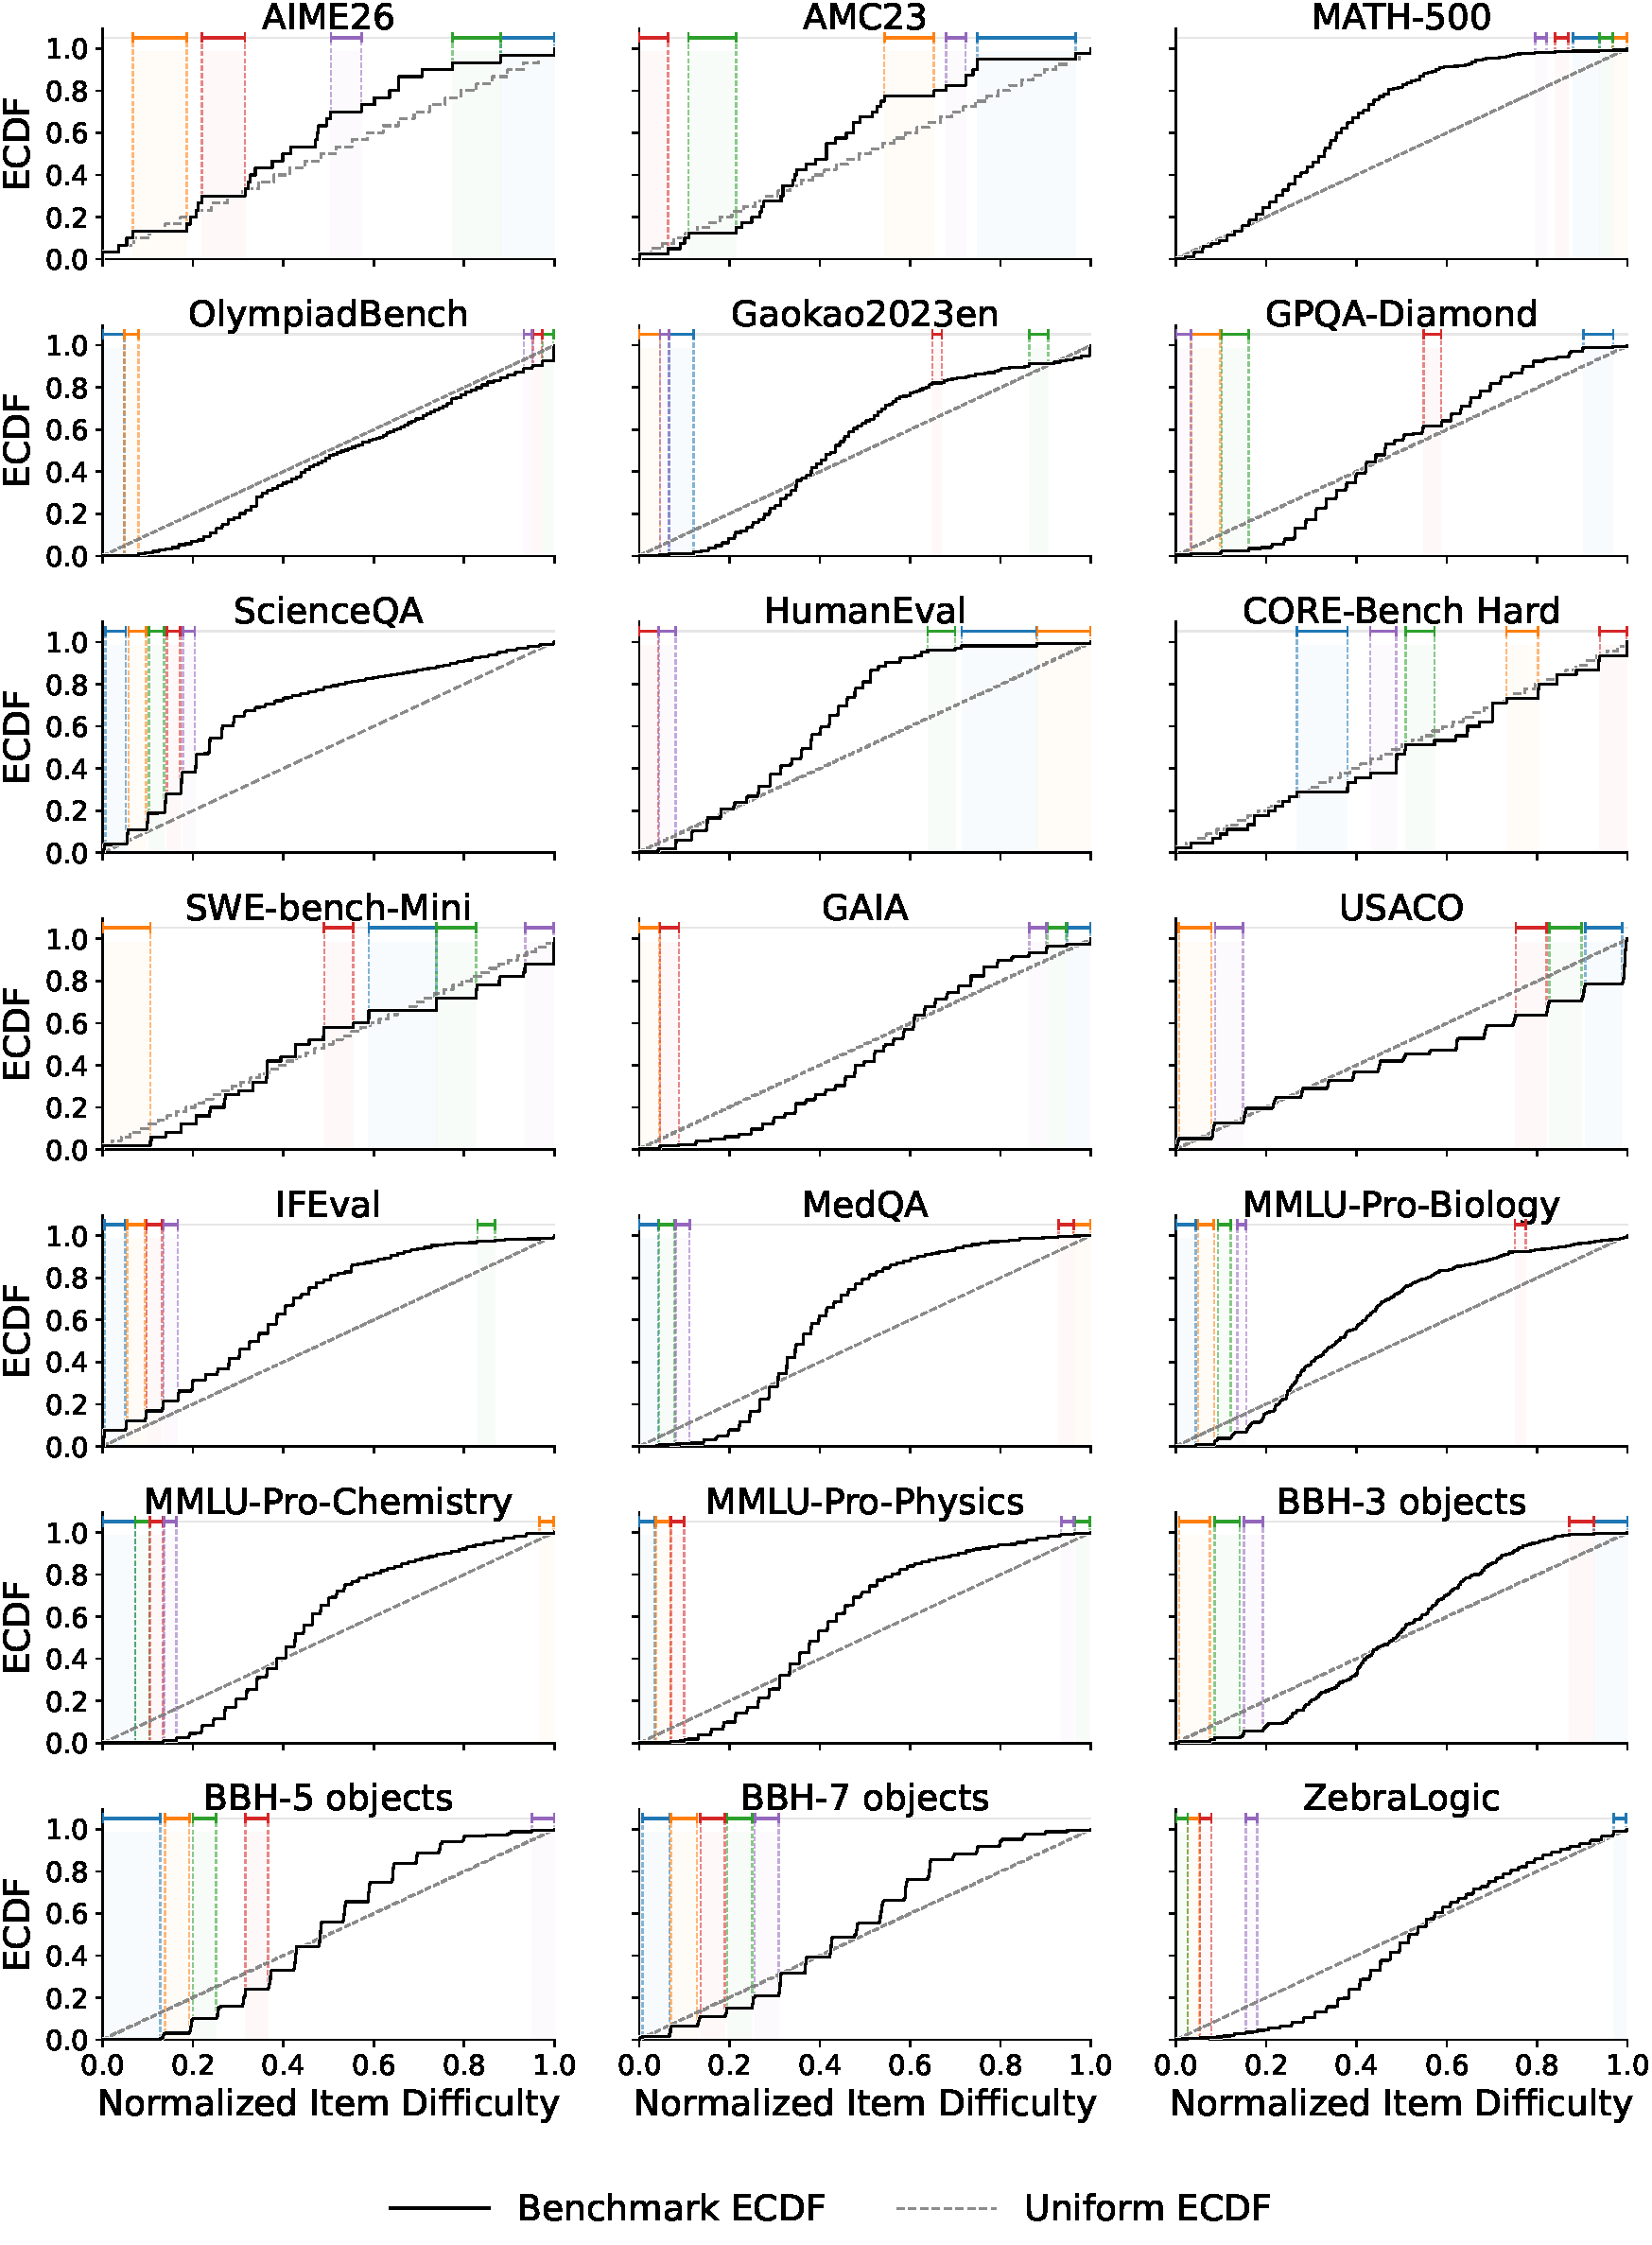
\includegraphics[width=0.95\textwidth,height=0.8\textheight]{Fig/appendix_result.pdf}
    \caption{\textbf{补充的基准难度分布。}
    每个面板展示一个基准归一化题目难度的 ECDF。黑色曲线表示基准 ECDF，灰色虚线表示均匀 ECDF，我们将其用作目标难度分布。偏离均匀 ECDF 表示相对于这一中性目标分布的失配。彩色阴影区间标出排序后题目难度之间五个最大的相邻间隔。}
    \label{fig:appendix_result}
\end{figure*}

\section{基准校准}
\label{sec:app_benchmark_cal}
\paragraph{问题设定。}
测度失配的视角提示了一种重新设计基准的自然方式：调整基准经验测度，使其更好地匹配目标评测分布。考虑基准
\[
B=\{x_1,\ldots,x_n\},
\]
其中每道题 \(x_i\) 具有估计难度 \(z_i\in[0,1]\)。该基准在难度轴上诱导经验测度
\[
\nu_B=\frac{1}{n}\sum_{i=1}^n \delta_{z_i}
\]
。给定目标分布 \(\mu\in\mathcal P([0,1])\)，基准校准旨在构造一个新基准 \(B'\)，使其经验测度 \(\nu_{B'}\) 比 \(\nu_B\) 更接近 \(\mu\)。

在本工作中，我们通过剪枝来实现基准校准。具体而言，我们从原始基准中保留 \(k\) 道题，即选择子集 \(A\subseteq[n]\) 且 \(|A|=k\)。所选题目构成校准后的基准
\[
B_A=\{x_i:i\in A\},
\]
其经验难度测度为
\[
\nu_A=\frac{1}{k}\sum_{i\in A}\delta_{z_i}.
\]
目标是选择 \(A\)，使 \(\nu_A\) 更好地近似目标分布 \(\mu\)，例如以 \(\mathrm{DDM}(B_A;\mu)=W_1(\nu_A,\mu)\) 来衡量。 
% This directly follows the measure-mismatch view: benchmark-induced comparisons are more reliable when the benchmark measure is closer to the intended target measure.

\paragraph{一个简单的校准算法。}
我们使用一个简单的贪心分位数匹配剪枝过程，概括于算法~\ref{alg:benchmark-calibration}。令 \(Q_\mu\) 表示目标分布 \(\mu\) 的分位函数。给定子集大小 \(k\)，我们首先取 \(\mu\) 下 \(k\) 个等概率区间的中点，构造 \(k\) 个目标难度位置：
\[
\tau_t=\frac{t-\frac12}{k},\qquad
q_t=Q_\mu(\tau_t),\qquad t=1,\ldots,k .
\]
然后将这些目标位置匹配到已有基准题。具体而言，在将题目难度归一化到 \([0,1]\) 之后，我们遍历 \(q_1,\ldots,q_k\)，并选择难度最接近当前目标位置的未使用题目：
\[
i_t\in
\arg\min_{i\in [n]\setminus \{i_1,\ldots,i_{t-1}\}}
|z_i-q_t|.
\]
校准子集为 \(A=\{i_1,\ldots,i_k\}\)。

\begin{algorithm}[t]
\caption{分位数匹配的基准校准}
\label{alg:benchmark-calibration}
\begin{algorithmic}[1]
\Require 归一化题目难度 \(z_1,\ldots,z_n\in[0,1]\)，子集大小 \(k\)，目标分位函数 \(Q_\mu\)
\State 初始化已选集合 \(A\leftarrow\emptyset\) 与可用集合 \(U\leftarrow[n]\)
\For{\(t=1,\ldots,k\)}
    \State 设定目标分位水平
    \[
    \tau_t \leftarrow \frac{t-\frac12}{k}
    \]
    \State 设定目标难度位置
    \[
    q_t \leftarrow Q_\mu(\tau_t)
    \]
    \State 选择最接近的未使用题目：
    \[
    i_t \in \arg\min_{i\in U}|z_i-q_t|
    \]
    \State 更新 \(A\leftarrow A\cup\{i_t\}\)
    \State 更新 \(U\leftarrow U\setminus\{i_t\}\)
\EndFor
\State \Return \(A\)
\end{algorithmic}
\end{algorithm}

\subsection{实验设置}

实践中，给定难度轴上的任意目标分布，我们的基准校准想法与算法~\ref{alg:benchmark-calibration} 都可以直接应用。在本实验中，我们研究这种校准能否使单个基准产生的模型排名，与更广泛的同领域基准族更加一致。

我们考虑 \(N=8\) 个数学基准，如表~\ref{tab:benchmark_summary} 所示。对每个基准 \(B_i\)，我们将其视为待校准的源基准，并仅用其余基准 \(\{B_j:j\neq i\}\) 构造模型的外部参照排名。这一留一设计评估：\(B_i\) 的校准版本所诱导的排名，是否与同领域其他基准得到的排名更一致。

具体地，令
\[
B_i=\{x_{i1},\ldots,x_{in_i}\}
\]
为第 \(i\) 个基准，其中题目 \(x_{i\ell}\) 的归一化难度为 \(z_{i\ell}\in[0,1]\)。由于留一参照排名由同领域多个基准汇总而来，它较少受任一源基准特有的难度集中所束缚。因此我们用校准从源基准过度集中的难度区域剪除题目。在没有应用特定目标分布时，我们将校准目标取为均匀分布
\[
\lambda=\mathrm{Unif}[0,1].
\]
这一选择不应被理解为假定留一参照分布恰好是均匀的。相反，均匀校准提供了一种中性的去偏策略：它并不先验地偏袒任何难度区域，并且抵消那些经验质量集中在难度轴狭窄部分的基准。

我们将算法~\ref{alg:benchmark-calibration} 以目标分布 \(\lambda\) 应用于 \(B_i\)，得到大小为 \(k_i\) 的校准子集 \(A_i\subseteq[n_i]\)。校准后的基准为
\[
B_{i,A_i}=\{x_{i\ell}:\ell\in A_i\}.
\]

假设所有基准评估相同的 \(M\) 个模型。令 \(S_i(m)\) 表示模型 \(m\) 在完整源基准 \(B_i\) 上的平均分数，令 \(S_i(A_i,m)\) 表示其在校准子集上的平均分数。未校准排名由
\[
S_i(m),\qquad m=1,\ldots,M,
\]
诱导，而校准排名由
\[
S_i(A_i,m),\qquad m=1,\ldots,M.
\]

对留一参照排名，我们在其余基准上汇总模型分数：
\[
S^{\mathrm{ref}}_{-i}(m)
=
\frac{1}{N-1}\sum_{j\neq i} S_j(m).
\]
由 \(S^{\mathrm{ref}}_{-i}(m)\) 诱导的排名作为源基准 \(B_i\) 的外部参照排名。

对每个源基准，我们计算源诱导排名与留一参照排名之间的 Spearman 与 Kendall 相关，包括校准前与校准后。校准后相关提高，表明把源基准剪枝到更均衡的难度分布，使其模型比较与更广泛的同领域基准族更加一致。

\begin{table*}[t]
\centering
\small
\caption{
\textbf{八个数学基准上的基准校准结果。}
对每个源基准，\textbf{完整}表示原始基准，
\textbf{随机}表示同等规模的 30 个随机剪枝子集的平均，
\textbf{校准}表示我们的分位数匹配基准校准算法产生的校准子集。
Spearman 与 Kendall 衡量与留一参照排名的一致性。
我们报告 \(W_1(\nu,\mathrm{Unif})\) 作为机制指标，以验证校准使所选基准测度更接近中性均匀分布。加粗值表示每个基准、每个指标上 \textbf{完整}、\textbf{随机} 与 \textbf{校准} 中的最佳结果。
}
\label{tab:benchmark_calibration}
\begin{adjustbox}{width=\textwidth}
\begin{tabular}{lccccccccc}
\toprule
& \multicolumn{3}{c}{\textbf{Spearman $\uparrow$}}
& \multicolumn{3}{c}{\textbf{Kendall $\uparrow$}}
& \multicolumn{3}{c}{\(\boldsymbol{W_1(\nu,\mathrm{Unif})}\) \(\boldsymbol{\downarrow}\)} \\
\cmidrule(lr){2-4}
\cmidrule(lr){5-7}
\cmidrule(lr){8-10}
\textbf{基准}
& \textbf{完整} & \textbf{随机} & \textbf{校准}
& \textbf{完整} & \textbf{随机} & \textbf{校准}
& \textbf{完整} & \textbf{随机} & \textbf{校准} \\
\midrule
Minerva-Math  & 0.601 & 0.649 & \textbf{0.790} & 0.455 & 0.514 & \textbf{0.667} & 0.122 & 0.115 & \textbf{0.005} \\
MATH-500      & 0.930 & 0.942 & \textbf{0.958} & 0.879 & 0.878 & \textbf{0.909} & 0.164 & 0.165 & \textbf{0.099} \\
Gaokao2023en  & 0.888 & 0.895 & \textbf{0.951} & 0.788 & 0.790 & \textbf{0.879} & 0.088 & 0.086 & \textbf{0.029} \\
AIME24        & \textbf{0.944} & 0.942 & \textbf{0.944} & \textbf{0.848} & 0.847 & \textbf{0.848} & 0.077 & 0.108 & \textbf{0.019} \\
AIME25        & 0.958 & 0.936 & \textbf{0.972} & 0.909 & 0.854 & \textbf{0.915} & 0.079 & 0.126 & \textbf{0.020} \\
AIME26        & 0.949 & 0.950 & \textbf{0.970} & 0.870 & 0.867 & \textbf{0.901} & 0.085 & 0.108 & \textbf{0.017} \\
AMC23         & \textbf{0.937} & 0.934 & \textbf{0.937} & \textbf{0.848} & \textbf{0.848} & \textbf{0.848} & 0.089 & 0.093 & \textbf{0.025} \\
OlympiadBench & \textbf{0.916} & 0.910 & \textbf{0.916} & \textbf{0.818} & 0.806 & \textbf{0.818} & 0.064 & 0.067 & \textbf{0.008} \\
\midrule
平均       & 0.890 & 0.895 & \textbf{0.930} & 0.802 & 0.801 & \textbf{0.848} & 0.096 & 0.109 & \textbf{0.028} \\
\bottomrule
\end{tabular}
\end{adjustbox}
\end{table*}
\subsection{结果}

实验结果见表~\ref{tab:benchmark_calibration}。结果表明，我们的校准算法提高了源基准排名与留一参照排名之间的一致性。平均而言，校准将 Spearman 相关从 \(0.890\) 提高到 \(0.930\)，将 Kendall 相关从 \(0.802\) 提高到 \(0.848\)。改进在初始一致性较弱的基准上尤其明显。值得注意的是，在 Minerva-Math 上，完整基准与参照排名的 Spearman 与 Kendall 相关分别只有 \(0.601\) 与 \(0.455\)，而校准将其分别提高到 \(0.790\) 与 \(0.667\)。类似地，在 Gaokao2023en 上，校准将 Spearman 从 \(0.888\) 提高到 \(0.951\)，将 Kendall 从 \(0.788\) 提高到 \(0.879\)。对其余基准，初始一致性已经很高，改进空间较小；尽管如此，校准在使用剪枝后基准的同时，始终保持了这一高水平一致性。

我们加入一个随机剪枝基线，其剪枝规模与校准子集相同，并在 30 次随机试验上取平均。随机剪枝不如校准有效：它的平均 Spearman 为 \(0.895\)，平均 Kendall 为 \(0.801\)，都低于校准子集。我们还报告 \(W_1(\nu,\mathrm{Unif})\) 作为机制指标。校准在所有基准上一致地减小该距离，将平均值从 \(0.096\) 降到 \(0.028\)。相反，随机剪枝平均而言并不减小该距离，平均值为 \(0.109\)。这表明改进并非仅仅因为使用了更小的基准，而是来自选择那些经验难度测度更好地匹配中性校准目标的题目。


\section{\textsc{BenchFill} 的补充细节与实验结果}



\newpage
\begin{algorithm}[t]
\caption{\textsc{BenchFill}}
\label{alg:gap_filling}
\begin{algorithmic}[1]
\Require 带归一化难度的基准题 $\{(x_i,z_i)\}_{i=1}^n$；目标间隔 $[z_L,z_R]$；改写 LLM $\mathcal{G}$；有效性评判器 $\mathcal{J}$；IRT 评测 LLM $\{M_j\}_{j=1}^m$ 及其预先估计的 IRT 能力 $\{\hat{\theta}_j\}_{j=1}^m$；每个 LLM 的试验次数 $\{K_j\}_{j=1}^m$；父题数 $R$；每个父题的子题数 $C$；参照列表预算 $L$；最大轮数 $T$；归一化 $[0,1]$ 标尺上的容差 $\tau$。
\Ensure 一道提议的缺口填补题目 $x^\star_{\mathrm{item}}$。

\State 设定目标难度 $z^\star \gets (z_L+z_R)/2$。
\State 用所选间隔附近已有的标注题目--难度对初始化记忆 $\mathcal{M}$。
\State 初始化有效候选集 $\mathcal{C}_{\mathrm{valid}} \gets \emptyset$。

\For{$t=1,\dots,T$}
    \State 检索父题集 $\mathcal{S}_t \subseteq \mathcal{M}$，其中至多 $R$ 道题，其标注难度最接近 $z^\star$。
    \State 用 $z^\star$ 附近的题目--难度对构造参照列表 $\mathcal{R}_t \subseteq \mathcal{M}$，满足 $|\mathcal{R}_t|\le L$；在可得时，至多一半取自低于 $z^\star$ 的题目，其余取自高于 $z^\star$ 的题目。
    
    \For{每个父题 $(x_p,z_p) \in \mathcal{S}_t$}
        \State 为了提示，将 $z^\star$ 与 $\mathcal{R}_t$ 中显示的难度从 $[0,1]$ 重新缩放到 $[0,10]$。
        \State 以父题、目标难度和参照列表为条件，将父题改写为 $C$ 个子题：
        \[
        \{x_{p,1},\dots,x_{p,C}\}
        \gets
        \mathcal{G}(x_p, z^\star, \mathcal{R}_t).
        \]
        
        \For{每个子题 $x_{p,c}$}
            \If{$\mathcal{J}$ 核验 $x_{p,c}$ 的参考答案正确}
                \For{$j=1,\dots,m$}
                    \State 用 LLM $M_j$ 在 $x_{p,c}$ 上做 $K_j$ 次试验，并记录 $c_j$ 次正确回答。
                \EndFor
                \State 通过在线校准估计题目难度：
                \[
                \hat{b}_{p,c}
                \gets
                \arg\max_b
                \sum_{j=1}^{m}
                \left[
                c_j\log \sigma(\hat{\theta}_j-b)
                +
                (K_j-c_j)\log\bigl(1-\sigma(\hat{\theta}_j-b)\bigr)
                \right].
                \]
                \State 用与原始基准相同的变换归一化 $\hat{b}_{p,c}$，得到 $\hat{z}_{p,c}$。
                \State 将 $(x_{p,c},\hat{z}_{p,c})$ 加入 $\mathcal{M}$。
                \State 将 $(x_{p,c},\hat{z}_{p,c})$ 加入 $\mathcal{C}_{\mathrm{valid}}$。
            \EndIf
        \EndFor
    \EndFor
    
    \If{$\mathcal{C}_{\mathrm{valid}} \neq \emptyset$ and
    $\min_{(x,\hat{z})\in \mathcal{C}_{\mathrm{valid}}} |\hat{z}-z^\star| \le \tau$}
        \State \textbf{跳出}
    \EndIf
\EndFor

\If{$\mathcal{C}_{\mathrm{valid}} = \emptyset$}
    \State \Return 失败
\EndIf

\State 选择最接近的有效子题：
\[
(x^\star_{\mathrm{item}},\hat{z}^\star)
\gets
\arg\min_{(x,\hat{z})\in \mathcal{C}_{\mathrm{valid}}}
|\hat{z}-z^\star|.
\]
\State \Return $x^\star_{\mathrm{item}}$ 作为提议的缺口填补题目，并交由人类专家审核。
\end{algorithmic}
\end{algorithm}

\subsection{实现细节}
\label{sec:app_gap}


对每个基准，我们关注其估计难度分布中三个最显著的间隔，并为每个间隔改写一道题。由于当提示中给出目标难度时，LLM 可能无法可靠区分归一化 $[0,1]$ 难度标尺上的细小数值差异，我们在提示时将难度值重新缩放到 $[0,10]$，而所有报告的指标仍保持在原始归一化标尺上。

对参照列表，我们在目标难度两侧都纳入附近的题目--难度对。具体而言，一半参照题选自难度低于目标且最接近目标的题目，另一半选自难度高于目标且最接近目标的题目。这为改写器提供了期望难度水平附近的局部双向上下文。完整的改写提示模板如下。

对难度标注，我们使用与原始难度估计阶段相同的 LLM 集合和相同的生成配置。若迄今找到的最佳有效题目在归一化 $[0,1]$ 标尺上与目标难度的距离处于容差 $\tau=0.01$ 之内，搜索提前停止；否则在达到最大轮数后停止。然后我们选择标注难度最接近目标的有效题目。在插入基准之前，每道入选题目都由至少三位人类专家进行人工有效性检查，以核验其正确性。

我们额外实现了一个预算匹配的 best-of-\(N\) 均匀父题改写基线。对每个目标间隔 \(g\)，令 \(T_g\) 表示 \textsc{BenchFill} 在停止前实际运行的轮数。由于 \textsc{BenchFill} 每轮改写 \(4\) 个父题、每个父题产生 \(4\) 个子题，该间隔的提议预算为 \(T_g \times 4 \times 4 = 16T_g\) 个子题。为匹配这一预算，基线均匀抽取 \(4\) 道已有基准题作为父题，并让同一个改写 LLM 以父题和目标难度为条件，从每个父题改写出 \(4T_g\) 个子题。难度标注之后，它在所有生成候选中选择难度最接近目标的有效子题。因此，基线使用与 \textsc{BenchFill} 相同的总改写预算和相同的最终选择规则，但不使用难度感知的父题检索、附近参照列表或迭代记忆更新。

\begin{center}
\begin{tcolorbox}[
    title={改写器提示模板},
    label={box:proposer_prompt},
    width=\linewidth,
    colback=white,
    colframe=black,
    boxrule=0.5pt,
    left=6pt,
    right=6pt,
    top=6pt,
    bottom=6pt,
    fonttitle=\bfseries,
    fontupper=\ttfamily\small,
]

将下面的父题改写为\textbf{恰好 1} 道新的基准题变体。
目标难度（0--10 标尺，越高越难）：
\textbf{\{target\_difficulty\}}。

\medskip
\textbf{父题}（将此题改写为新变体——不要复制其具体措辞、数字或答案）：

\{parent.question\}

答案：\{parent.reference\_answer\}

难度（0--10）：\{parent.difficulty\} $|$ delta \{target - parent.difficulty\} $|$ generate \texttt{\{harder|easier\}}

\medskip
\textbf{记忆题目}（仅用作风格/难度参照，不要复制）：

\medskip
--- 记忆 1 ---

\{memory[0].question\}

答案：\{memory[0].reference\_answer\}

难度（0--10）：\{memory[0].difficulty\} $|$ delta \{target - memory[0].difficulty\} $|$ generate \texttt{\{harder|easier\}}

\medskip
--- 记忆 2 ---

\{memory[1].question\}

答案：\{memory[1].reference\_answer\}

难度（0--10）：\{memory[1].difficulty\} $|$ delta \{target - memory[1].difficulty\} $|$ generate \texttt{\{harder|easier\}}

\medskip
...（每个记忆题目一块）...

\medskip
\textbf{只}返回一个 markdown 代码块：第一行以 \texttt{\textasciigrave\textasciigrave\textasciigrave{}json} 开始，然后换行，然后是一个\textbf{恰好含 1} 个元素的 JSON 数组，再单独一行以 \texttt{\textasciigrave\textasciigrave\textasciigrave} 结束。结束围栏之后不要放任何内容。

\medskip
在 JSON \textbf{语法完整}之前不要停止：每个字符串值都以 \texttt{"} 闭合，每个对象都以 \texttt{\}} 闭合，数组以 \texttt{]} 结束，然后是结束用的 \texttt{\textasciigrave\textasciigrave\textasciigrave} 行。

\medskip
该数组必须\textbf{恰好含 1} 个元素——一个对象，且恰好包含这些键：
\texttt{"id"}（字符串），\texttt{"question"}（字符串），\texttt{"answer"}（字符串）。

\end{tcolorbox}
\end{center}

\subsection{补充实验结果}

% \naicheng{human validation; Does the rewriter perceive difficulty?}

% \jiawen{Empirical Validation beyond gap reduction}

\paragraph{人工验证。}
我们用两阶段验证过程确保生成的缺口填补题目可靠。GPT-5.4 首先作为自动有效性评判器，检查每个候选是否格式良好、其参考答案是否正确；未通过该检查的候选被丢弃并重新生成。人类专家随后独立审核最终入选的题目。在 24 个目标间隔中，有一个最初提议的候选因参考答案错误而未通过 GPT-5.4 检查，并被重新生成。全部 24 道最终入选题目都通过了 GPT-5.4 有效性检查，并随后未经修改或替换地通过了人工审核。

\paragraph{改写器能否感知难度？} 一个自然的问题是，我们的改写器是否确实感知难度，而不是盲目地命中目标难度。我们从两个互补角度考察这一问题：改写器在迭代反馈之前是否已经表现出难度敏感性，以及随后的搜索并标注循环是否进一步提高与目标难度的对齐。

首先，为了把改写器自身的难度感知与后来的 IRT 反馈及迭代搜索隔离开，我们只分析每个缺口填补情形的第一轮生成。在此阶段，改写器以指定的目标难度为条件，但尚未收到其生成子题的标注难度反馈。图~\ref{fig:first_round_calibration} 展示了全部 8 个基准、每个基准 3 个目标间隔上，指定目标难度与有效首轮子题的标注难度。在大多数基准内，更高的指定目标产生更高的平均标注难度，并且分隔良好的目标通常诱导出不同的子题难度分布。这表明，在引入迭代反馈之前，改写器对指定难度标尺已经具有非平凡的敏感性。

其次，我们考察搜索并标注循环是否进一步提高目标对齐。图~\ref{fig:multi_round_deviation} 展示了每个基准中一个有代表性的缺口填补情形。在这些情形中，平均绝对目标偏差总体上从第一轮下降到最后一轮，并且在大多数情形中生成的子题也更集中于目标附近。这表明，迭代循环利用 IRT 标注与更新后的记忆，进一步细化了改写器最初的难度信号。

\begin{figure*}[t]
    \centering
    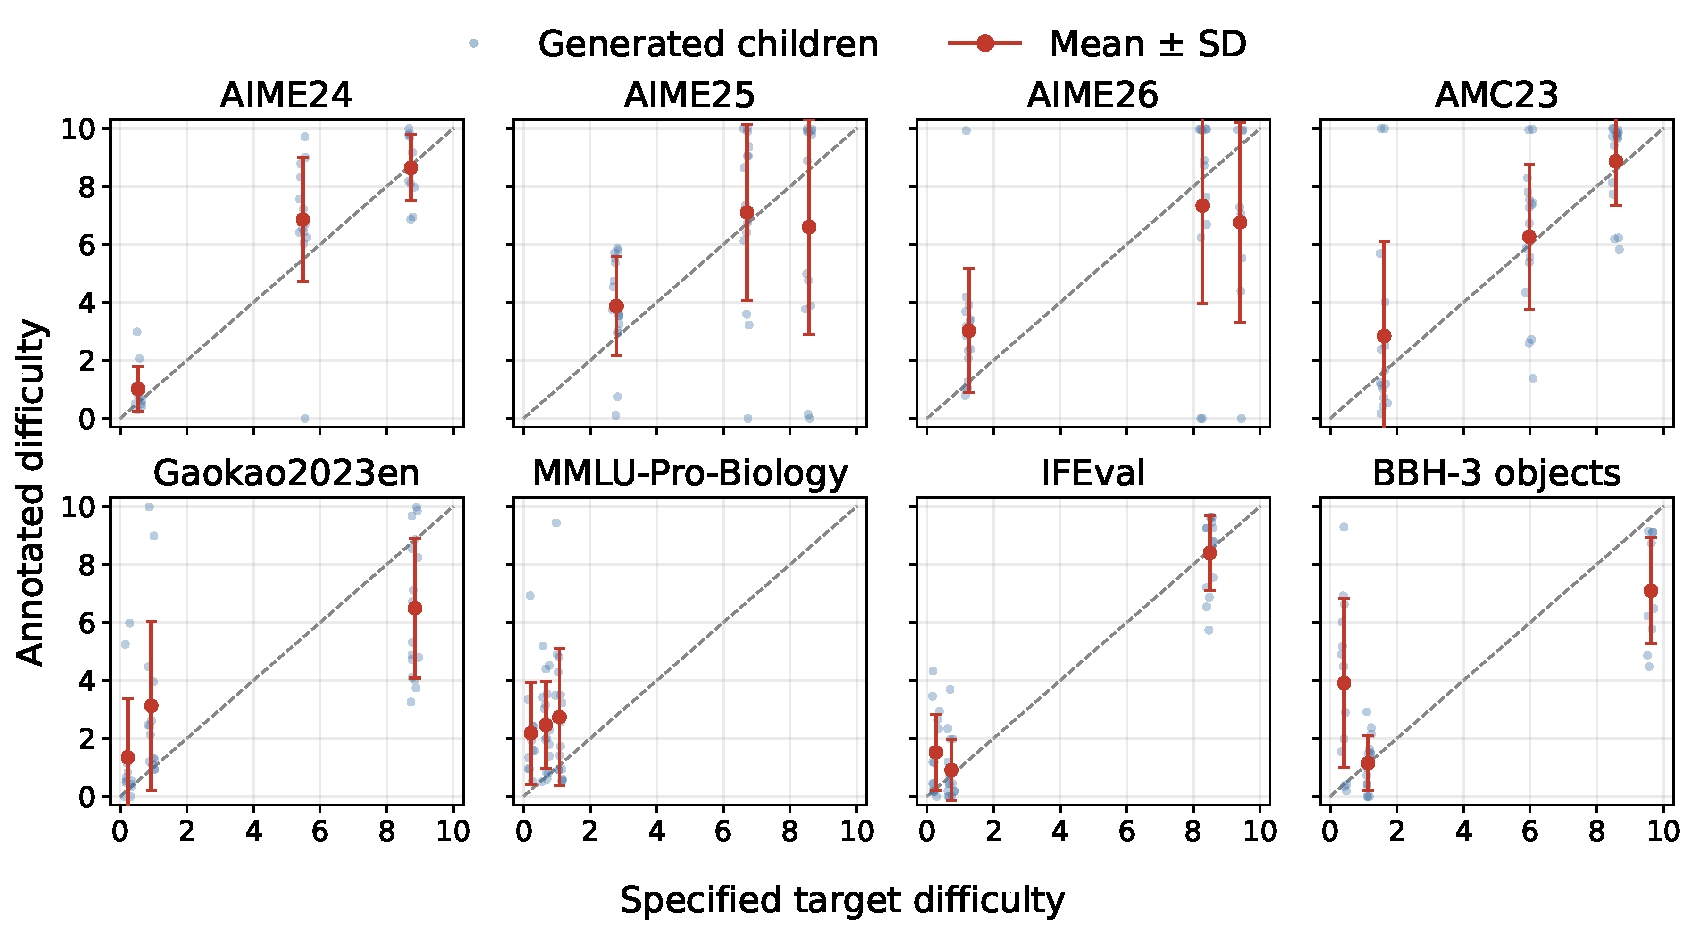
\includegraphics[width=\textwidth]{Fig/first_round_calibration.pdf}
    \caption{\textbf{指定目标难度与标注难度的首轮对齐。}
    每个面板对应一个基准。横轴为指定目标难度，纵轴为有效首轮子题的标注难度。蓝点表示单个生成子题，红色标记表示每个目标难度的均值与标准差。虚线对角线表示完全对齐。为便于阅读，两个坐标轴都显示在 0--10 标尺上，对应于 $[0,1]$ 中的归一化难度乘以 10。在大多数基准内，更高的指定目标在第一轮、即纳入任何迭代反馈之前，就已经产生更高的标注难度。}
    \label{fig:first_round_calibration}
\end{figure*}


\begin{figure*}[t]
    \centering
    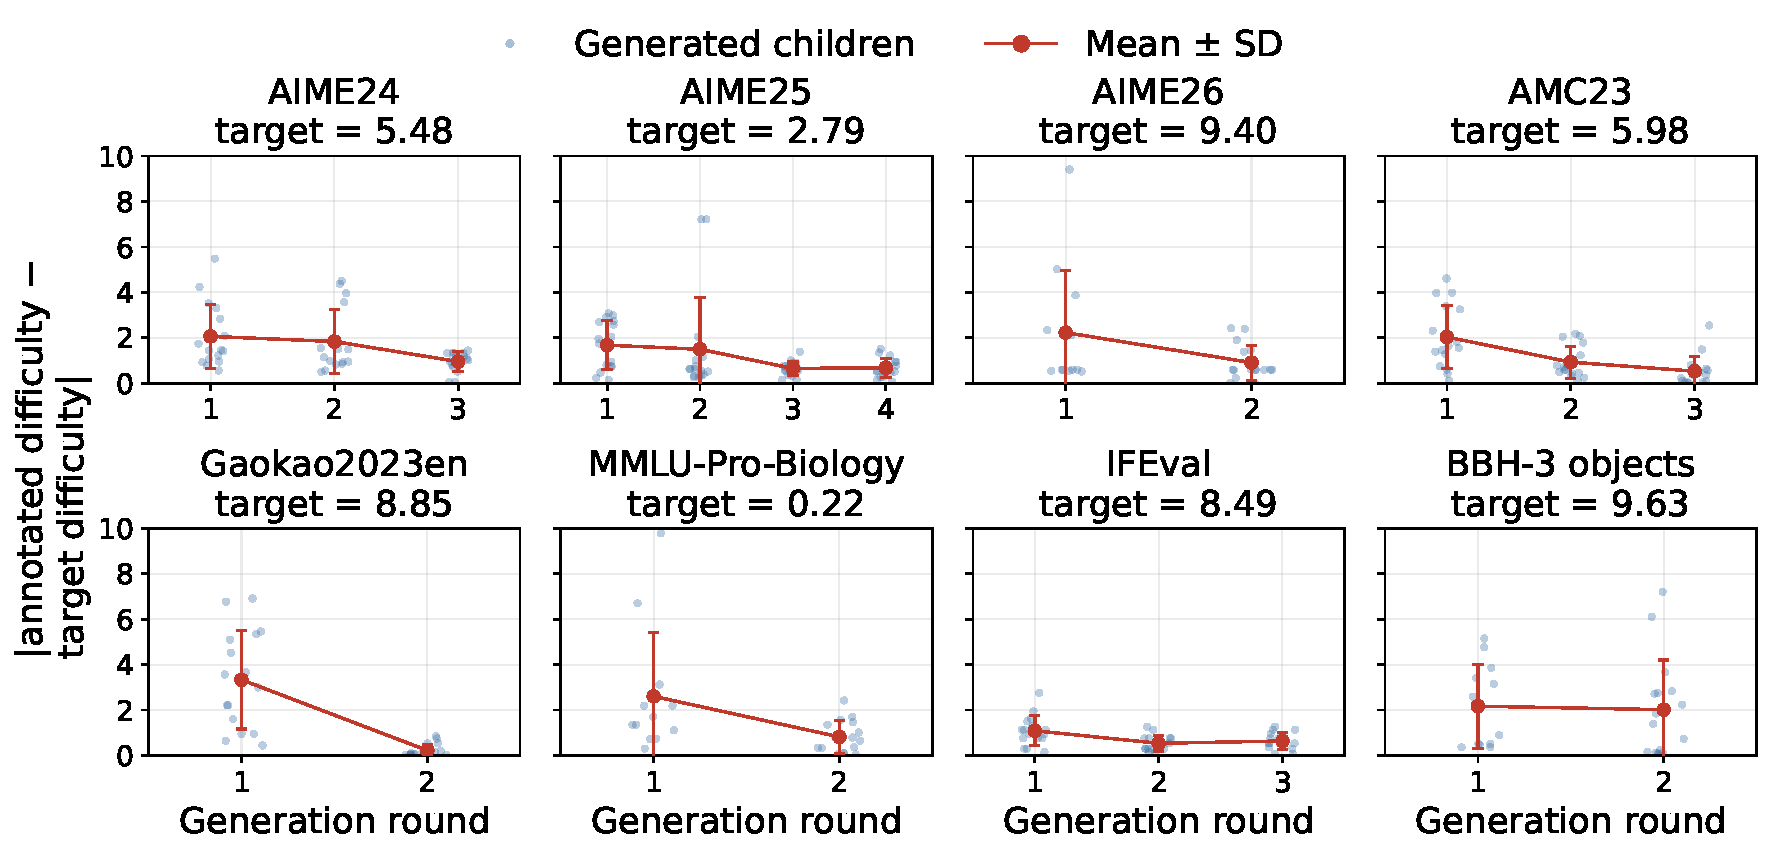
\includegraphics[width=\textwidth]{Fig/multiround_target_deviation.pdf}
    \caption{\textbf{\textsc{BenchFill} 搜索过程中的多轮目标对齐。}
    每个面板展示来自不同基准的一个有代表性的缺口填补情形。横轴为生成轮次，纵轴为生成子题的绝对目标偏差 $|\hat{z} - z^\star|$。为便于阅读，目标难度与绝对偏差都乘以 10。蓝点表示单个生成子题，红色标记表示该轮的均值与标准差。
    在大多数情形中，平均目标偏差随轮次下降，生成的子题更集中于目标附近，表明搜索并标注循环在改写器最初的难度敏感性之外进一步提高了目标对齐。}
    \label{fig:multi_round_deviation}
\end{figure*}


\paragraph{检测局部模型改进。}
我们进一步考察 \textsc{BenchFill} 是否在缩小难度间隔之外，提高基准检测局部模型改进的能力。我们在 AIME24、AIME25 与 AIME26 中各考虑一个目标间隔，并比较三种基准变体：\texttt{原始}、\texttt{原始 + BenchFill} 与 \texttt{原始 + 基线}。两种扩充方法都向原始基准恰好插入一道题。我们进行轻度 SFT，使模型在目标间隔区域附近得到改进。每道题在 SFT 前后各用 32 次 rollout 评估，并用单侧分层随机化检验（$p<0.05$）检验增益是否在统计上可检测。

如表~\ref{tab:localized_detection} 所示，\texttt{原始 + BenchFill} 在全部三个情形中都检测到 SFT 后的正增益（3/3），而 \texttt{原始} 与 \texttt{原始 + 基线} 都没有检测到（各为 0/3）。这表明 \textsc{BenchFill} 并非仅仅改进它所优化的指标；通过填补覆盖不足的难度区域，它使基准对否则会被遗漏的局部模型改进更加敏感。



\begin{table*}[t]
\centering
\caption{\textbf{局部改进检测结果。}
每种扩充方法都向原始的 30 题基准增加一道题。
增益表示平均准确率的变化。
单侧分层随机化检验在每道题内，用 100{,}000 次置换将 rollout 结果在 SFT 前与 SFT 后条件之间随机重新分配。
加粗表示在 $p<0.05$ 下检测到正增益的变体。}
\label{tab:localized_detection}
\small
\setlength{\tabcolsep}{5pt}
\begin{tabular}{llccc}
\toprule
\textbf{情形}
& \textbf{基准变体}
& \textbf{增益}
& \textbf{单侧 $p$}
& \textbf{是否检出} \\
\midrule
\multirow{3}{*}{\shortstack[l]{AIME24\\Olmo-3.1-32B-Think}}
& \texttt{原始}
& +0.104 & 0.500100 & $\times$ \\
& \textbf{\texttt{原始 + BenchFill}}
& \textbf{+2.419} & \textbf{0.005940} & $\checkmark$ \\
& \texttt{原始 + 基线}
& +0.202 & 0.458000 & $\times$ \\
\midrule
\multirow{3}{*}{\shortstack[l]{AIME25\\Phi-4}}
& \texttt{原始}
& +1.042 & 0.184100 & $\times$ \\
& \textbf{\texttt{原始 + BenchFill}}
& \textbf{+3.730} & \textbf{0.000450} & $\checkmark$ \\
& \texttt{原始 + 基线}
& +0.907 & 0.214200 & $\times$ \\
\midrule
\multirow{3}{*}{\shortstack[l]{AIME26\\Llama-3.1-8B-Instruct}}
& \texttt{原始}
& +0.208 & 0.418400 & $\times$ \\
& \textbf{\texttt{原始 + BenchFill}}
& \textbf{+3.427} & \textbf{0.000010} & $\checkmark$ \\
& \texttt{原始 + 基线}
& +0.101 & 0.498000 & $\times$ \\
\bottomrule
\end{tabular}
\end{table*}

\paragraph{代表性示例。}
为定性展示生成的缺口填补题目，我们在表~\ref{tab:gap_filling_examples} 中给出有代表性的改写示例。每个示例同时给出最终入选题目及其在基准中的原始祖先，以及祖先难度、目标难度和入选题目的标注难度。这些示例说明 \textsc{BenchFill} 如何修改已有基准题，以到达先前覆盖不足的难度水平。



% To illustrate how \textsc{BenchFill} approaches the target difficulty over multiple rounds, we provide several example search trajectories in Fig.~\ref{fig:gap_filling_examples}. Each subplot corresponds to one benchmark--gap pair. These examples provide a qualitative view of how the rewrite-and-annotate search progressively moves toward the target difficulty. We also provide representative rewriting examples in Tab.~\ref{tab:gap_filling_examples}, showing each final selected item together with its original ancestor item from the benchmark, as well as the target difficulty and annotated difficulty of the selected item.


% \begin{figure*}[t]
%     \centering
%     \includegraphics[width=\textwidth]{Fig/gap_example.pdf}
%     \caption{\textbf{Example \textsc{BenchFill} search trajectories.}
%     Each panel shows one gap-filling example for a specific benchmark--gap pair.
%     The horizontal axis denotes the search round, and the vertical axis denotes the absolute deviation between the best valid item found up to round $t$ and the target difficulty,
%     $\left|\hat{z}_{\mathrm{best}}^{(t)} - z^\star\right|$.
%     Values closer to zero indicate better alignment with the target difficulty.
%     The tolerance band is set to $0.01$, and the search terminates once the best valid item falls within this band.
%     The decreasing trajectories show that \textsc{BenchFill} progressively finds valid items closer to the target difficulty.}
%     \label{fig:gap_filling_examples}
% \end{figure*}

% \begin{table*}[t]
% \centering
% \footnotesize
% \setlength{\tabcolsep}{2.5pt}
% \renewcommand{\arraystretch}{1.15}
% \caption{
% \textbf{Representative pairs of original benchmark ancestors and final selected items produced by \textsc{BenchFill}.}
% All difficulty values are normalized to $[0,1]$.
% The main change from the ancestor item to the selected item is highlighted. For selected items, values in parentheses denote the target difficulty.
% }
% \label{tab:gap_filling_examples}
% \begin{tabularx}{\textwidth}{
% >{\centering\arraybackslash}p{0.125\textwidth}
% >{\hspace{3pt}\raggedright\arraybackslash}p{0.275\textwidth}
% >{\centering\arraybackslash}p{0.070\textwidth}
% >{\raggedright\arraybackslash}p{0.395\textwidth}
% >{\centering\arraybackslash}p{0.090\textwidth}
% }
% \toprule
% \textbf{Benchmark}
% & \multicolumn{2}{c}{\textbf{Original benchmark ancestor}}
% & \multicolumn{2}{c}{\textbf{Selected gap-filling item}} \\
% \cmidrule(lr){2-3}
% \cmidrule(lr){4-5}
% & \multicolumn{1}{c}{\textbf{Item}}
% & \textbf{Diff.}
% & \multicolumn{1}{c}{\textbf{Item}}
% & \shortstack{\textbf{Diff.}} \\
% \midrule

% \textbf{AMC23}
% &
% For how many ordered pairs $(a,b)$ of integers does the polynomial $x^3+ax^2+bx+\colorbox{red!20}{6}$ have $3$ distinct integer roots?
% &
% $0.749$
% &
% Find the number of ordered pairs $(a,b)$ of integers such that the polynomial $x^3+ax^2+bx+\colorbox{red!20}{60}$ has exactly three distinct integer roots.
% &
% $0.859$ $(0.857)$
% \\

% \midrule

% \textbf{Gaokao2023en}
% & On an \colorbox{red!20}{$8 \times 8$ chessboard,} \colorbox{red!20}{6 black rooks} and $k$ white rooks are placed on different cells so that each rook only attacks rooks of the opposite color. Compute the maximum possible value of $k$. Two rooks attack each other if they are in the same row or column and no rooks are between them.
% &
% $0.864$
% & On a \colorbox{red!20}{$10 \times 10$ toroidal chessboard}, where the first and last rows are adjacent and the first and last columns are adjacent, \colorbox{red!20}{7 black rooks} and $k$ white rooks are placed on distinct squares such that no rook attacks another rook of the same color. A rook attacks another if they share a row or column with no intervening rooks; on this board, this condition applies in both directions along the row or column. Determine the maximum possible value of $k$.
% &
% $0.882$ $(0.885)$
% \\

% \midrule

% \textbf{AIME25}
% &
% The $27$ cells of a $3 \times 9$ grid are filled with the numbers $1$ through $9$ so that each row contains $9$ different numbers and each $3 \times 3$ block contains $9$ different numbers, as in the first three rows of a Sudoku puzzle. The number of different ways to fill \colorbox{red!20}{such a grid} can be written as $p^a q^b r^c s^d$, where $p,q,r,s$ are distinct primes and $a,b,c,d$ are positive integers. Find $pa+qb+rc+sd$.
% &
% $0.592$
% &
% The $27$ cells of a $3 \times 9$ grid are filled with the numbers $1$ through $9$ so that each row contains $9$ different numbers and each $3 \times 3$ block contains $9$ different numbers, as in the first three rows of a Sudoku puzzle. The number of different ways to fill such a grid \colorbox{red!20}{such that the first column contains the} \colorbox{red!20}{numbers $1,2,3$} in that order can be written as $p^a q^b r^c s^d$, where $p,q,r,s$ are distinct primes and $a,b,c,d$ are positive integers. Find $pa+qb+rc+sd$.
% &
% $0.675$ $(0.671)$
% \\

% \bottomrule
% \end{tabularx}
% \end{table*}

\begin{table*}[t]
\centering
\footnotesize
\setlength{\tabcolsep}{2.5pt}
\renewcommand{\arraystretch}{1.15}
\caption{
\textbf{\textsc{BenchFill} 产生的原始基准祖先与最终入选题目的代表性配对。}
所有难度值都归一化到 $[0,1]$。
从祖先题目到入选题目的主要改动被高亮。对入选题目，括号中的值表示目标难度。
}
\label{tab:gap_filling_examples}
\begin{tabularx}{\textwidth}{
>{\centering\arraybackslash}p{0.125\textwidth}
>{\hspace{3pt}\raggedright\arraybackslash}p{0.275\textwidth}
>{\centering\arraybackslash}p{0.070\textwidth}
>{\raggedright\arraybackslash}p{0.395\textwidth}
>{\centering\arraybackslash}p{0.090\textwidth}
}
\toprule
\textbf{基准}
& \multicolumn{2}{c}{\textbf{原始基准祖先}}
& \multicolumn{2}{c}{\textbf{入选的缺口填补题目}} \\
\cmidrule(lr){2-3}
\cmidrule(lr){4-5}
& \multicolumn{1}{c}{\textbf{题目}}
& \textbf{难度}
& \multicolumn{1}{c}{\textbf{题目}}
& \shortstack{\textbf{难度}} \\
\midrule

\textbf{AMC23}
&
对多少个整数 $n$，表达式 $\sqrt{\frac{\log (n^2) - (\log n)^2}{\log n - \colorbox{red!20}{3}}}$ 表示一个实数，其中 $\log$ 表示以 $10$ 为底的对数？
&
$0.535$
&
求使得 $\sqrt{\frac{\log (n^2) - (\log n)^2}{\log n - \colorbox{red!20}{1}}}$ 表示实数的整数 $n$ 的个数，其中 $\log$ 表示以 $10$ 为底的对数。
&
$0.597$ $(0.598)$
\\

\midrule

\textbf{Gaokao2023en}
& 在一个\colorbox{red!20}{$8 \times 8$ 的棋盘上}放置\colorbox{red!20}{$6$ 枚黑车}和 $k$ 枚白车，且它们位于不同格子，使得每枚车只攻击相反颜色的车。求 $k$ 的最大可能值。（若两枚车位于同一行或同一列且中间没有其他车，则它们互相攻击。）
&
$0.864$
& 在一个\colorbox{red!20}{$9 \times 9$ 的棋盘上}放置\colorbox{red!20}{$7$ 枚黑车}和 $k$ 枚白车，且它们位于不同格子，使得每枚车只攻击相反颜色的车。$k$ 的最大可能值是多少？（若两枚车位于同一行或同一列且中间没有其他车，则它们互相攻击。）
&
$0.886$ $(0.885)$
\\

\midrule

\textbf{AIME25}
&
Alex 用两条在圆盘中心相交的垂直直径，将圆盘分成\colorbox{red!20}{四个象限}。他再画\colorbox{red!20}{$25$ 条线段}穿过圆盘，每条线段随机连接圆周上\colorbox{red!20}{不同象限}中的两点。求这些\colorbox{red!20}{$27$ 条线段}将圆盘分成的区域数的期望。
&
$0.750$
&
圆上画有一条直径，将其分成\colorbox{red!20}{两个半圆区域}。然后画\colorbox{red!20}{$8$ 条弦}，每条弦连接\colorbox{red!20}{一个半圆}边界上的随机点与\colorbox{red!20}{另一个半圆}边界上的随机点。假设所有点独立均匀选取，圆的内部被分成的区域数的期望是多少？
&
$0.674$ $(0.671)$
\\

\bottomrule
\end{tabularx}
\end{table*}



%%%%%%%%%%%%%%%%%%%%%%%%%%%%%%%%%%%%%%%%%%%%%%%%%%%%%%%%%%%%

\newpage
% \FloatBarrier
% \section*{NeurIPS Paper Checklist}

% %%% BEGIN INSTRUCTIONS %%%
% % The checklist is designed to encourage best practices for responsible machine learning research, addressing issues of reproducibility, transparency, research ethics, and societal impact. Do not remove the checklist: {\bf The papers not including the checklist will be desk rejected.} The checklist should follow the references and follow the (optional) supplemental material.  The checklist does NOT count towards the page
% % limit. 

% % Please read the checklist guidelines carefully for information on how to answer these questions. For each question in the checklist:
% % \begin{itemize}
% %     \item You should answer \answerYes{}, \answerNo{}, or \answerNA{}.
% %     \item \answerNA{} means either that the question is Not Applicable for that particular paper or the relevant information is Not Available.
% %     \item Please provide a short (1--2 sentence) justification right after your answer (even for \answerNA). 
% %    % \item {\bf The papers not including the checklist will be desk rejected.}
% % \end{itemize}

% % {\bf The checklist answers are an integral part of your paper submission.} They are visible to the reviewers, area chairs, senior area chairs, and ethics reviewers. You will also be asked to include it (after eventual revisions) with the final version of your paper, and its final version will be published with the paper.

% % The reviewers of your paper will be asked to use the checklist as one of the factors in their evaluation. While \answerYes{} is generally preferable to \answerNo{}, it is perfectly acceptable to answer \answerNo{} provided a proper justification is given (e.g., error bars are not reported because it would be too computationally expensive'' or ``we were unable to find the license for the dataset we used''). In general, answering \answerNo{} or \answerNA{} is not grounds for rejection. While the questions are phrased in a binary way, we acknowledge that the true answer is often more nuanced, so please just use your best judgment and write a justification to elaborate. All supporting evidence can appear either in the main paper or the supplemental material, provided in appendix. If you answer \answerYes{} to a question, in the justification please point to the section(s) where related material for the question can be found.

% % IMPORTANT, please:
% % \begin{itemize}
% %     \item {\bf Delete this instruction block, but keep the section heading ``NeurIPS Paper Checklist"},
% %     \item  {\bf Keep the checklist subsection headings, questions/answers and guidelines below.}
% %     \item {\bf Do not modify the questions and only use the provided macros for your answers}.
% % \end{itemize} 
 

% %%% END INSTRUCTIONS %%%


% \begin{enumerate}

% \item {\bf Claims}
%     \item[] Question: Do the main claims made in the abstract and introduction accurately reflect the paper's contributions and scope?
%     \item[] Answer: \answerYes{} % Replace by \answerYes{}, \answerNo{}, or \answerNA{}.
%     \item[] Justification: The abstract and introduction accurately reflect the contributions and scope of the paper.
%     \item[] Guidelines:
%     \begin{itemize}
%         \item The answer \answerNA{} means that the abstract and introduction do not include the claims made in the paper.
%         \item The abstract and/or introduction should clearly state the claims made, including the contributions made in the paper and important assumptions and limitations. A \answerNo{} or \answerNA{} answer to this question will not be perceived well by the reviewers. 
%         \item The claims made should match theoretical and experimental results, and reflect how much the results can be expected to generalize to other settings. 
%         \item It is fine to include aspirational goals as motivation as long as it is clear that these goals are not attained by the paper. 
%     \end{itemize}

% \item {\bf Limitations}
%     \item[] Question: Does the paper discuss the limitations of the work performed by the authors?
%     \item[] Answer: \answerYes{} % Replace by \answerYes{}, \answerNo{}, or \answerNA{}.
%     \item[] Justification: The limitations are discussed in App.~\ref{sec:app_limitation}.
%     \item[] Guidelines:
%     \begin{itemize}
%         \item The answer \answerNA{} means that the paper has no limitation while the answer \answerNo{} means that the paper has limitations, but those are not discussed in the paper. 
%         \item The authors are encouraged to create a separate ``Limitations'' section in their paper.
%         \item The paper should point out any strong assumptions and how robust the results are to violations of these assumptions (e.g., independence assumptions, noiseless settings, model well-specification, asymptotic approximations only holding locally). The authors should reflect on how these assumptions might be violated in practice and what the implications would be.
%         \item The authors should reflect on the scope of the claims made, e.g., if the approach was only tested on a few datasets or with a few runs. In general, empirical results often depend on implicit assumptions, which should be articulated.
%         \item The authors should reflect on the factors that influence the performance of the approach. For example, a facial recognition algorithm may perform poorly when image resolution is low or images are taken in low lighting. Or a speech-to-text system might not be used reliably to provide closed captions for online lectures because it fails to handle technical jargon.
%         \item The authors should discuss the computational efficiency of the proposed algorithms and how they scale with dataset size.
%         \item If applicable, the authors should discuss possible limitations of their approach to address problems of privacy and fairness.
%         \item While the authors might fear that complete honesty about limitations might be used by reviewers as grounds for rejection, a worse outcome might be that reviewers discover limitations that aren't acknowledged in the paper. The authors should use their best judgment and recognize that individual actions in favor of transparency play an important role in developing norms that preserve the integrity of the community. Reviewers will be specifically instructed to not penalize honesty concerning limitations.
%     \end{itemize}

% \item {\bf Theory assumptions and proofs}
%     \item[] Question: For each theoretical result, does the paper provide the full set of assumptions and a complete (and correct) proof?
%     \item[] Answer: \answerYes{} % Replace by \answerYes{}, \answerNo{}, or \answerNA{}.
%     \item[] Justification: All theoretical results state their assumptions, and complete proofs are provided in App.~\ref{sec:app_proof}.
%     \item[] Guidelines:
%     \begin{itemize}
%         \item The answer \answerNA{} means that the paper does not include theoretical results. 
%         \item All the theorems, formulas, and proofs in the paper should be numbered and cross-referenced.
%         \item All assumptions should be clearly stated or referenced in the statement of any theorems.
%         \item The proofs can either appear in the main paper or the supplemental material, but if they appear in the supplemental material, the authors are encouraged to provide a short proof sketch to provide intuition. 
%         \item Inversely, any informal proof provided in the core of the paper should be complemented by formal proofs provided in appendix or supplemental material.
%         \item Theorems and Lemmas that the proof relies upon should be properly referenced. 
%     \end{itemize}

%     \item {\bf Experimental result reproducibility}
%     \item[] Question: Does the paper fully disclose all the information needed to reproduce the main experimental results of the paper to the extent that it affects the main claims and/or conclusions of the paper (regardless of whether the code and data are provided or not)?
%     \item[] Answer: \answerYes{} % Replace by \answerYes{}, \answerNo{}, or \answerNA{}.
%     \item[] Justification: Implementation details for reproducing the main experiments are provided in App.~\ref{sec:app_diff_est_details} and App.~\ref{sec:app_gap}.
%     \item[] Guidelines:
%     \begin{itemize}
%         \item The answer \answerNA{} means that the paper does not include experiments.
%         \item If the paper includes experiments, a \answerNo{} answer to this question will not be perceived well by the reviewers: Making the paper reproducible is important, regardless of whether the code and data are provided or not.
%         \item If the contribution is a dataset and\slash or model, the authors should describe the steps taken to make their results reproducible or verifiable. 
%         \item Depending on the contribution, reproducibility can be accomplished in various ways. For example, if the contribution is a novel architecture, describing the architecture fully might suffice, or if the contribution is a specific model and empirical evaluation, it may be necessary to either make it possible for others to replicate the model with the same dataset, or provide access to the model. In general. releasing code and data is often one good way to accomplish this, but reproducibility can also be provided via detailed instructions for how to replicate the results, access to a hosted model (e.g., in the case of a large language model), releasing of a model checkpoint, or other means that are appropriate to the research performed.
%         \item While NeurIPS does not require releasing code, the conference does require all submissions to provide some reasonable avenue for reproducibility, which may depend on the nature of the contribution. For example
%         \begin{enumerate}
%             \item If the contribution is primarily a new algorithm, the paper should make it clear how to reproduce that algorithm.
%             \item If the contribution is primarily a new model architecture, the paper should describe the architecture clearly and fully.
%             \item If the contribution is a new model (e.g., a large language model), then there should either be a way to access this model for reproducing the results or a way to reproduce the model (e.g., with an open-source dataset or instructions for how to construct the dataset).
%             \item We recognize that reproducibility may be tricky in some cases, in which case authors are welcome to describe the particular way they provide for reproducibility. In the case of closed-source models, it may be that access to the model is limited in some way (e.g., to registered users), but it should be possible for other researchers to have some path to reproducing or verifying the results.
%         \end{enumerate}
%     \end{itemize}


% \item {\bf Open access to data and code}
%     \item[] Question: Does the paper provide open access to the data and code, with sufficient instructions to faithfully reproduce the main experimental results, as described in supplemental material?
%     \item[] Answer: \answerYes{} % Replace by \answerYes{}, \answerNo{}, or \answerNA{}.
%     \item[] Justification: The data are from open-source benchmarks, with details provided in App.~\ref{sec:app_diff_est_details}. The code is provided in App.~\ref{sec:app_additional_main}.
%     \item[] Guidelines:
%     \begin{itemize}
%         \item The answer \answerNA{} means that paper does not include experiments requiring code.
%         \item Please see the NeurIPS code and data submission guidelines (\url{https://neurips.cc/public/guides/CodeSubmissionPolicy}) for more details.
%         \item While we encourage the release of code and data, we understand that this might not be possible, so \answerNo{} is an acceptable answer. Papers cannot be rejected simply for not including code, unless this is central to the contribution (e.g., for a new open-source benchmark).
%         \item The instructions should contain the exact command and environment needed to run to reproduce the results. See the NeurIPS code and data submission guidelines (\url{https://neurips.cc/public/guides/CodeSubmissionPolicy}) for more details.
%         \item The authors should provide instructions on data access and preparation, including how to access the raw data, preprocessed data, intermediate data, and generated data, etc.
%         \item The authors should provide scripts to reproduce all experimental results for the new proposed method and baselines. If only a subset of experiments are reproducible, they should state which ones are omitted from the script and why.
%         \item At submission time, to preserve anonymity, the authors should release anonymized versions (if applicable).
%         \item Providing as much information as possible in supplemental material (appended to the paper) is recommended, but including URLs to data and code is permitted.
%     \end{itemize}


% \item {\bf Experimental setting/details}
%     \item[] Question: Does the paper specify all the training and test details (e.g., data splits, hyperparameters, how they were chosen, type of optimizer) necessary to understand the results?
%     \item[] Answer: \answerYes{} % Replace by \answerYes{}, \answerNo{}, or \answerNA{}.
%     \item[] Justification: The paper does not involve model training; the LLM inference settings and parameters are included in App.~\ref{sec:app_model_details}.
%     \item[] Guidelines:
%     \begin{itemize}
%         \item The answer \answerNA{} means that the paper does not include experiments.
%         \item The experimental setting should be presented in the core of the paper to a level of detail that is necessary to appreciate the results and make sense of them.
%         \item The full details can be provided either with the code, in appendix, or as supplemental material.
%     \end{itemize}

% \item {\bf Experiment statistical significance}
%     \item[] Question: Does the paper report error bars suitably and correctly defined or other appropriate information about the statistical significance of the experiments?
%     \item[] Answer: \answerYes{} % Replace by \answerYes{}, \answerNo{}, or \answerNA{}.
%     \item[] Justification: We analyze posterior uncertainty in \ref{app:metric_uncertainty}.
%     \item[] Guidelines:
%     \begin{itemize}
%         \item The answer \answerNA{} means that the paper does not include experiments.
%         \item The authors should answer \answerYes{} if the results are accompanied by error bars, confidence intervals, or statistical significance tests, at least for the experiments that support the main claims of the paper.
%         \item The factors of variability that the error bars are capturing should be clearly stated (for example, train/test split, initialization, random drawing of some parameter, or overall run with given experimental conditions).
%         \item The method for calculating the error bars should be explained (closed form formula, call to a library function, bootstrap, etc.)
%         \item The assumptions made should be given (e.g., Normally distributed errors).
%         \item It should be clear whether the error bar is the standard deviation or the standard error of the mean.
%         \item It is OK to report 1-sigma error bars, but one should state it. The authors should preferably report a 2-sigma error bar than state that they have a 96\% CI, if the hypothesis of Normality of errors is not verified.
%         \item For asymmetric distributions, the authors should be careful not to show in tables or figures symmetric error bars that would yield results that are out of range (e.g., negative error rates).
%         \item If error bars are reported in tables or plots, the authors should explain in the text how they were calculated and reference the corresponding figures or tables in the text.
%     \end{itemize}

% \item {\bf Experiments compute resources}
%     \item[] Question: For each experiment, does the paper provide sufficient information on the computer resources (type of compute workers, memory, time of execution) needed to reproduce the experiments?
%     \item[] Answer: \answerYes{} % Replace by \answerYes{}, \answerNo{}, or \answerNA{}.
%     \item[] Justification:  The compute resources used for the experiments are reported in App.~\ref{sec:app_additional_main}.
%     \item[] Guidelines:
%     \begin{itemize}
%         \item The answer \answerNA{} means that the paper does not include experiments.
%         \item The paper should indicate the type of compute workers CPU or GPU, internal cluster, or cloud provider, including relevant memory and storage.
%         \item The paper should provide the amount of compute required for each of the individual experimental runs as well as estimate the total compute. 
%         \item The paper should disclose whether the full research project required more compute than the experiments reported in the paper (e.g., preliminary or failed experiments that didn't make it into the paper). 
%     \end{itemize}
    
% \item {\bf Code of ethics}
%     \item[] Question: Does the research conducted in the paper conform, in every respect, with the NeurIPS Code of Ethics \url{https://neurips.cc/public/EthicsGuidelines}?
%     \item[] Answer: \answerYes{} % Replace by \answerYes{}, \answerNo{}, or \answerNA{}.
%     \item[] Justification: The research conforms to the NeurIPS Code of Ethics.
%     \item[] Guidelines:
%     \begin{itemize}
%         \item The answer \answerNA{} means that the authors have not reviewed the NeurIPS Code of Ethics.
%         \item If the authors answer \answerNo, they should explain the special circumstances that require a deviation from the Code of Ethics.
%         \item The authors should make sure to preserve anonymity (e.g., if there is a special consideration due to laws or regulations in their jurisdiction).
%     \end{itemize}


% \item {\bf Broader impacts}
%     \item[] Question: Does the paper discuss both potential positive societal impacts and negative societal impacts of the work performed?
%     \item[] Answer: \answerYes{} % Replace by \answerYes{}, \answerNo{}, or \answerNA{}.
%     \item[] Justification: Broader impacts are discussed in App.~\ref{sec:app_impact}.
%     \item[] Guidelines:
%     \begin{itemize}
%         \item The answer \answerNA{} means that there is no societal impact of the work performed.
%         \item If the authors answer \answerNA{} or \answerNo, they should explain why their work has no societal impact or why the paper does not address societal impact.
%         \item Examples of negative societal impacts include potential malicious or unintended uses (e.g., disinformation, generating fake profiles, surveillance), fairness considerations (e.g., deployment of technologies that could make decisions that unfairly impact specific groups), privacy considerations, and security considerations.
%         \item The conference expects that many papers will be foundational research and not tied to particular applications, let alone deployments. However, if there is a direct path to any negative applications, the authors should point it out. For example, it is legitimate to point out that an improvement in the quality of generative models could be used to generate Deepfakes for disinformation. On the other hand, it is not needed to point out that a generic algorithm for optimizing neural networks could enable people to train models that generate Deepfakes faster.
%         \item The authors should consider possible harms that could arise when the technology is being used as intended and functioning correctly, harms that could arise when the technology is being used as intended but gives incorrect results, and harms following from (intentional or unintentional) misuse of the technology.
%         \item If there are negative societal impacts, the authors could also discuss possible mitigation strategies (e.g., gated release of models, providing defenses in addition to attacks, mechanisms for monitoring misuse, mechanisms to monitor how a system learns from feedback over time, improving the efficiency and accessibility of ML).
%     \end{itemize}
    
% \item {\bf Safeguards}
%     \item[] Question: Does the paper describe safeguards that have been put in place for responsible release of data or models that have a high risk for misuse (e.g., pre-trained language models, image generators, or scraped datasets)?
%     \item[] Answer: \answerNA{} % Replace by \answerYes{}, \answerNo{}, or \answerNA{}.
%     \item[] Justification: The paper poses no such risks.
%     \item[] Guidelines:
%     \begin{itemize}
%         \item The answer \answerNA{} means that the paper poses no such risks.
%         \item Released models that have a high risk for misuse or dual-use should be released with necessary safeguards to allow for controlled use of the model, for example by requiring that users adhere to usage guidelines or restrictions to access the model or implementing safety filters. 
%         \item Datasets that have been scraped from the Internet could pose safety risks. The authors should describe how they avoided releasing unsafe images.
%         \item We recognize that providing effective safeguards is challenging, and many papers do not require this, but we encourage authors to take this into account and make a best faith effort.
%     \end{itemize}

% \item {\bf Licenses for existing assets}
%     \item[] Question: Are the creators or original owners of assets (e.g., code, data, models), used in the paper, properly credited and are the license and terms of use explicitly mentioned and properly respected?
%     \item[] Answer: \answerYes{} % Replace by \answerYes{}, \answerNo{}, or \answerNA{}.
%     \item[] Justification: The paper reports the third-party models and datasets used in the experiments and credits their original sources or providers.
%     \item[] Guidelines:
%     \begin{itemize}
%         \item The answer \answerNA{} means that the paper does not use existing assets.
%         \item The authors should cite the original paper that produced the code package or dataset.
%         \item The authors should state which version of the asset is used and, if possible, include a URL.
%         \item The name of the license (e.g., CC-BY 4.0) should be included for each asset.
%         \item For scraped data from a particular source (e.g., website), the copyright and terms of service of that source should be provided.
%         \item If assets are released, the license, copyright information, and terms of use in the package should be provided. For popular datasets, \url{paperswithcode.com/datasets} has curated licenses for some datasets. Their licensing guide can help determine the license of a dataset.
%         \item For existing datasets that are re-packaged, both the original license and the license of the derived asset (if it has changed) should be provided.
%         \item If this information is not available online, the authors are encouraged to reach out to the asset's creators.
%     \end{itemize}

% \item {\bf New assets}
%     \item[] Question: Are new assets introduced in the paper well documented and is the documentation provided alongside the assets?
%     \item[] Answer: \answerYes{} % Replace by \answerYes{}, \answerNo{}, or \answerNA{}.
%     \item[] Justification: We have publicly released the benchmark difficulty estimates, curated gap-filled datasets, and accompanying code, along with documentation.
%     \item[] Guidelines:
%     \begin{itemize}
%         \item The answer \answerNA{} means that the paper does not release new assets.
%         \item Researchers should communicate the details of the dataset\slash code\slash model as part of their submissions via structured templates. This includes details about training, license, limitations, etc. 
%         \item The paper should discuss whether and how consent was obtained from people whose asset is used.
%         \item At submission time, remember to anonymize your assets (if applicable). You can either create an anonymized URL or include an anonymized zip file.
%     \end{itemize}

% \item {\bf Crowdsourcing and research with human subjects}
%     \item[] Question: For crowdsourcing experiments and research with human subjects, does the paper include the full text of instructions given to participants and screenshots, if applicable, as well as details about compensation (if any)? 
%     \item[] Answer: \answerNA{} % Replace by \answerYes{}, \answerNo{}, or \answerNA{}.
%     \item[] Justification: The paper does not involve crowdsourcing experiments or research with human subjects; human experts only perform a manual correctness check of selected benchmark items.
%     \item[] Guidelines:
%     \begin{itemize}
%         \item The answer \answerNA{} means that the paper does not involve crowdsourcing nor research with human subjects.
%         \item Including this information in the supplemental material is fine, but if the main contribution of the paper involves human subjects, then as much detail as possible should be included in the main paper. 
%         \item According to the NeurIPS Code of Ethics, workers involved in data collection, curation, or other labor should be paid at least the minimum wage in the country of the data collector. 
%     \end{itemize}

% \item {\bf Institutional review board (IRB) approvals or equivalent for research with human subjects}
%     \item[] Question: Does the paper describe potential risks incurred by study participants, whether such risks were disclosed to the subjects, and whether Institutional Review Board (IRB) approvals (or an equivalent approval/review based on the requirements of your country or institution) were obtained?
%     \item[] Answer: \answerNA{} % Replace by \answerYes{}, \answerNo{}, or \answerNA{}.
%     \item[] Justification: The paper does not involve crowdsourcing experiments or research with human subjects; human experts only perform a manual correctness check of selected benchmark items.
%     \item[] Guidelines:
%     \begin{itemize}
%         \item The answer \answerNA{} means that the paper does not involve crowdsourcing nor research with human subjects.
%         \item Depending on the country in which research is conducted, IRB approval (or equivalent) may be required for any human subjects research. If you obtained IRB approval, you should clearly state this in the paper. 
%         \item We recognize that the procedures for this may vary significantly between institutions and locations, and we expect authors to adhere to the NeurIPS Code of Ethics and the guidelines for their institution. 
%         \item For initial submissions, do not include any information that would break anonymity (if applicable), such as the institution conducting the review.
%     \end{itemize}

% \item {\bf Declaration of LLM usage}
%     \item[] Question: Does the paper describe the usage of LLMs if it is an important, original, or non-standard component of the core methods in this research? Note that if the LLM is used only for writing, editing, or formatting purposes and does \emph{not} impact the core methodology, scientific rigor, or originality of the research, declaration is not required.
%     %this research? 
%     \item[] Answer: \answerYes{} % Replace by \answerYes{}, \answerNo{}, or \answerNA{}.
%     \item[] Justification: The paper uses LLMs as part of the benchmark gap-filling procedure, where LLMs are used to rewrite candidate items targeting under-covered difficulty regions. The corresponding methodology and experimental setup are described in the paper. 
%     \item[] Guidelines:
%     \begin{itemize}
%         \item The answer \answerNA{} means that the core method development in this research does not involve LLMs as any important, original, or non-standard components.
%         \item Please refer to our LLM policy in the NeurIPS handbook for what should or should not be described.
%     \end{itemize}

% \end{enumerate}


\end{document}